 \documentclass[12pt,journal,onecolumn]{IEEEtran}
\usepackage[utf8]{inputenc}
\usepackage[T1]{fontenc}
\usepackage[spanish,es-nodecimaldot]{babel}
\usepackage{lmodern}
\usepackage{graphicx}
\usepackage{booktabs}
\usepackage{tabularx}
\usepackage{longtable}
\usepackage{array}
\usepackage{multirow}
\usepackage{xcolor}
\usepackage{float}
\usepackage{placeins}
\usepackage{pdflscape}
\usepackage{enumitem}
\usepackage{hyperref}
\usepackage{url}
\usepackage{fancyvrb}
\usepackage{ragged2e}
\usepackage{microtype}
\usepackage{pifont}
\usepackage{amsmath}

\graphicspath{{images/}{images/uml/}{images/imagenes/}}
\hypersetup{colorlinks=true,linkcolor=black,citecolor=black,urlcolor=blue,pdftitle={SIGBUNI - ERS/SRS Entrega 3 (2A)}}
\setlength{\parskip}{0.35em}
\setlength{\parindent}{0pt}
\renewcommand{\arraystretch}{1.18}
\newcolumntype{Y}{>{\RaggedRight\arraybackslash}X}
\newcolumntype{P}[1]{>{\RaggedRight\arraybackslash}p{#1}}
\newcommand{\pendiente}[1]{\textcolor{red!70!black}{\textbf{[PENDIENTE: #1]}}}
\newcommand{\completar}{\textcolor{red!70!black}{\textbf{[COMPLETAR]}}}
\newcommand{\cmark}{\ding{51}}
\newcommand{\xmark}{\ding{55}}
\newcommand{\placeholderfigure}[2]{%
\begin{figure}[H]\centering
\fbox{\parbox[c][#2][c]{0.92\textwidth}{\centering\bfseries #1\\[0.5em]\normalfont Inserte aquí el archivo PNG/SVG exportado desde la herramienta de modelado y mantenga el archivo fuente editable en el repositorio.}}
\caption{#1}\end{figure}}
\newcommand{\reqblock}[9]{%
\medskip\noindent\textbf{#1 --- #2}\par\smallskip
\begin{tabularx}{\textwidth}{P{0.19\textwidth}Y}\toprule
\textbf{ID} & #1\\
\textbf{Nombre} & #2\\
\textbf{Descripción} & #3\\
\textbf{Actor principal} & #4\\
\textbf{Entrada} & #5\\
\textbf{Proceso} & #6\\
\textbf{Salida} & #7\\
\textbf{Prioridad MoSCoW} & #8\\
\textbf{Evidencia} & #9\\\bottomrule
\end{tabularx}\par\medskip}
\newcommand{\caseblock}[9]{%
\medskip\noindent\textbf{#1 --- #2}\par\smallskip
\begin{tabularx}{\textwidth}{P{0.19\textwidth}Y}\toprule
\textbf{Actor principal} & #3\\
\textbf{Objetivo} & #4\\
\textbf{Precondiciones} & #5\\
\textbf{Flujo principal} & #6\\
\textbf{Flujo alternativo} & #7\\
\textbf{Poscondiciones} & #8\\
\textbf{Requisitos relacionados} & #9\\\bottomrule
\end{tabularx}\par\medskip}
\newcommand{\blankreq}[1]{\reqblock{#1}{\completar}{\completar}{\completar}{\completar}{\completar}{\completar}{\completar}{\completar}}
\newcommand{\blankcase}[2]{\caseblock{#1}{#2}{\completar}{\completar}{\completar}{\completar}{\completar}{\completar}{\completar}}

\begin{document}
\title{SIGBUNI: Especificación de Requisitos de Software \\Entrega 4 (2B)}
\author{Cedeño Coronado Wilson Lizandro y Chavarria Cuenca Tahiny Mel\\
Universidad Técnica Estatal de Quevedo, Facultad de Ciencias de la Computación\\
Asignatura: Ingeniería de Requerimientos --- Docente: Ing. Guerrero Ulloa Gleiston}
\maketitle

\begin{abstract}
Este documento consolida la Especificación de Requisitos de Software del Sistema Inteligente de Gestión Bibliotecaria Universitaria (SIGBUNI) y estructura los elementos exigidos para la Entrega 3 (2A). Se reutiliza únicamente la información documentada en las entregas 1A y 2 (1B): contexto, alcance, actores, requisitos, interfaces, mockups, modelos UML, priorización y trazabilidad inicial. Se completan los mínimos documentales de RF/RNF/CU/UML/trazabilidad/legal/HU anclados a EV-01--EV-15 y a mockups del repositorio. La evidencia multimedia de la segunda ronda, el MVP ejecutable, el registro OSF y los resultados experimentales se declaran con estado verificado y no se inventan.
\end{abstract}

\begin{IEEEkeywords}
Ingeniería de Requerimientos, biblioteca universitaria, SIGBUNI, inteligencia artificial, trazabilidad, estudio empírico.
\end{IEEEkeywords}

\begin{center}
\textbf{Repositorio documental:} \url{https://github.com/TahinyMel/SIGBUNI_ISR401}
\end{center}

\section*{Historial de versiones}
\begin{tabularx}{\textwidth}{P{0.11\textwidth}P{0.15\textwidth}P{0.18\textwidth}Y}\toprule
\textbf{Versión} & \textbf{Fecha} & \textbf{Responsable} & \textbf{Descripción}\\\midrule
0.1 & 2026 & Equipo SIGBUNI & Planificación y elicitación de requisitos (Entrega 1A).\\
0.2 & 03/07/2026 & Equipo SIGBUNI & ERS/SRS parcial, requisitos refinados, interfaces, UML y trazabilidad inicial (Entrega 2/1B).\\
1.0-borrador & 19/07/2026 & Equipo SIGBUNI & Migración a IEEEtran y estructura completa de la Entrega 3 (2A), con plantillas para información aún no respaldada.\\
1.1 & 28/07/2026 & Equipo SIGBUNI & Compleción documental 2A: RF-21--RF-25, RNF-09--RNF-15, LOPDP, HU/Gherkin Must, CU-07--CU-13, UML, Kano/WSJF, matriz $\geq$40 filas, protocolo Enfoque~1 y artefactos de trazabilidad.\\\bottomrule
\end{tabularx}

\vspace{1em}
\textbf{Firma electrónica del analista líder:} Chavarria Cuenca Tahiny Mel --- commit firmado en GitHub 
\includegraphics[height=1.6cm]{imagenes/firma_analista.png}\\
Chavarria Cuenca Tahiny Mel --- Analista líder\\
Fecha: 28/07/2026
\url{https://github.com/TahinyMel/SIGBUNI_ISR401}.

\tableofcontents
\listoffigures
\listoftables
\clearpage

\section{Introducción}
\subsection{Propósito del documento}
El propósito de este documento es presentar la ERS/SRS completa de SIGBUNI y organizar, en un único artefacto verificable, los requisitos, modelos, evidencias, protocolos y productos solicitados para la Entrega 3 (2A). El documento toma como línea base las Entregas 1A y 2 (1B) del proyecto \cite{sigbuni1a2026,sigbuni1b2026}, y adopta como referencias de estructura ISO/IEC/IEEE 29148:2018 \cite{iso29148_2018}, ISO/IEC 25010:2023 \cite{iso25010_2023}, SWEBOK v4.0 \cite{swebok2024} y Pohl \cite{pohl2010}.

\subsection{Alcance del producto}
SIGBUNI se concibe como una aplicación web responsiva para centralizar los servicios bibliotecarios universitarios. El producto digitaliza procesos actualmente manuales o desarticulados, especialmente préstamo y devolución de materiales, consulta de catálogo, reserva de espacios, control de acceso, notificaciones, asistencia mediante IA e informes para toma de decisiones.

\begin{table}[H]\centering
\caption{Alcance del producto}
\begin{tabularx}{\textwidth}{Y Y}\toprule
\textbf{Incluido en el alcance} & \textbf{Fuera del alcance}\\\midrule
Gestión de préstamos, devoluciones y renovaciones físicas. & Administración financiera o cobro directo de multas.\\
Reserva digital de cubículos, salas y otros espacios. & Integración con sistemas de pago universitario.\\
Control de acceso con registro digital de entrada y salida. & Gestión de adquisición de nuevos materiales.\\
Catálogo digital con búsqueda avanzada y estado actualizado. & Administración de dependencias ajenas a la biblioteca.\\
Asistente IA para recomendación, consultas y apoyo académico. & Plataforma de aprendizaje en línea (LMS).\\
Notificaciones internas por préstamos, reservas y comunicados. & Digitalización completa del acervo bibliográfico físico.\\
Reportes estadísticos de servicios, aforo y demanda. & Biblioteca digital externa o repositorios académicos de terceros.\\\bottomrule
\end{tabularx}
\end{table}

\subsection{Objetivos del sistema}
\textbf{Objetivo general:} Diseñar y documentar los requisitos de un sistema centralizado para la gestión de los servicios bibliotecarios universitarios, incorporando componentes de IA para mejorar la eficiencia operativa, la disponibilidad de información y la experiencia de los usuarios.

\begin{enumerate}[label=OBJ-\arabic*]
\item Digitalizar y agilizar los procesos de préstamo, devolución y renovación.
\item Especificar la reserva en línea de cubículos, salas y otros espacios.
\item Definir el control de acceso y el registro de entradas y salidas.
\item Mantener un catálogo digital consultable y actualizado en tiempo real.
\item Incorporar asistencia inteligente para recomendación y apoyo académico.
\item Generar reportes estadísticos para decisiones administrativas e institucionales.
\end{enumerate}

\subsection{Definiciones, acrónimos y abreviaturas}
\begin{longtable}{P{0.18\textwidth}P{0.76\textwidth}}\toprule
\textbf{Término} & \textbf{Definición}\\\midrule\endfirsthead
\toprule\textbf{Término} & \textbf{Definición}\\\midrule\endhead
ERS/SRS & Especificación de Requisitos de Software.\\
IA & Inteligencia Artificial.\\
SIGBUNI & Sistema Inteligente de Gestión Bibliotecaria Universitaria.\\
Stakeholder & Persona, grupo o área con interés, influencia o participación en el sistema.\\
RF / RNF / RD & Requisito funcional / requisito no funcional / restricción de diseño.\\
EV & Identificador de evidencia primaria verificable.\\
CU / HU / CA & Caso de uso / historia de usuario / criterio de aceptación.\\
MoSCoW & Priorización Must, Should, Could y Won't have.\\
Kano & Clasificación de atributos según su efecto en la satisfacción.\\
WSJF & Weighted Shortest Job First; priorización por costo de retraso y tamaño del trabajo.\\
MVP & Producto Mínimo Viable.\\
OSF & Open Science Framework.\\
FAIR & Principios de datos localizables, accesibles, interoperables y reutilizables.\\
\bottomrule
\end{longtable}

\subsection{Referencias y control bibliográfico}
La bibliografía se administra en \texttt{referencias.bib}. La rúbrica exige al menos 25 fuentes primarias y al menos 10 publicadas en los tres años anteriores al corte. El archivo adjunto contiene las fuentes base citadas por la guía y por las entregas previas; antes de la entrega se debe verificar cada registro en Scopus o Web of Science, completar DOI y sustituir o agregar las fuentes recientes necesarias. No se debe declarar el cumplimiento de ese mínimo sin la comprobación documental correspondiente.

\subsection{Visión general del documento}
Las Secciones 1 a 6 constituyen la ERS/SRS. Las Secciones 7 a 10 integran el trabajo de campo, el protocolo experimental, la preparación de publicación y el control del repositorio. Los apartados aún marcados como pendientes corresponden a evidencia empírica de segunda ronda, MVP ejecutable u OSF; el resto documental de la rúbrica C1--C6 ya está especificado en este archivo.

\section{Descripción general}
\subsection{Perspectiva del producto y límite del sistema}
SIGBUNI será un punto único para autenticación, catálogo, préstamos, reservas, control de acceso, IA, notificaciones, reportes y administración. Se excluyen pagos, plataformas LMS, repositorios externos y procesos institucionales no relacionados con la biblioteca.

\begin{figure}[H]\centering
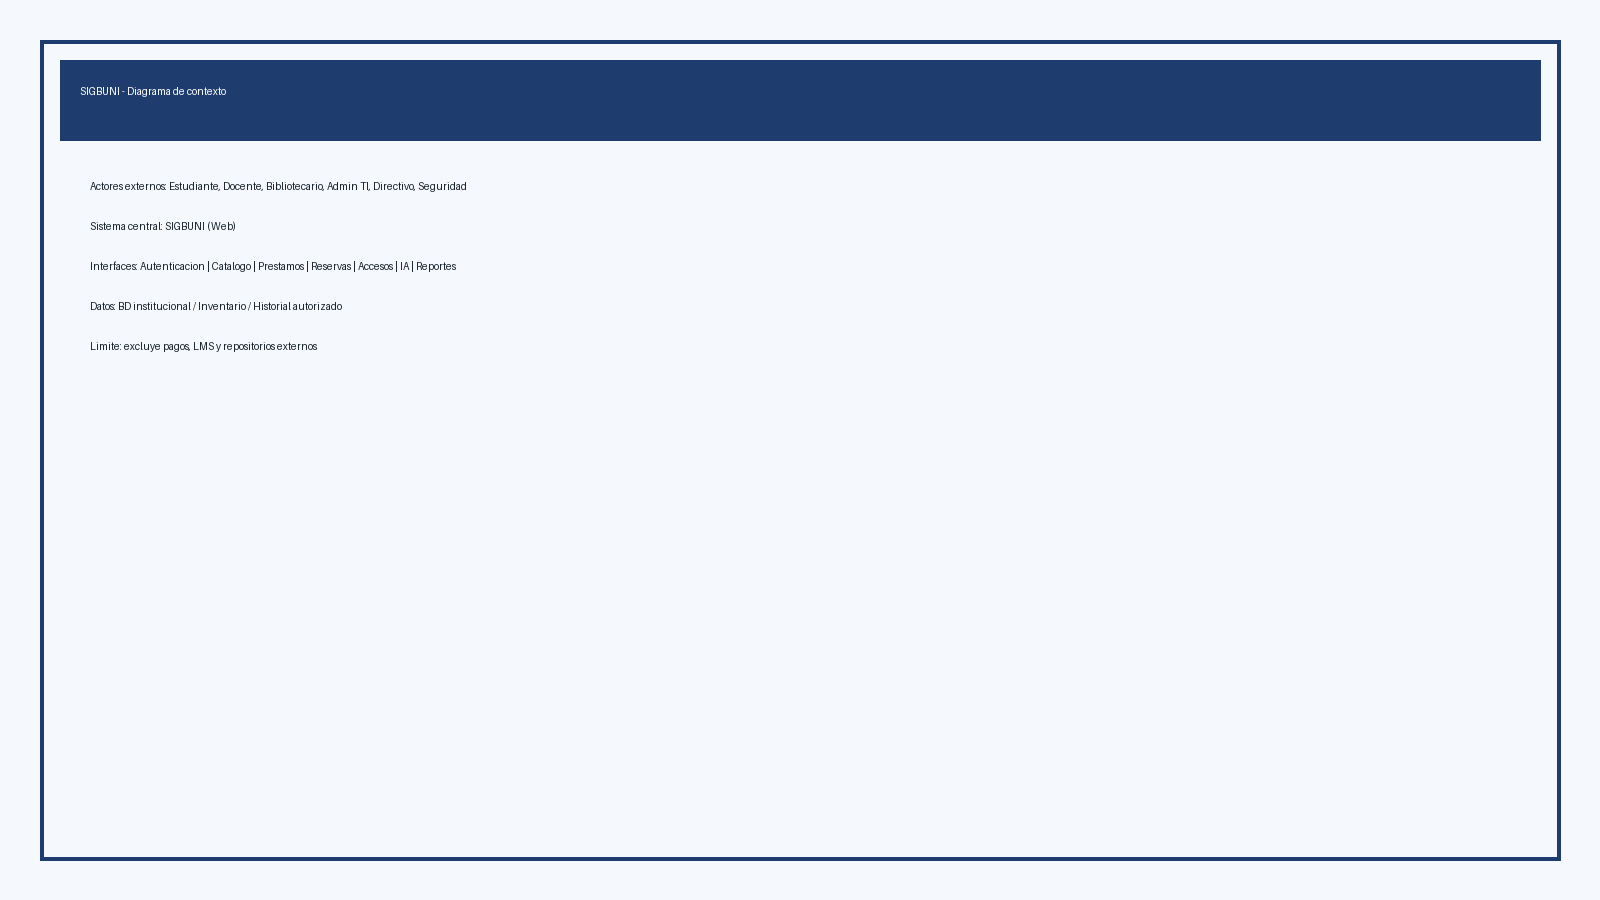
\includegraphics[width=0.96\textwidth]{diagrama_contexto.png}
\caption{Diagrama de contexto heredado de la Entrega 2 (1B).}
\label{fig:contexto}
\end{figure}

\subsection{Funciones del producto}
\begin{longtable}{P{0.12\textwidth}P{0.82\textwidth}}\toprule
\textbf{ID} & \textbf{Función de alto nivel}\\\midrule\endfirsthead
\toprule\textbf{ID} & \textbf{Función de alto nivel}\\\midrule\endhead
FP-01 & Gestionar préstamo, devolución y renovación de materiales.\\
FP-02 & Mantener un catálogo digital actualizado y consultable.\\
FP-03 & Permitir la reserva digital de espacios físicos.\\
FP-04 & Registrar ingreso y salida mediante control de acceso.\\
FP-05 & Gestionar usuarios, roles y permisos.\\
FP-06 & Enviar notificaciones internas.\\
FP-07 & Atender consultas frecuentes mediante chatbot.\\
FP-08 & Recomendar materiales según carrera, historial o tema.\\
FP-09 & Generar resúmenes automáticos cuando aplique.\\
FP-10 & Generar reportes estadísticos de uso, demanda y aforo.\\\bottomrule
\end{longtable}

\subsection{Clases y características de usuarios}
\begin{table}[H]\centering
\caption{Perfiles de usuario}
\begin{tabularx}{\textwidth}{P{0.20\textwidth}Y Y}\toprule
\textbf{Usuario} & \textbf{Características} & \textbf{Funciones principales}\\\midrule
Estudiante & Usuario frecuente que requiere acceso rápido al catálogo, préstamos, reservas, alertas y orientación. & Consultar catálogo, solicitar préstamos, reservar espacios, usar chatbot y recibir alertas.\\
Docente / investigador & Requiere materiales especializados, espacios y recomendaciones por área. & Buscar material, reservar salas, recibir recomendaciones y consultar disponibilidad.\\
Personal de biblioteca & Opera procesos diarios y mantiene la información actualizada. & Registrar préstamos, devoluciones, accesos, inventario y reportes.\\
Administrador TI & Configura seguridad, usuarios, permisos y soporte. & Gestionar roles, parámetros, respaldos e integraciones.\\
Directivo académico & Consulta información para toma de decisiones. & Visualizar reportes de demanda, aforo y uso.\\\bottomrule
\end{tabularx}
\end{table}

\subsection{Mapa de stakeholders}
\begin{table}[H]\centering
\caption{Matriz poder/interés}
\begin{tabularx}{\textwidth}{P{0.10\textwidth}P{0.28\textwidth}P{0.12\textwidth}P{0.12\textwidth}Y}\toprule
\textbf{ID} & \textbf{Stakeholder} & \textbf{Poder} & \textbf{Interés} & \textbf{Estrategia}\\\midrule
S-01 & Estudiantes & Alto & Alto & Gestionar de cerca y validar facilidad de uso.\\
S-02 & Docentes e investigadores & Alto & Medio & Consultar periódicamente.\\
S-03 & Personal de biblioteca & Alto & Alto & Gestionar de cerca por su criticidad operativa.\\
S-04 & Decanos y directivos & Medio & Bajo & Informar avances y entregar reportes ejecutivos.\\
S-05 & Área de TI & Alto & Medio & Mantener satisfecha y validar infraestructura y seguridad.\\
S-06 & Rectoría / Dirección académica & Alto & Bajo & Mantener informada como patrocinador institucional.\\\bottomrule
\end{tabularx}
\end{table}

\subsection{Entorno operativo}
El sistema operará como una aplicación web responsiva accesible desde navegadores modernos en computadoras, laptops, tabletas y teléfonos. El personal administrativo empleará estaciones de trabajo dentro de la biblioteca. El control de acceso podrá apoyarse en lector QR, cámara o credencial institucional, según la infraestructura disponible. Los datos se almacenarán en una base centralizada gestionada por TI.

\subsection{Suposiciones y dependencias}
\begin{longtable}{P{0.12\textwidth}P{0.28\textwidth}P{0.54\textwidth}}\toprule
\textbf{ID} & \textbf{Suposición/dependencia} & \textbf{Descripción}\\\midrule\endfirsthead
\toprule\textbf{ID} & \textbf{Suposición/dependencia} & \textbf{Descripción}\\\midrule\endhead
SD-01 & Conectividad institucional & Conexión estable a internet o red universitaria.\\
SD-02 & Datos actualizados & Catálogo e inventario mantenidos por personal autorizado.\\
SD-03 & Credenciales & Identificación universitaria válida.\\
SD-04 & Infraestructura TI & Servidor, base de datos, respaldo y mantenimiento.\\
SD-05 & Servicios de IA & Disponibilidad y configuración del módulo de IA.\\
SD-06 & Capacitación & Formación del personal para adoptar el flujo digital.\\\bottomrule
\end{longtable}

\subsection{Modelado organizacional i*}
Se modelan las dependencias intencionales entre estudiantes, personal de biblioteca, administración TI, directivos y el sistema SIGBUNI. El Diagrama de Dependencia Estratégica (SD) muestra \emph{quién depende de quién} para metas, tareas y recursos; el Diagrama de Razón Estratégica (SR) descompone el razonamiento interno de actores clave, incluyendo el módulo de IA y el cumplimiento de la LOPDP.
\begin{figure}[H]\centering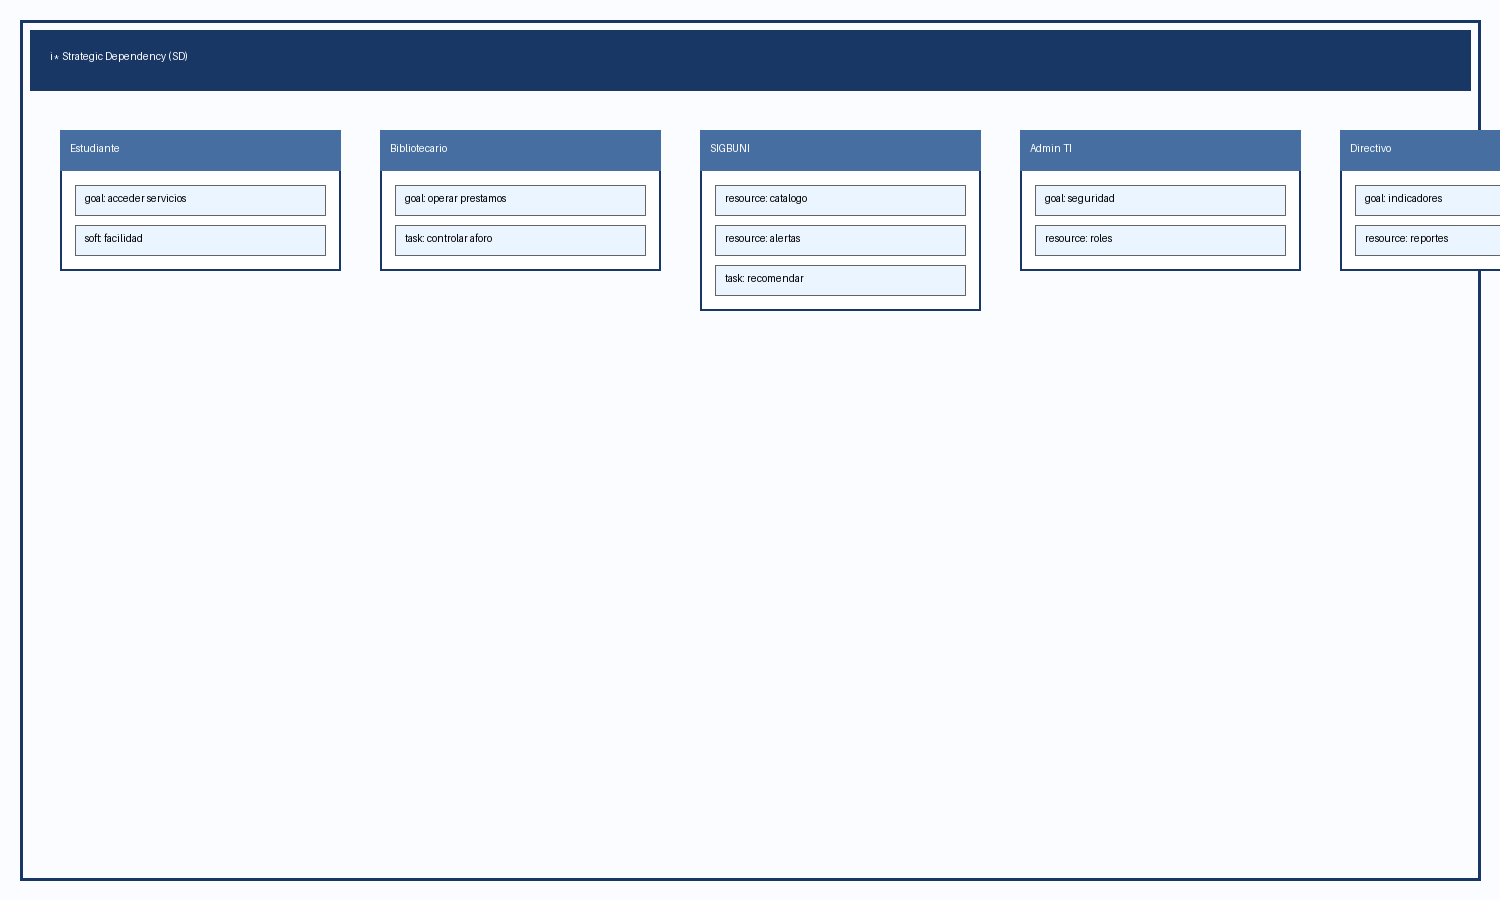
\includegraphics[width=0.92\textwidth]{ISTAR-SD.png}\caption{Diagrama i* de Dependencia Estratégica (SD).}\label{fig:istar-sd}\end{figure}
\begin{figure}[H]\centering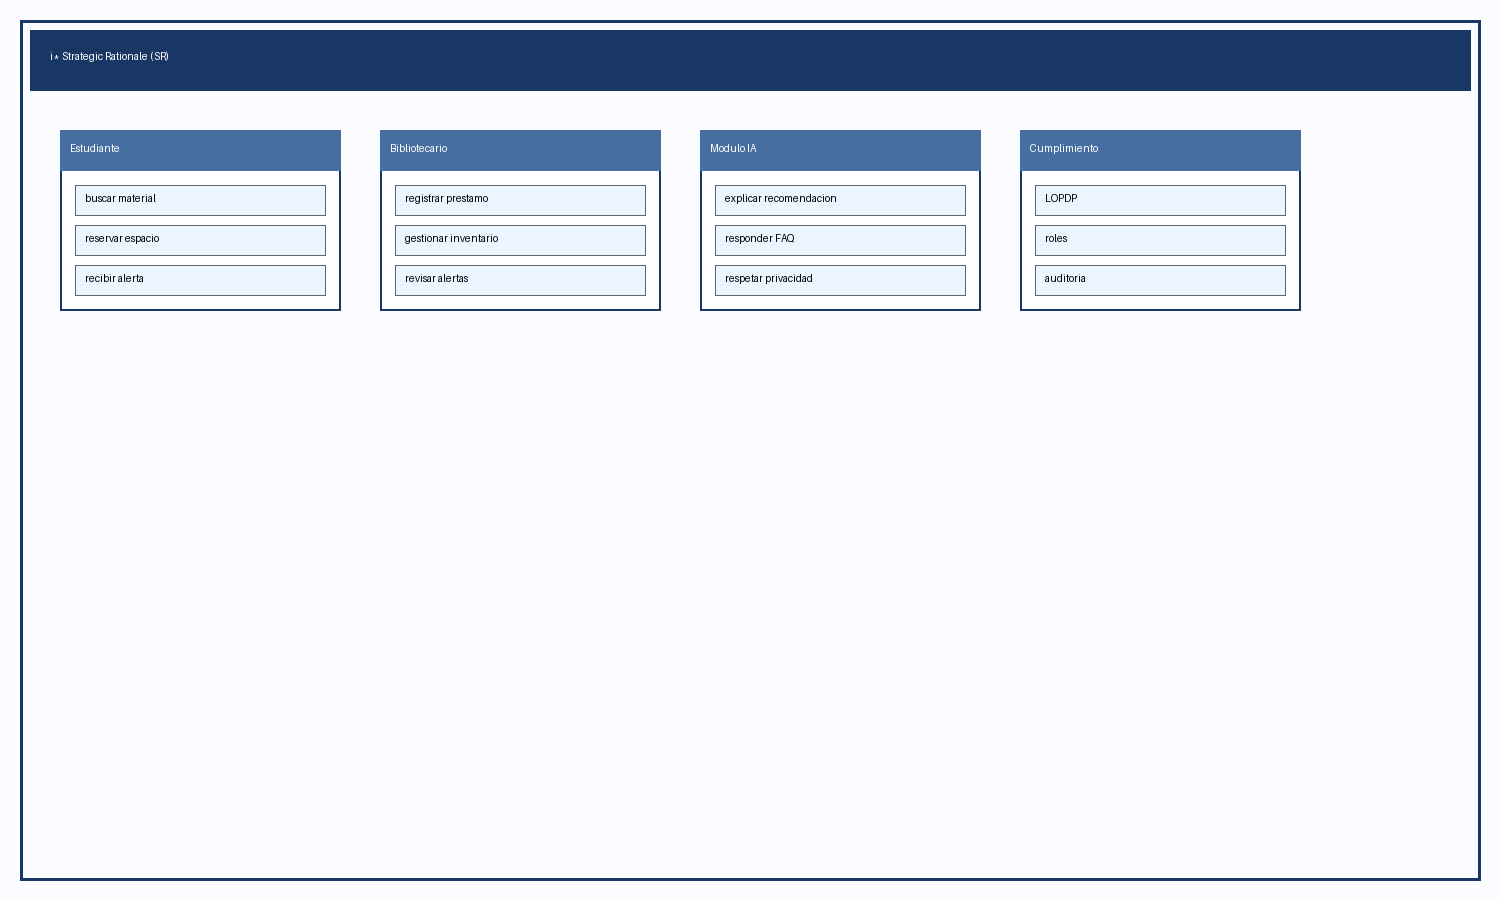
\includegraphics[width=0.92\textwidth]{ISTAR-SR.png}\caption{Diagrama i* de Razón Estratégica (SR).}\label{fig:istar-sr}\end{figure}

\section{Requisitos específicos completos}
\subsection{Interfaces externas}
\medskip\noindent\textbf{Interfaces de usuario}\par\smallskip
\begin{table}[H]\centering
\caption{Interfaces de usuario identificadas}
\begin{tabularx}{\textwidth}{P{0.12\textwidth}P{0.25\textwidth}Y}\toprule
\textbf{ID} & \textbf{Interfaz} & \textbf{Descripción}\\\midrule
IU-01 & Inicio de sesión & Autenticación con credenciales institucionales y validación de rol.\\
IU-02 & Catálogo digital & Búsqueda por título, autor, ISBN, área, carrera y estado.\\
IU-03 & Reserva de espacios & Selección de fecha, horario, espacio y confirmación.\\
IU-04 & Chatbot IA & Preguntas sobre servicios y orientación académica.\\
IU-05 & Panel bibliotecario & Gestión de préstamos, devoluciones, inventario, accesos y reportes.\\\bottomrule
\end{tabularx}
\end{table}

\begin{figure}[H]\centering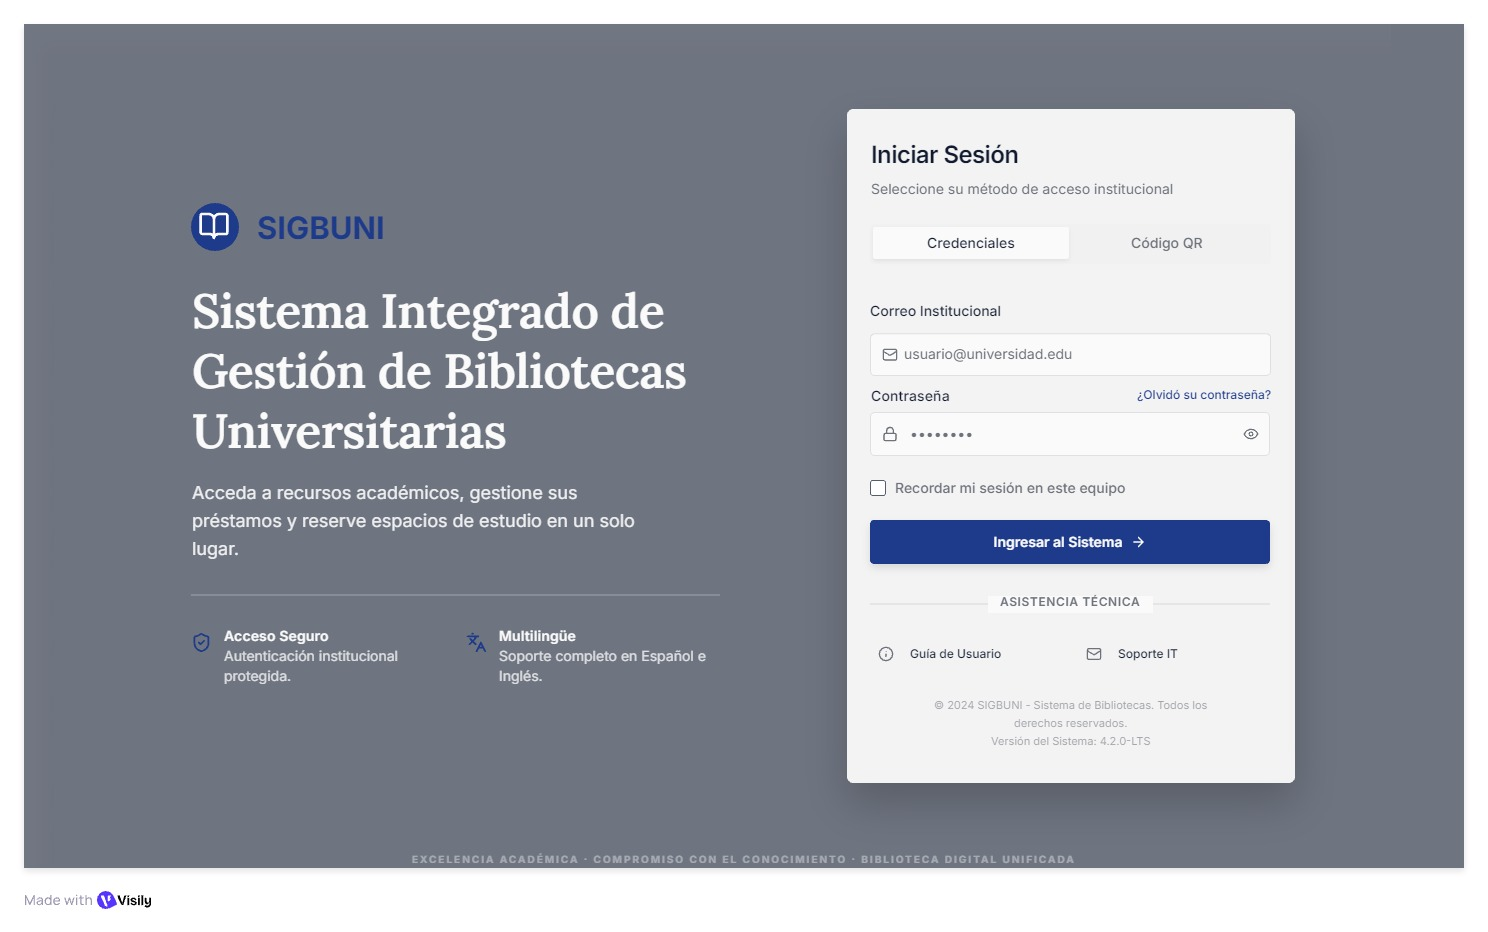
\includegraphics[width=0.82\textwidth]{MU-01_inicio_sesion.png}\caption{MU-01: mockup inicial de inicio de sesión.}\end{figure}
\begin{figure}[H]\centering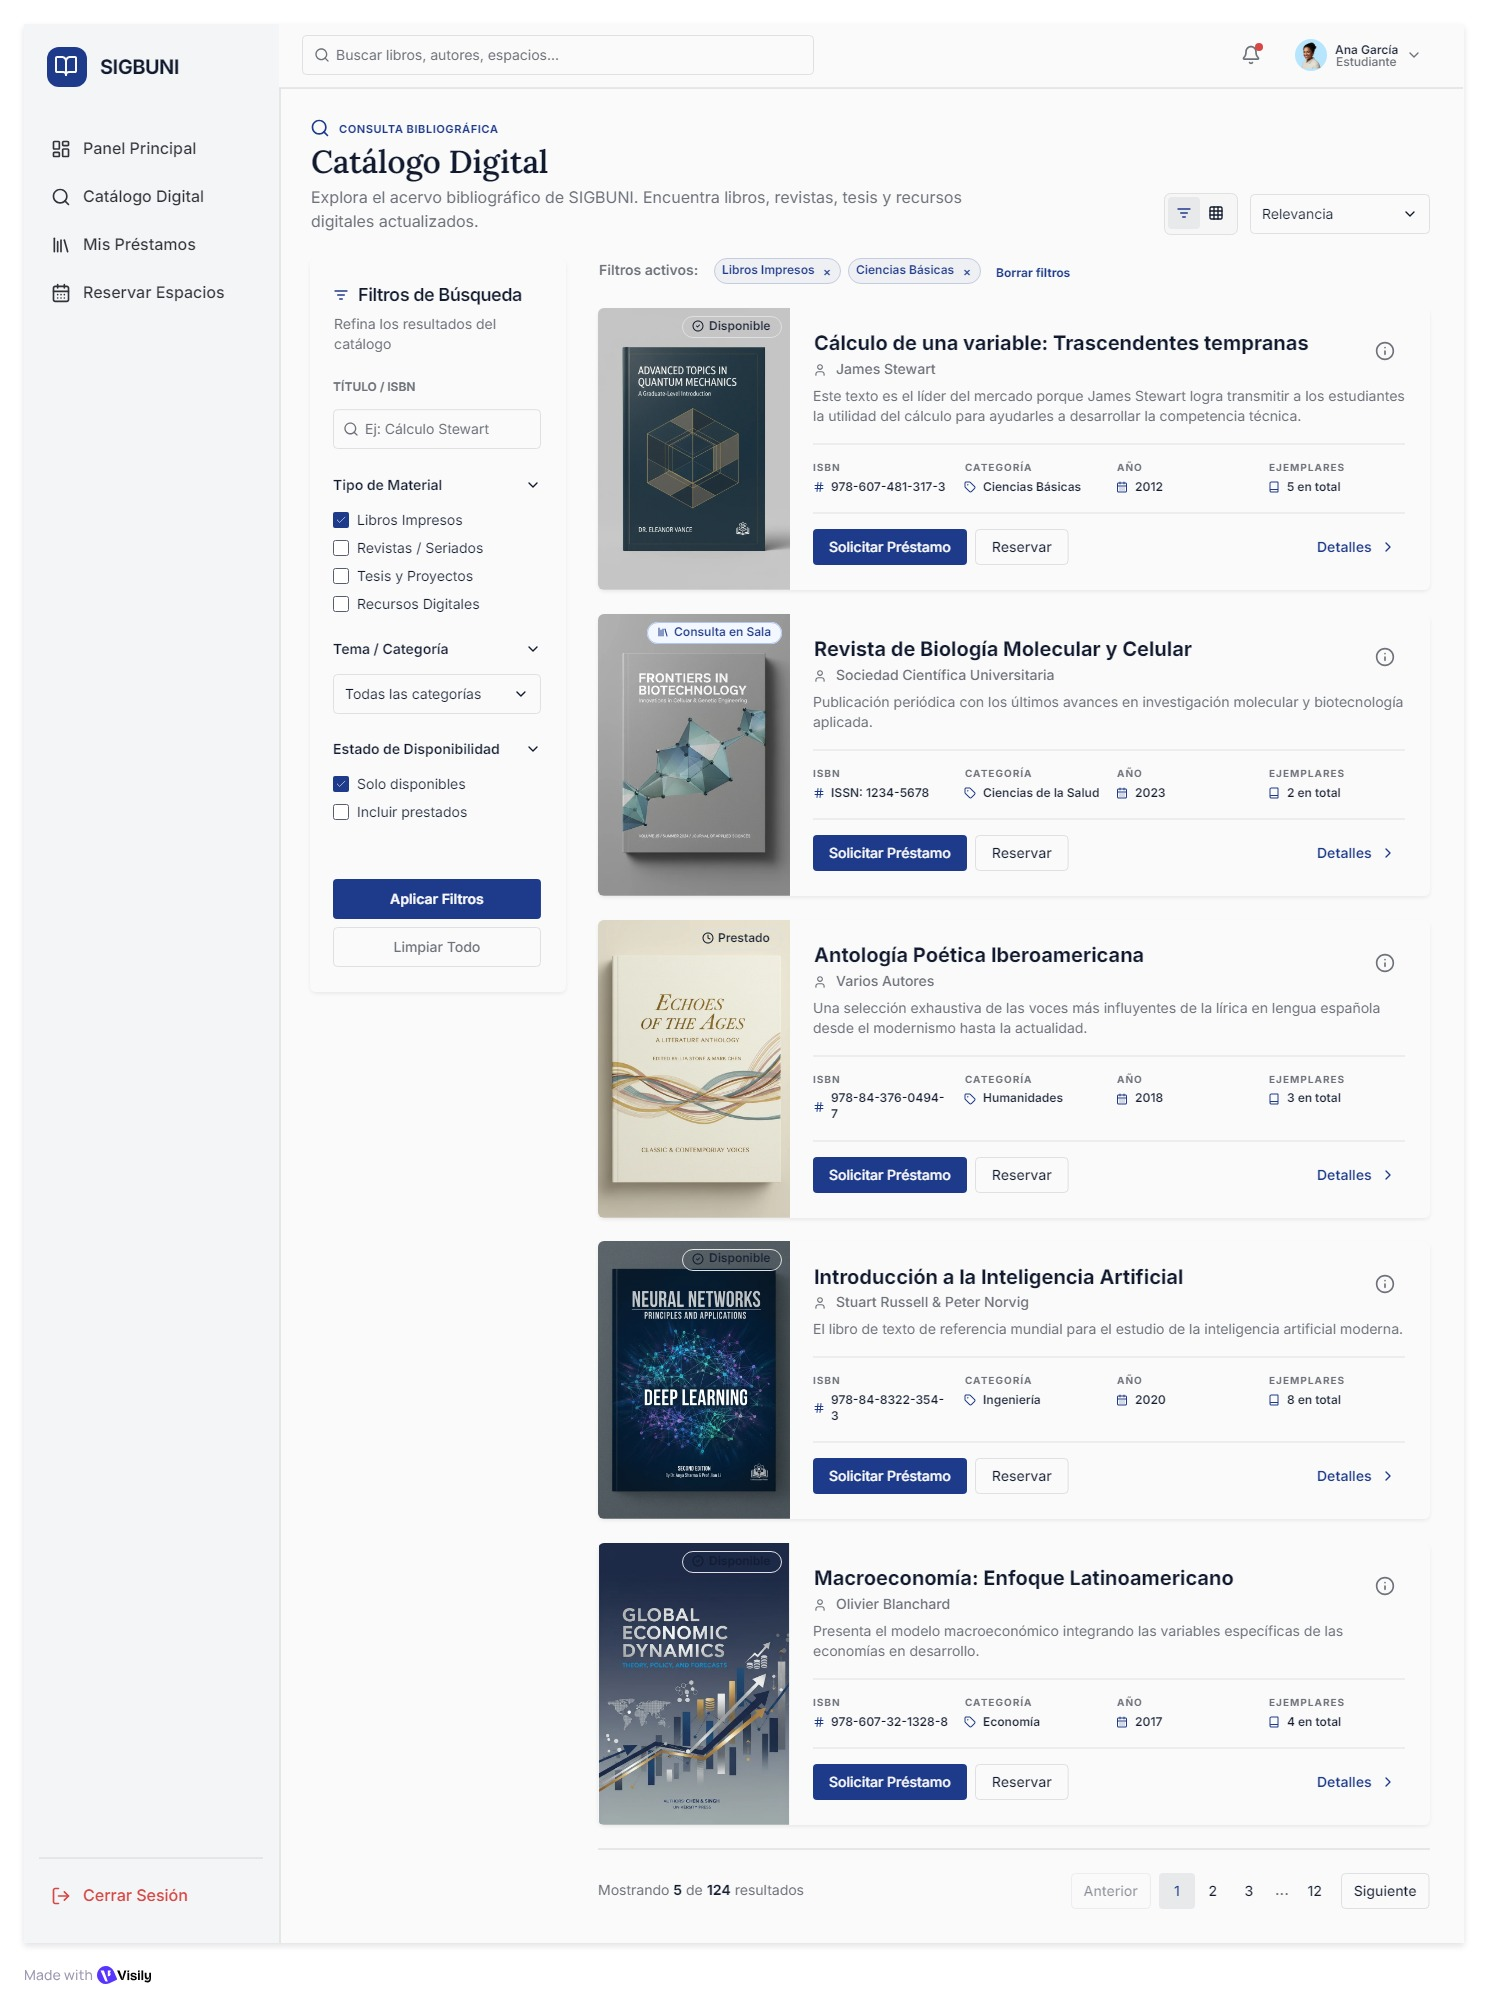
\includegraphics[width=0.82\textwidth]{MU-02_catalogo.png}\caption{MU-02: mockup inicial del catálogo digital.}\end{figure}
\begin{figure}[H]\centering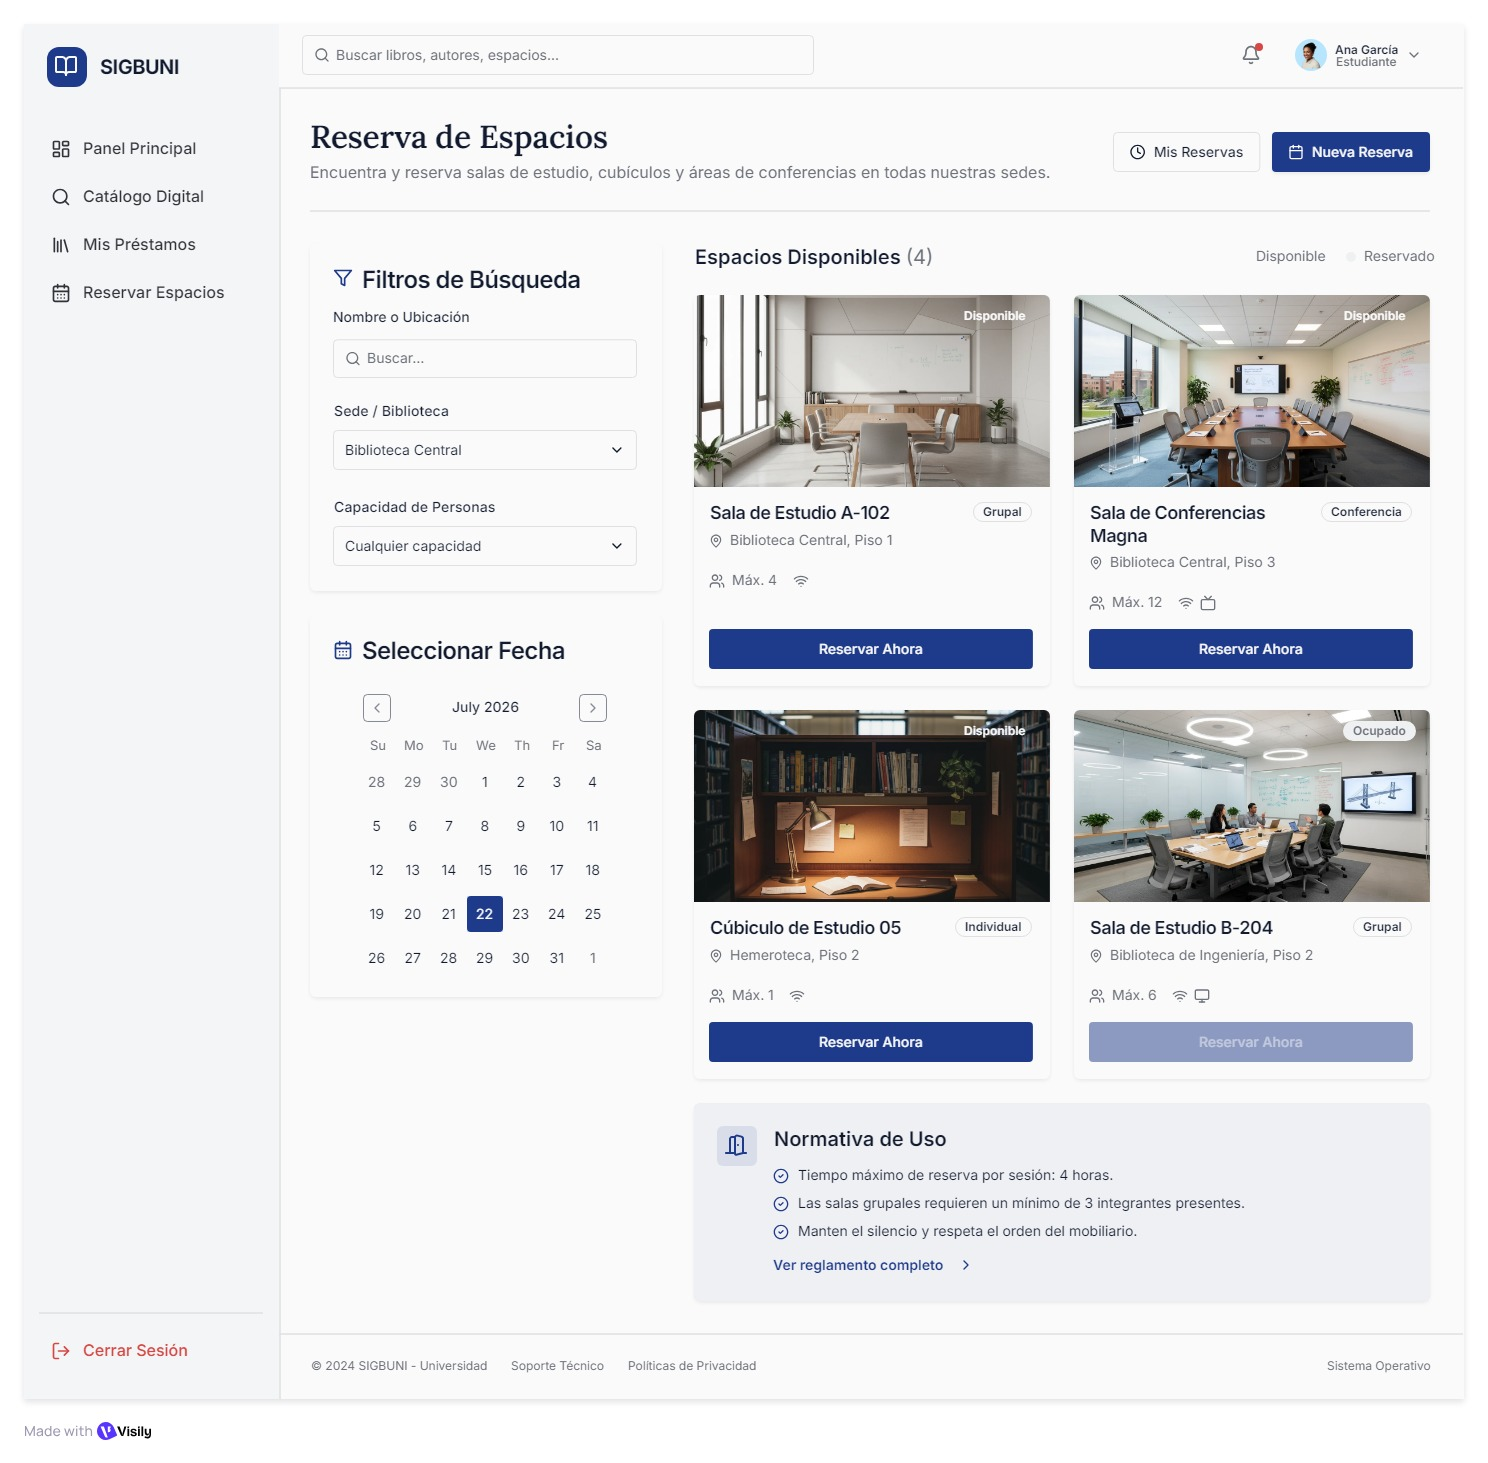
\includegraphics[width=0.82\textwidth]{MU-03_reserva_espacios.png}\caption{MU-03: mockup inicial de reserva de espacios.}\end{figure}
\begin{figure}[H]\centering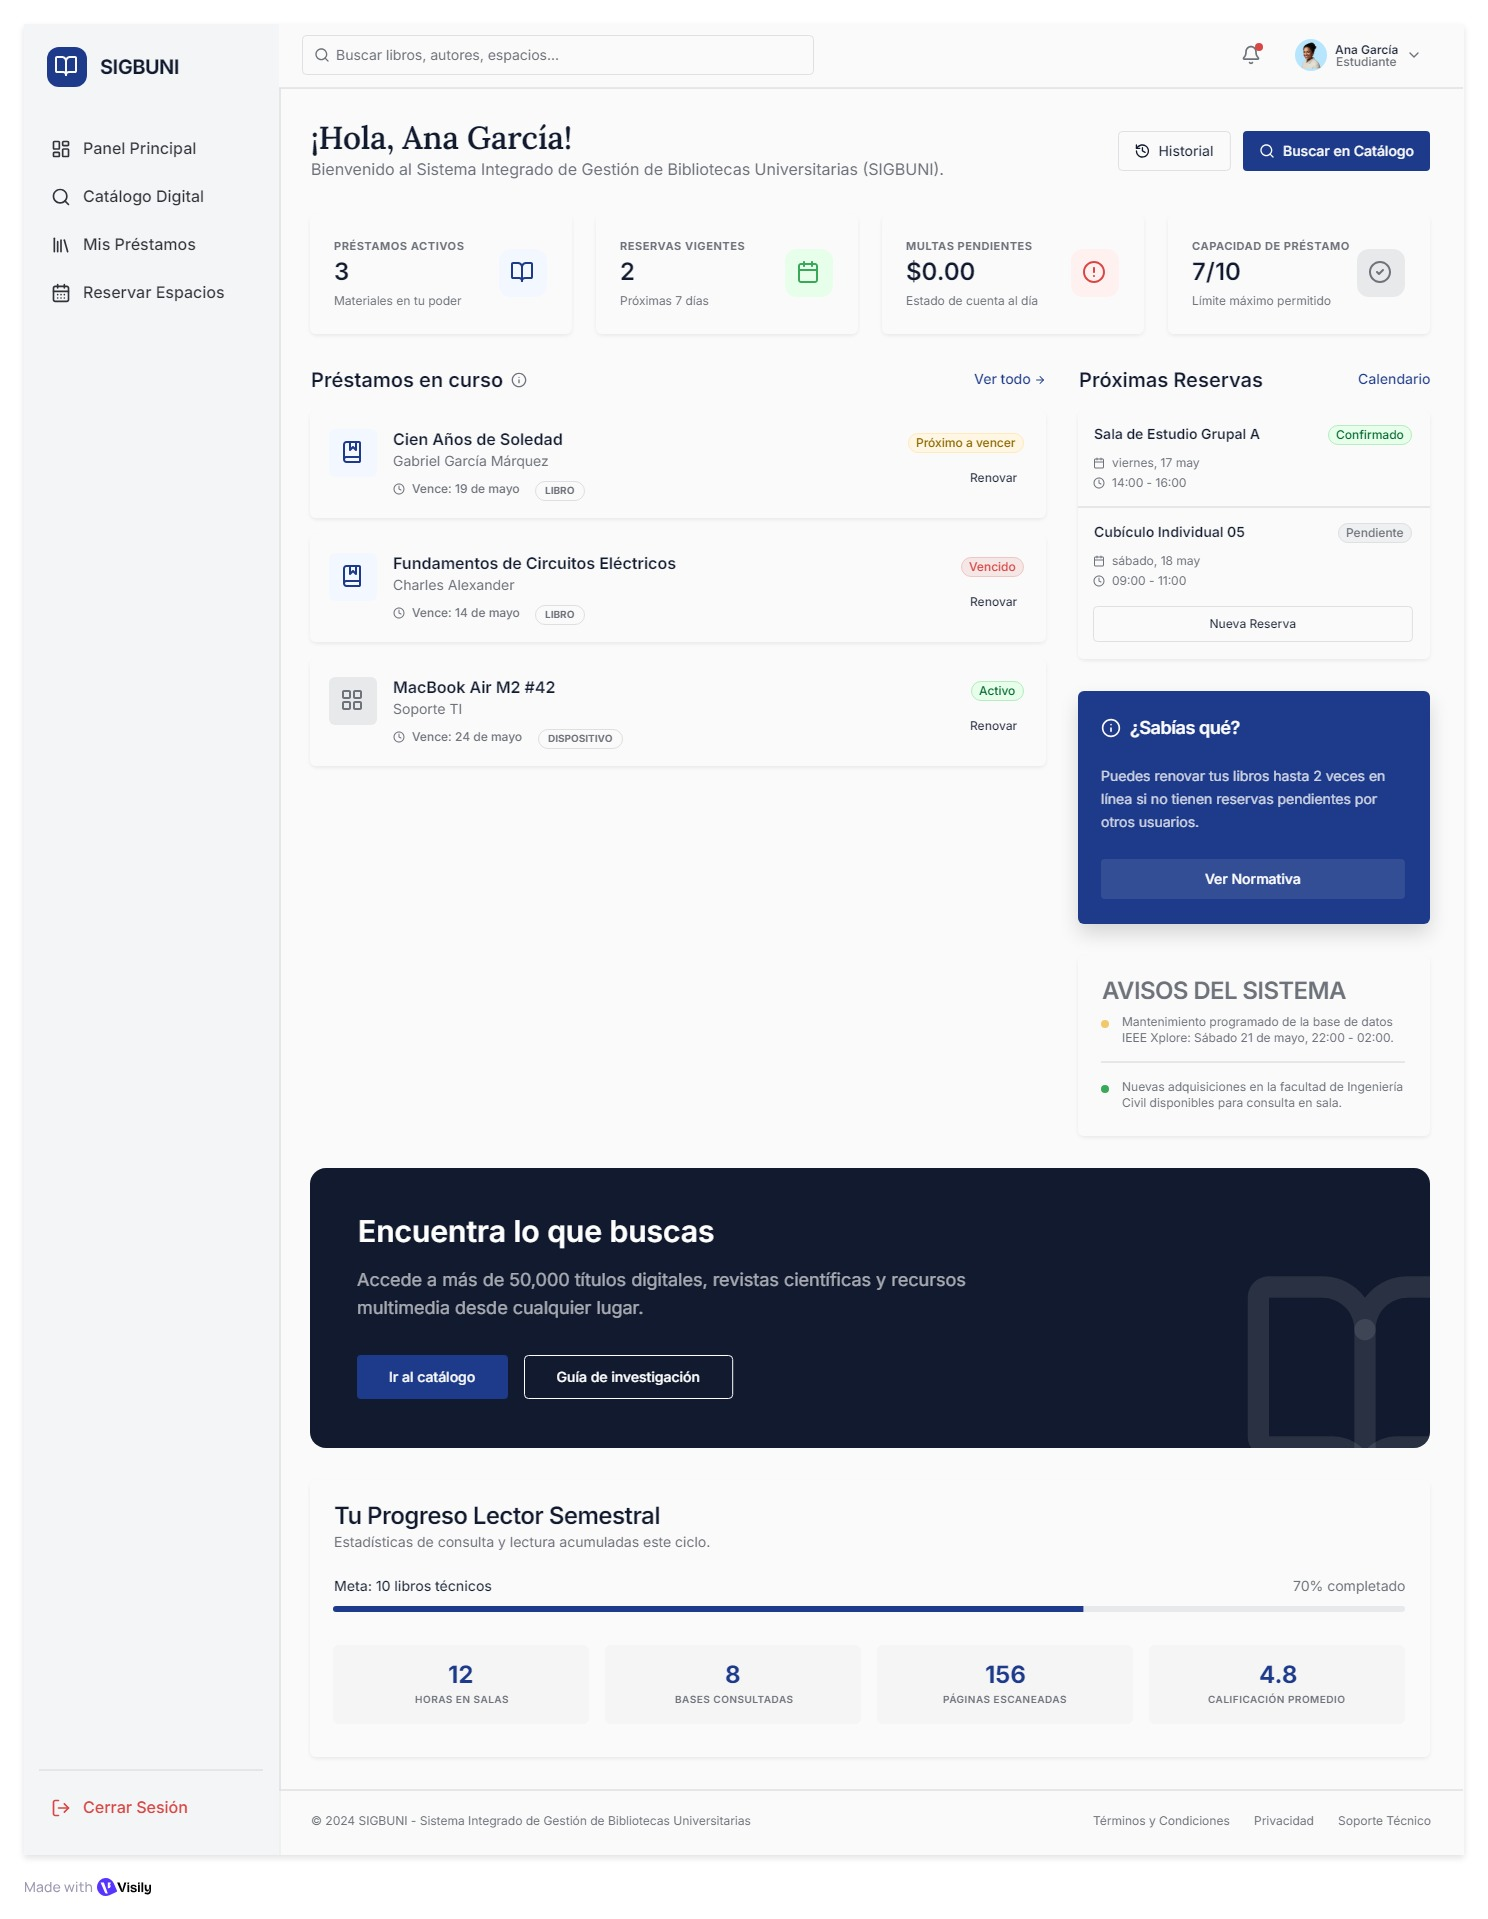
\includegraphics[width=0.82\textwidth]{MU-04_chatbot.png}\caption{MU-04: mockup inicial del chatbot.}\end{figure}
\begin{figure}[H]\centering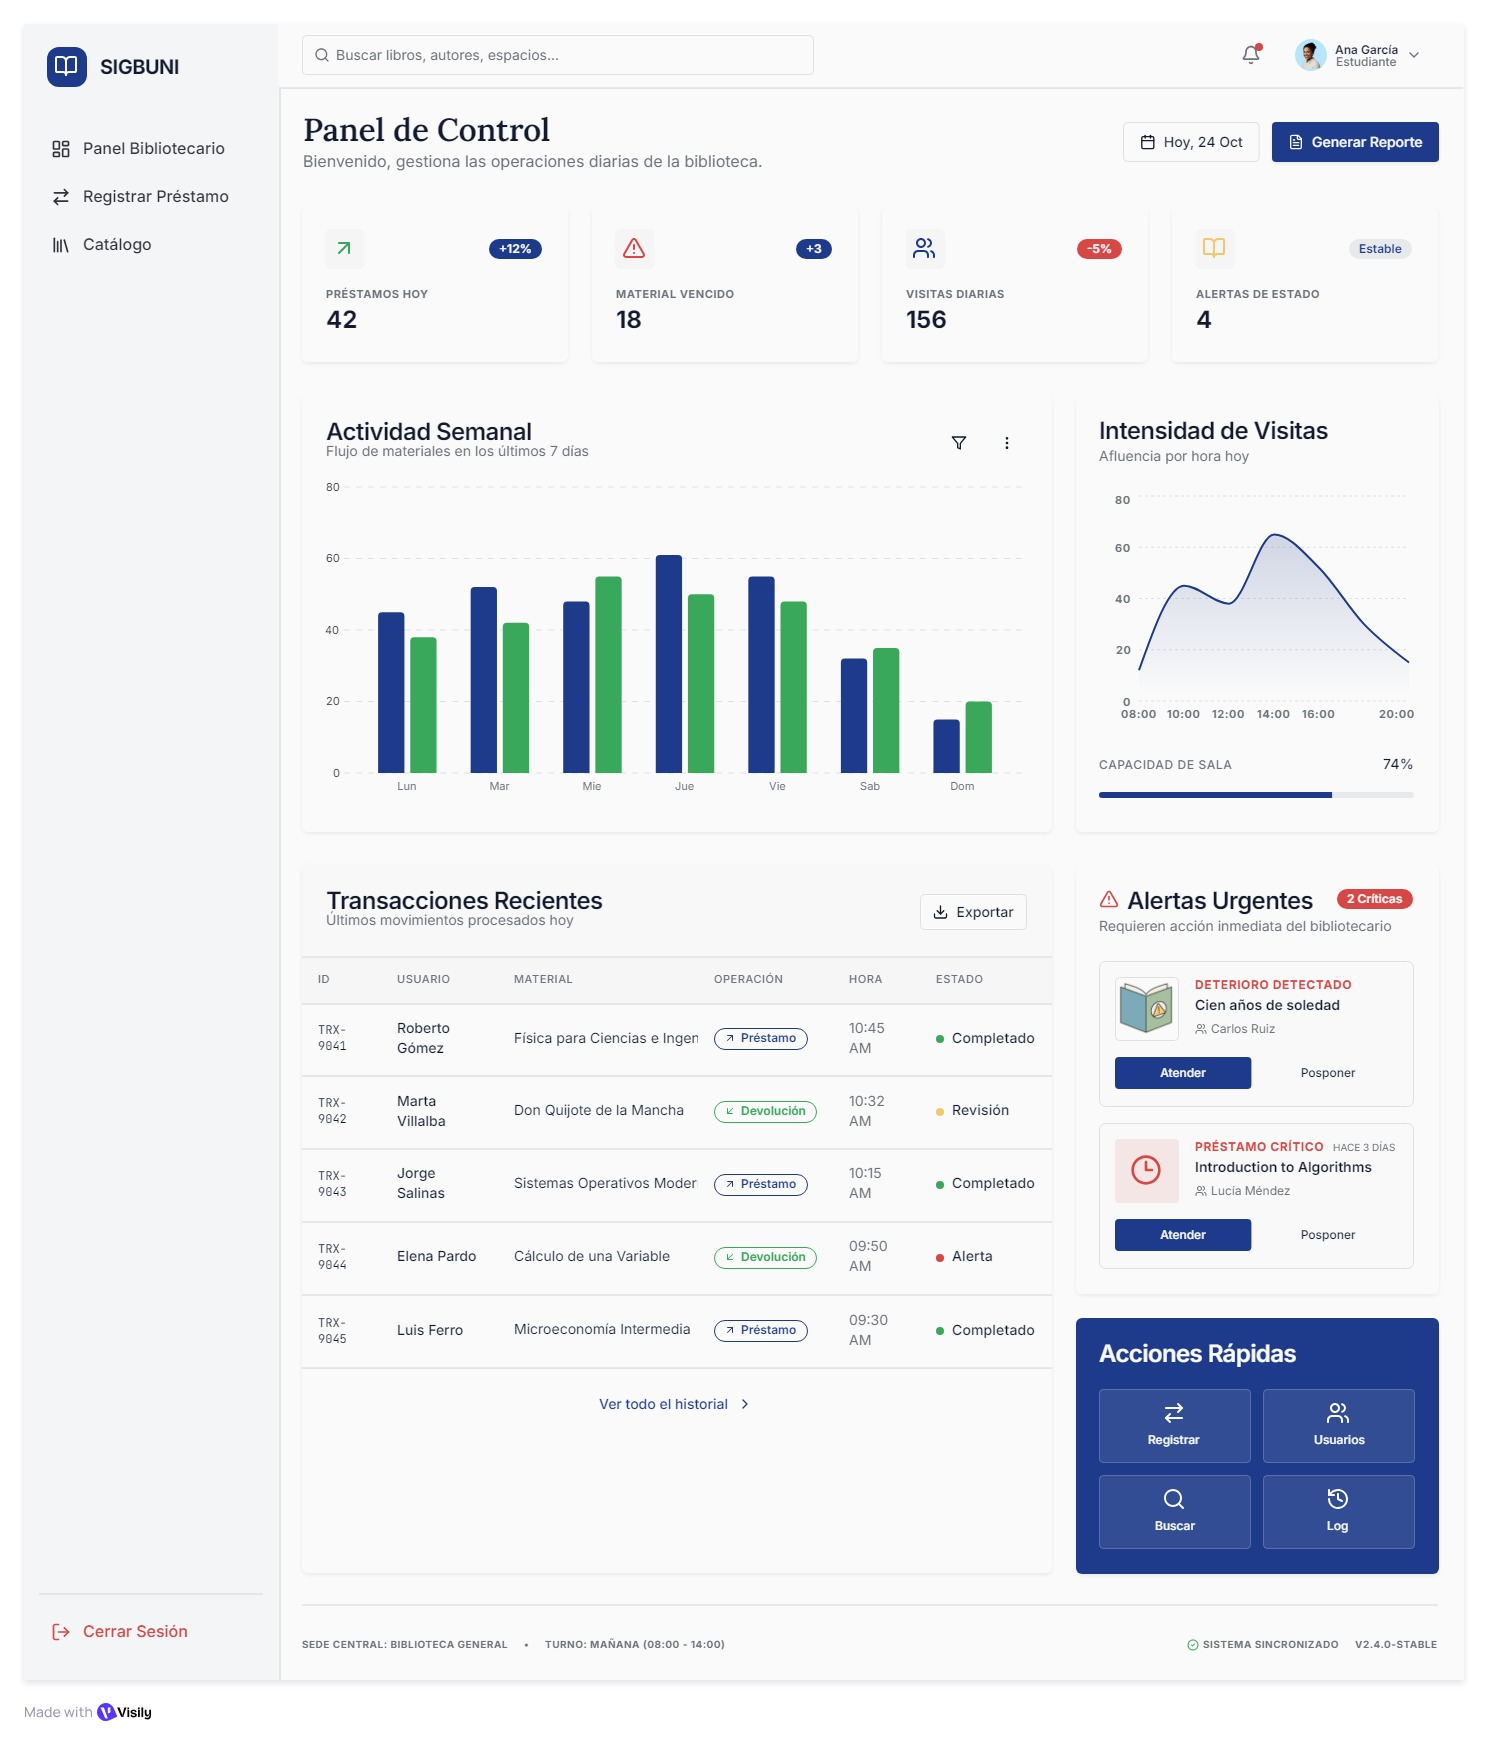
\includegraphics[width=0.82\textwidth]{MU-05_panel_bibliotecario.png}\caption{MU-05: mockup del panel bibliotecario.}\end{figure}
\begin{figure}[H]\centering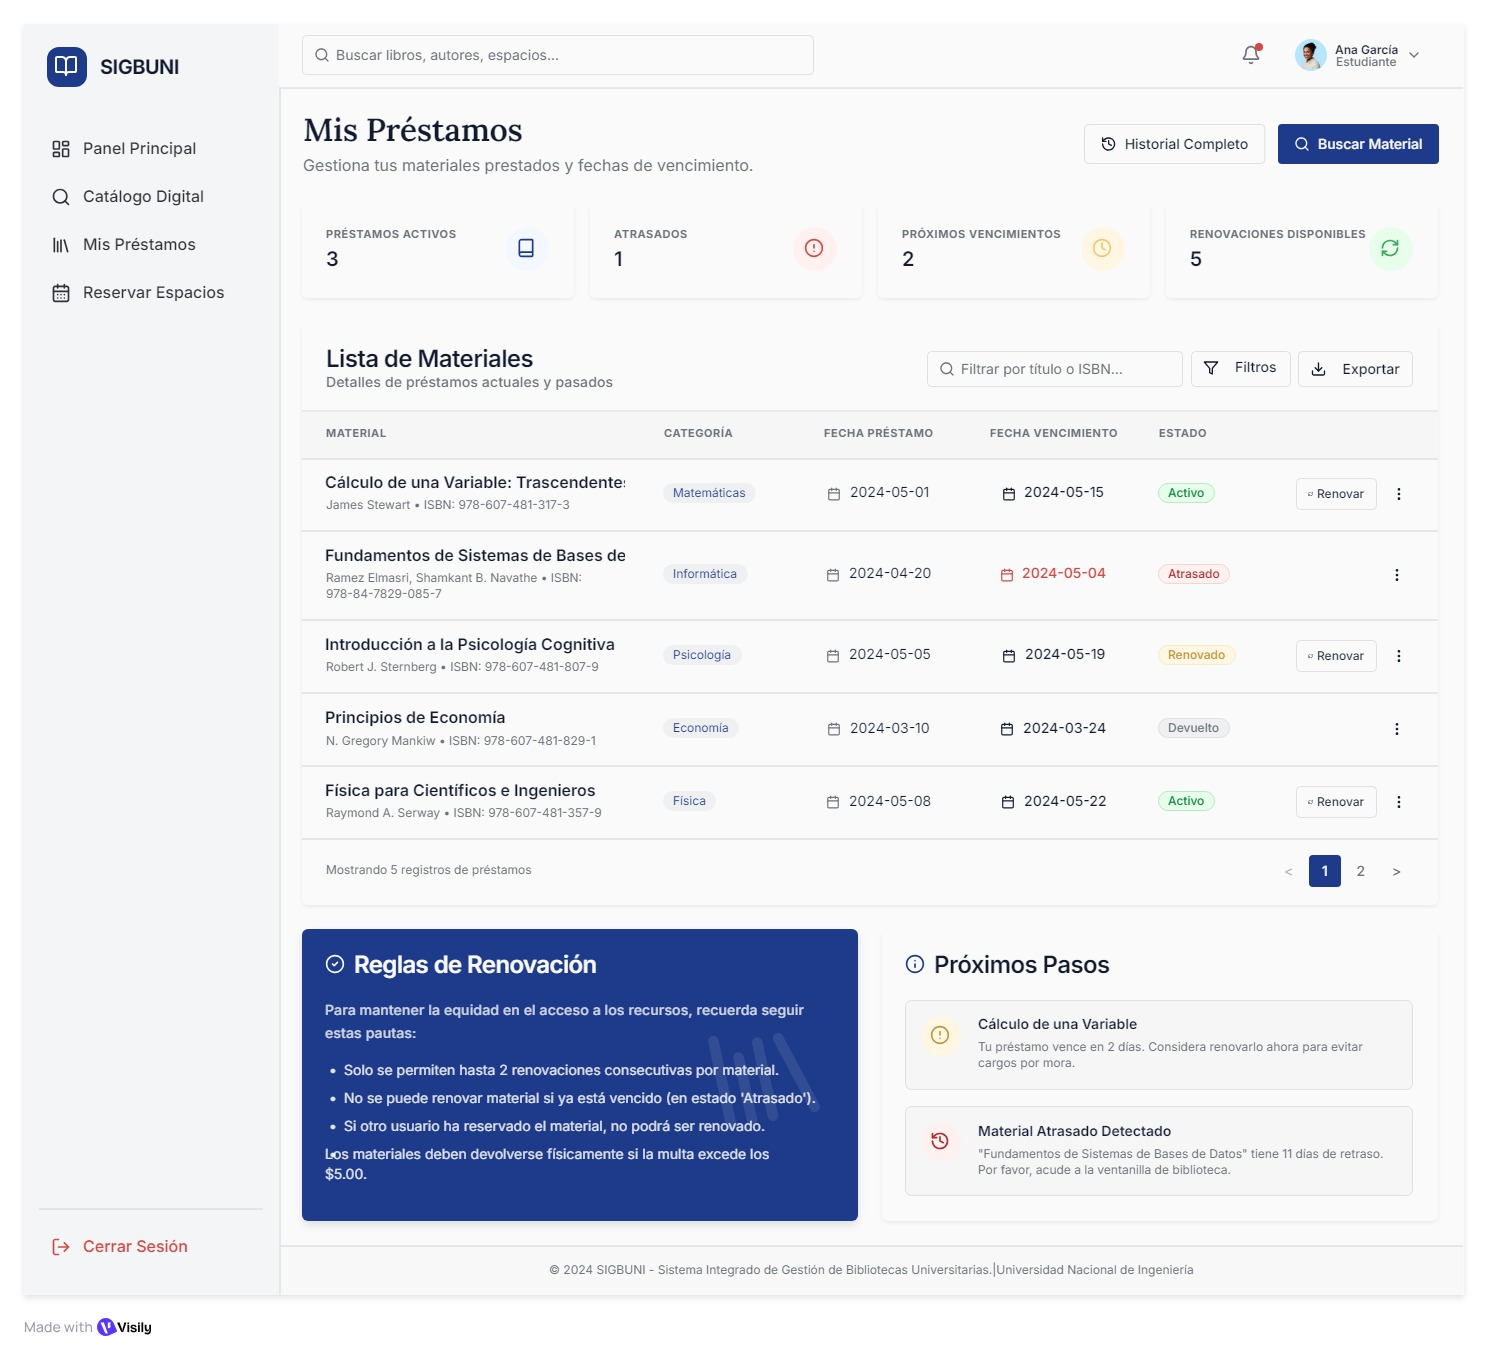
\includegraphics[width=0.82\textwidth]{MU-06_mis_prestamos.png}\caption{MU-06: mockup de mis préstamos.}\end{figure}
\begin{figure}[H]\centering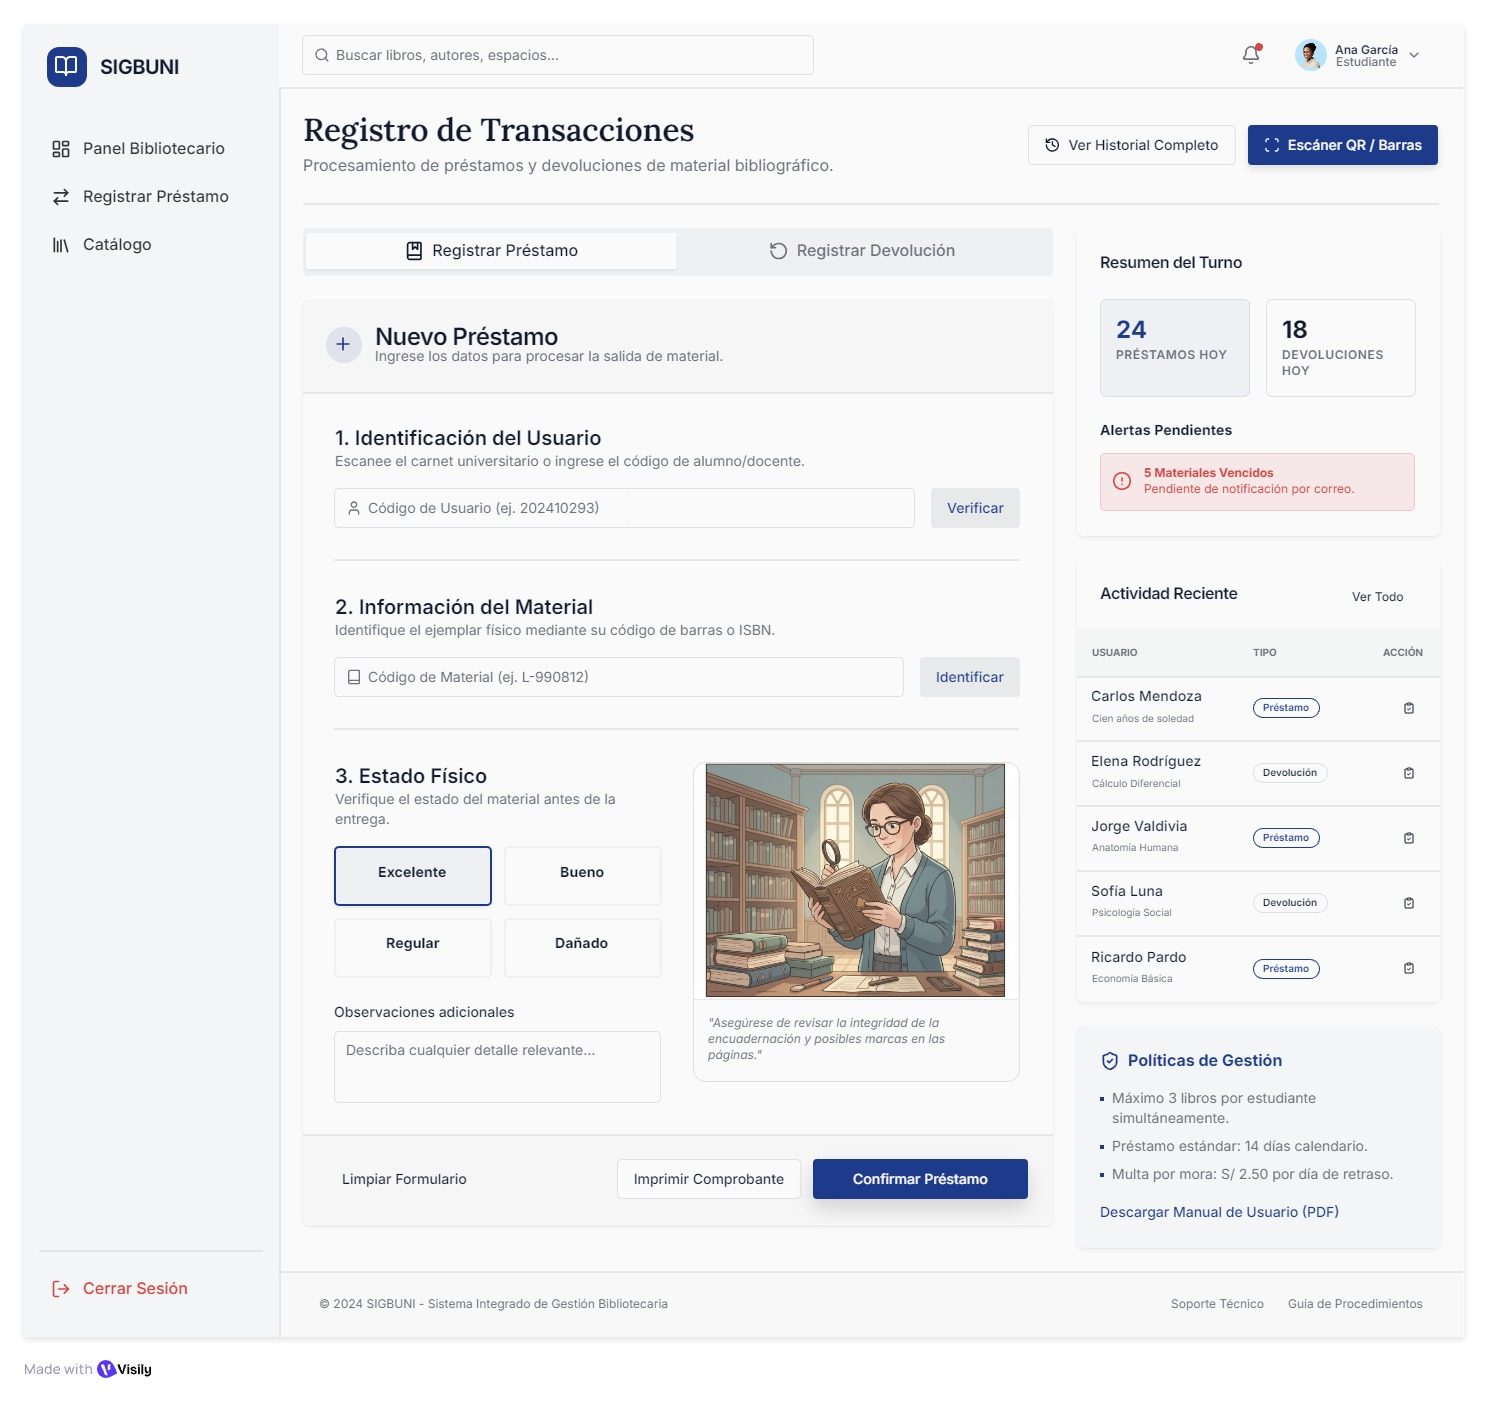
\includegraphics[width=0.82\textwidth]{MU-07_prestamo_devolucion.png}\caption{MU-07: mockup de préstamo y devolución.}\end{figure}
\begin{figure}[H]\centering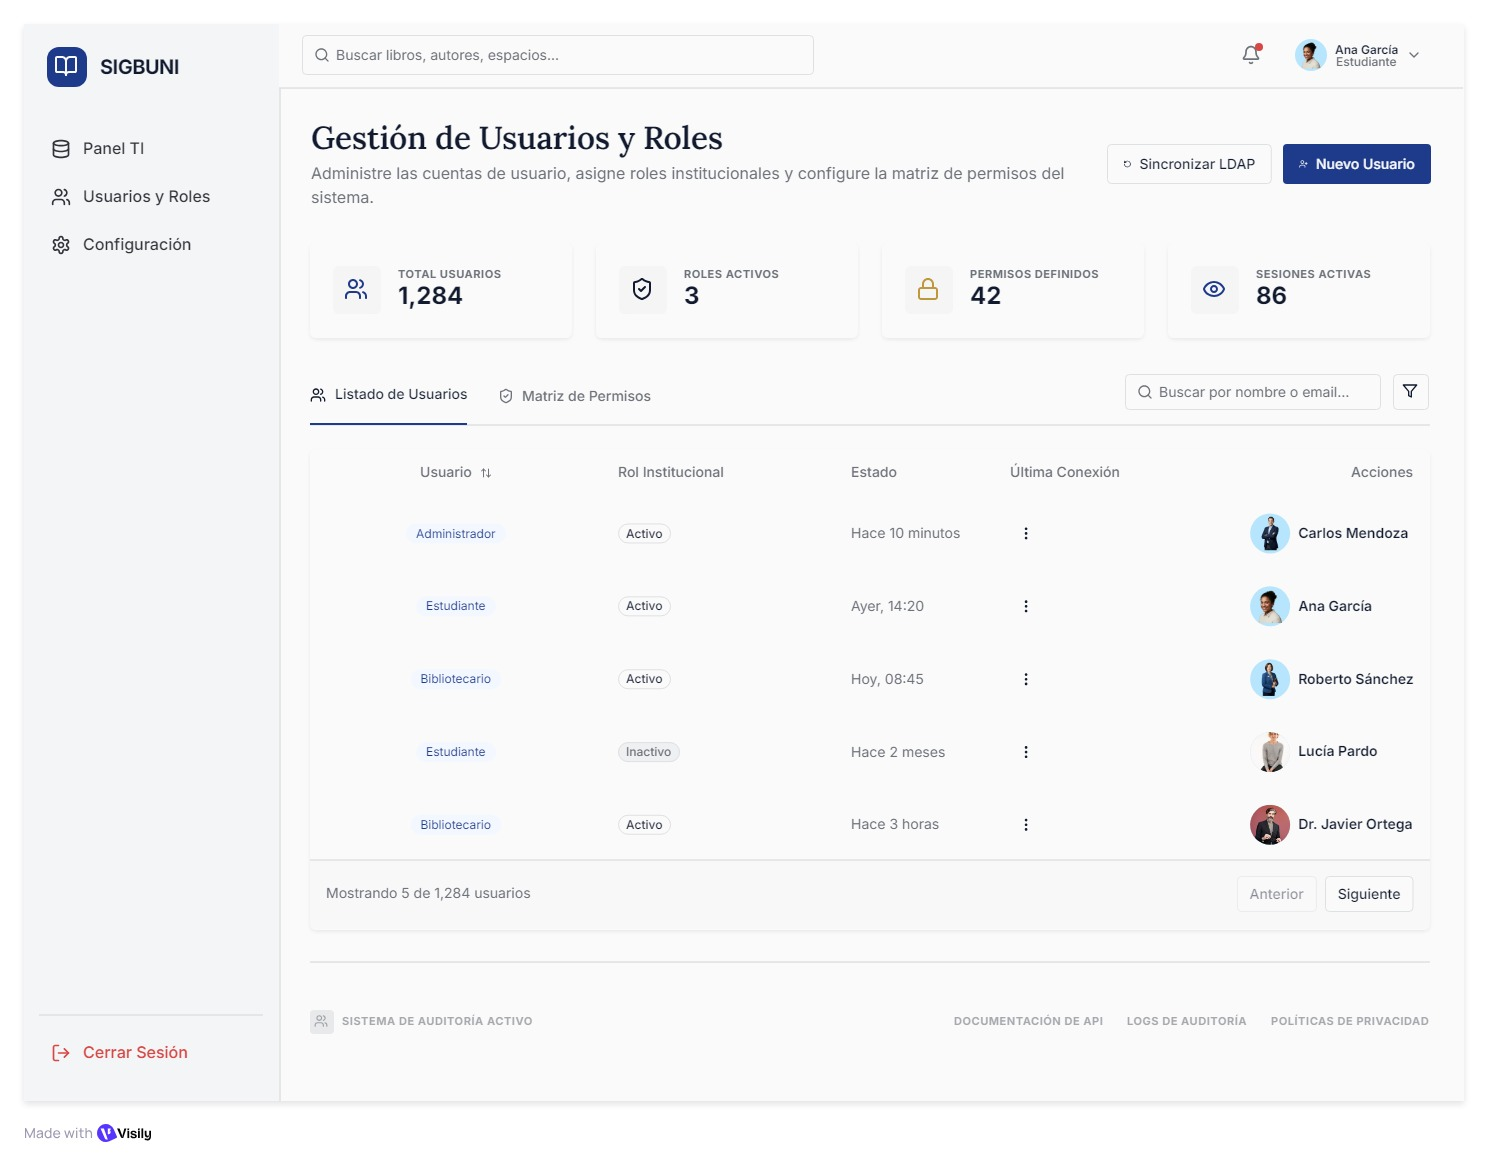
\includegraphics[width=0.82\textwidth]{MU-08_gestion_usuarios.png}\caption{MU-08: mockup de gestión de usuarios y roles.}\end{figure}
\begin{figure}[H]\centering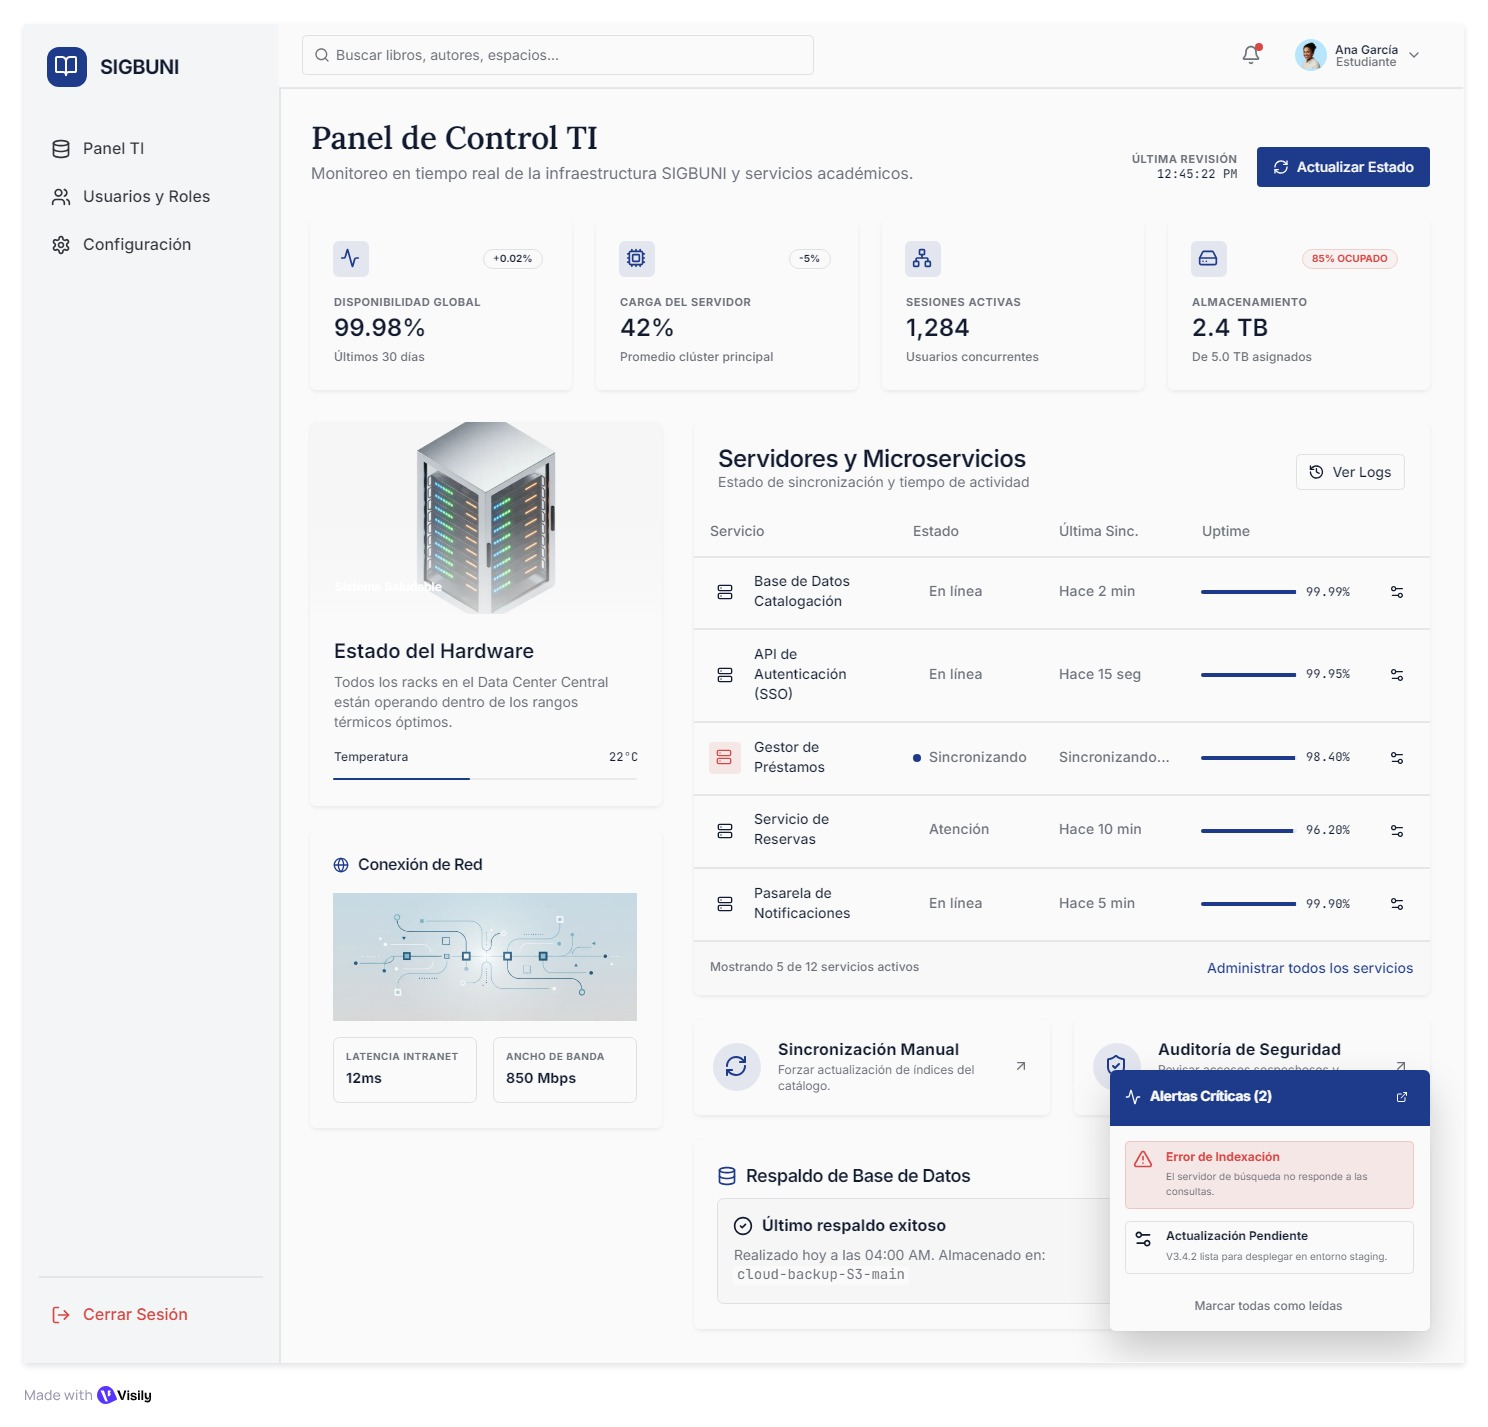
\includegraphics[width=0.82\textwidth]{MU-09_admin_ti.png}\caption{MU-09: mockup del panel administrador TI.}\end{figure}

\begin{table}[H]\centering
\caption{Trazabilidad inicial de mockups}
\begin{tabularx}{\textwidth}{P{0.13\textwidth}P{0.28\textwidth}Y P{0.16\textwidth}}\toprule
\textbf{Mockup} & \textbf{Pantalla} & \textbf{RF soportados} & \textbf{Estado}\\\midrule
MU-01 & Inicio de sesión & RF-17 y RNF de seguridad/autorización & Baseline; elevar a alta fidelidad.\\
MU-02 & Catálogo digital & RF-06, RF-07, RF-08 & Baseline; elevar a alta fidelidad.\\
MU-03 & Reserva de espacios & RF-09, RF-10, RF-11 & Baseline; elevar a alta fidelidad.\\
MU-04 & Chatbot IA & RF-04, RF-14, RF-15, RF-16, RF-20 & Baseline; elevar a alta fidelidad y agregar explicación.\\
MU-05 & Panel bibliotecario & RF-01, RF-02, RF-05, RF-17, RF-18, RF-19, RF-23, RF-25 & Alta fidelidad (Visily).\\
MU-06 & Mis préstamos & RF-21, RF-03, RF-04 & Alta fidelidad (Visily).\\
MU-07 & Préstamo y devolución & RF-01, RF-02 & Alta fidelidad (Visily).\\
MU-08 & Gestión de usuarios y roles & RF-17, RF-22 & Alta fidelidad (Visily).\\
MU-09 & Panel administrador TI & RF-17, RNF-03, RNF-08 & Alta fidelidad (Visily).\\\bottomrule
\end{tabularx}
\end{table}

\medskip\noindent\textbf{Interfaces de hardware}\par\smallskip
\begin{tabularx}{\textwidth}{P{0.30\textwidth}Y}\toprule
\textbf{Hardware} & \textbf{Uso}\\\midrule
Lector QR o cámara & Verificar credencial y registrar ingreso/salida.\\
Computadoras administrativas & Operar préstamos, devoluciones, inventario y reportes.\\
Servidor institucional & Alojar aplicación, base de datos y servicios.\\
Dispositivos móviles & Acceder a catálogo, reservas y chatbot.\\\bottomrule
\end{tabularx}

\medskip\noindent\textbf{Interfaces de software}\par\smallskip
\begin{tabularx}{\textwidth}{P{0.30\textwidth}Y}\toprule
\textbf{Software/servicio} & \textbf{Uso}\\\midrule
Base de datos centralizada & Almacenar usuarios, materiales, préstamos, reservas, accesos y notificaciones.\\
Módulo de IA & Procesar recomendaciones, consultas y resúmenes.\\
Servicio de autenticación & Validar credenciales y acceso por rol.\\
Notificaciones internas & Emitir alertas y comunicados.\\
GitHub & Versionar documentación, diagramas, evidencias y código.\\\bottomrule
\end{tabularx}

\subsection{Requisitos funcionales}
Los RF-01 a RF-20 se transcriben y reorganizan a partir de la Entrega 2 (1B). Los RF-21 a RF-25 se derivan de hallazgos ya documentados en EV-01--EV-15 y de pantallas Must presentes en los mockups Visily del repositorio (MU-01, MU-06, MU-07), sin introducir afirmaciones de campo no respaldadas.
\reqblock{RF-01}{Registrar préstamo bibliográfico}{El sistema debe permitir registrar el préstamo de un material bibliográfico a un usuario autorizado.}{Personal administrativo de biblioteca}{Código del usuario, código del material, fecha de préstamo y fecha esperada de devolución.}{Validar al usuario, verificar la disponibilidad, registrar el préstamo y cambiar el estado del material a prestado.}{Préstamo registrado y disponibilidad actualizada.}{Must}{EV-01, EV-15}
\reqblock{RF-02}{Registrar devolución de material}{El sistema debe permitir registrar la devolución de un material prestado.}{Personal administrativo de biblioteca}{Código del préstamo o material devuelto.}{Validar el préstamo activo, registrar la fecha real de devolución y actualizar el estado del material.}{Devolución registrada y material disponible o marcado según condición.}{Must}{EV-01}
\reqblock{RF-03}{Renovar préstamo digitalmente}{El sistema debe permitir renovar préstamos vigentes cuando no existan reservas pendientes del material.}{Estudiante / docente}{Solicitud de renovación y préstamo activo.}{Verificar vigencia, ausencia de reservas y límite de renovaciones; actualizar la fecha de devolución.}{Préstamo renovado o solicitud rechazada con motivo.}{Should}{EV-10}
\reqblock{RF-04}{Enviar notificación de vencimiento}{El sistema debe notificar al usuario cuando la fecha de devolución esté próxima a vencer.}{Sistema de notificaciones}{Préstamos próximos a vencer.}{Identificar préstamos con vencimiento cercano y generar una alerta interna al iniciar sesión.}{Notificación visible para el usuario.}{Must}{EV-01, EV-08}
\reqblock{RF-05}{Generar alerta por material vencido}{El sistema debe alertar al personal cuando un material no sea devuelto dentro del plazo establecido.}{Sistema / bibliotecario}{Fecha de devolución esperada vencida.}{Comparar la fecha actual con la fecha esperada y generar una alerta administrativa.}{Alerta de material vencido en el panel bibliotecario.}{Must}{EV-01}
\reqblock{RF-06}{Consultar catálogo digital}{El sistema debe permitir consultar el catálogo digital de materiales bibliográficos.}{Estudiante / docente / bibliotecario}{Criterio general de búsqueda.}{Recuperar materiales coincidentes desde la base de datos.}{Listado de materiales encontrados.}{Must}{EV-02, EV-13}
\reqblock{RF-07}{Buscar material por filtros}{El sistema debe permitir filtrar materiales por título, autor, ISBN, área temática, carrera o facultad afín.}{Usuario general}{Filtros seleccionados.}{Aplicar filtros y ordenar resultados según coincidencia.}{Resultados filtrados y legibles.}{Must}{EV-02}
\reqblock{RF-08}{Mostrar estado del material}{El sistema debe mostrar el estado actual de cada material: disponible, prestado, reservado, en mantenimiento o extraviado.}{Usuario general}{Selección o consulta de material.}{Consultar el inventario y presentar el estado actualizado.}{Estado visible del material.}{Must}{EV-02}
\reqblock{RF-09}{Reservar espacio bibliotecario}{El sistema debe permitir reservar cubículos, salas de estudio u otros espacios disponibles.}{Estudiante / docente}{Fecha, hora, espacio, usuario y motivo.}{Verificar disponibilidad y reglas de uso; registrar la reserva.}{Reserva confirmada o rechazada con motivo.}{Must}{EV-03, EV-15}
\reqblock{RF-10}{Mostrar disponibilidad de espacios}{El sistema debe mostrar en tiempo real los espacios disponibles para reserva.}{Usuario general}{Fecha y horario consultado.}{Consultar agenda de espacios y reservas vigentes.}{Calendario o listado de espacios disponibles.}{Must}{EV-03}
\reqblock{RF-11}{Liberar reserva por inasistencia}{El sistema debe liberar automáticamente una reserva si el usuario no se presenta en el tiempo límite configurado.}{Sistema}{Reserva confirmada y tiempo de tolerancia.}{Verificar la ausencia de confirmación de uso y cambiar el estado de la reserva.}{Espacio liberado y disponible para otros usuarios.}{Should}{EV-03}
\reqblock{RF-12}{Registrar ingreso a biblioteca}{El sistema debe registrar el ingreso del usuario al edificio mediante credencial, carnet o código QR.}{Personal de seguridad / sistema}{Identificación del usuario.}{Validar identidad y registrar fecha y hora de entrada.}{Ingreso registrado.}{Must}{EV-04}
\reqblock{RF-13}{Registrar salida de biblioteca}{El sistema debe registrar la salida del usuario para completar el control de permanencia.}{Personal de seguridad / sistema}{Identificación del usuario o registro abierto.}{Localizar el ingreso activo y registrar fecha y hora de salida.}{Salida registrada y permanencia calculada.}{Must}{EV-04}
\reqblock{RF-14}{Consultar chatbot de ayuda}{El sistema debe permitir realizar preguntas frecuentes sobre servicios de biblioteca mediante lenguaje natural.}{Estudiante / docente}{Pregunta del usuario.}{Procesar la consulta, identificar la intención y devolver una respuesta relacionada con servicios o procesos.}{Respuesta del chatbot mostrada en pantalla.}{Should}{EV-05}
\reqblock{RF-15}{Recomendar materiales con IA}{El sistema debe recomendar materiales bibliográficos según carrera, asignatura, tema o historial.}{Estudiante / docente}{Perfil académico, tema de consulta o historial autorizado.}{Analizar los datos disponibles y generar una lista de materiales sugeridos.}{Recomendaciones académicas ordenadas por relevancia.}{Should}{EV-05}
\reqblock{RF-16}{Generar resumen automático}{El sistema debe generar resúmenes automáticos de documentos extensos para orientar al usuario sobre su relevancia.}{Estudiante / docente}{Documento o texto autorizado para análisis.}{Procesar el contenido y producir una síntesis breve.}{Resumen automático visible para el usuario.}{Could}{EV-06}
\reqblock{RF-17}{Gestionar usuarios, roles y permisos}{El sistema debe permitir al administrador gestionar usuarios, roles y permisos de acceso.}{Administrador TI}{Datos de usuario, rol, estado y permisos.}{Crear, editar o desactivar usuarios y asignar roles según autorización.}{Usuarios y permisos actualizados.}{Must}{EV-09}
\reqblock{RF-18}{Generar reportes estadísticos}{El sistema debe generar reportes sobre préstamos, reservas, accesos, demanda y uso de servicios bibliotecarios.}{Directivo académico / bibliotecario}{Rango de fechas, tipo de reporte y filtros.}{Procesar registros históricos y consolidar indicadores.}{Reporte visual o exportable.}{Must}{EV-07, EV-14}
\reqblock{RF-19}{Enviar comunicados masivos}{El sistema debe permitir enviar comunicados a grupos de usuarios por rol, carrera o facultad.}{Administrador / bibliotecario}{Mensaje, destinatarios y fecha.}{Validar destinatarios, registrar el comunicado y publicarlo en el sistema.}{Comunicado visible para los usuarios seleccionados.}{Should}{EV-11}
\reqblock{RF-20}{Personalizar recomendaciones por historial}{El sistema debe mejorar las recomendaciones a partir de consultas y préstamos previos del usuario, respetando privacidad y permisos.}{Sistema de IA}{Historial autorizado del usuario.}{Analizar patrones de uso y actualizar sugerencias académicas.}{Recomendaciones personalizadas.}{Could}{EV-12}
\reqblock{RF-21}{Consultar mis préstamos}{El sistema debe permitir al usuario autenticado consultar sus préstamos activos, fechas de vencimiento y estado de renovación.}{Estudiante / docente}{Identidad del usuario autenticado.}{Recuperar préstamos asociados al usuario y presentarlos ordenados por fecha de vencimiento.}{Listado de préstamos propios con fechas y estado.}{Must}{EV-01, EV-08, EV-10}
\reqblock{RF-22}{Autenticar usuario institucional}{El sistema debe autenticar a los usuarios mediante credenciales institucionales y establecer la sesión según el rol autorizado.}{Usuario general / Administrador TI}{Credenciales institucionales.}{Validar credenciales, crear sesión y aplicar permisos del rol.}{Sesión iniciada o rechazo con mensaje de error sin exponer datos sensibles.}{Must}{EV-09}
\reqblock{RF-23}{Registrar y actualizar inventario}{El sistema debe permitir al personal de biblioteca registrar nuevos materiales y actualizar metadatos o estado del inventario.}{Personal administrativo de biblioteca}{Datos del material (título, autor, ISBN, área, estado).}{Validar campos obligatorios, persistir el material y reflejarlo en el catálogo.}{Material creado o actualizado en el inventario.}{Must}{EV-01, EV-02}
\reqblock{RF-24}{Cancelar reserva de espacio}{El sistema debe permitir cancelar una reserva vigente antes del inicio del horario reservado, liberando el espacio.}{Estudiante / docente}{Identificador de reserva y usuario propietario.}{Verificar titularidad y ventana de cancelación; cambiar estado a cancelada y liberar agenda.}{Reserva cancelada y espacio disponible.}{Should}{EV-03}
\reqblock{RF-25}{Consultar aforo en tiempo casi real}{El sistema debe mostrar al personal autorizado el aforo estimado a partir de ingresos y salidas registradas.}{Bibliotecario / directivo académico}{Registros de acceso del intervalo consultado.}{Calcular ocupantes activos y presentar indicador de aforo.}{Indicador de aforo visible en panel o reporte.}{Should}{EV-07, EV-14}

\subsection{Requisitos no funcionales}
Los RNF se cuantifican según ISO/IEC 25010:2023 \cite{iso25010_2023}. Se cubren las nueve características de calidad del producto y se añaden tres RNF de explicabilidad para los componentes de IA, tratados como NFR según \cite{chazette2020explainability,chazette2021exploring,chazette2022explainable}.

\begin{longtable}{P{0.10\textwidth}P{0.20\textwidth}P{0.48\textwidth}P{0.17\textwidth}}\toprule
\textbf{ID} & \textbf{Característica} & \textbf{Requisito cuantificado} & \textbf{Verificación / evidencia}\\\midrule\endfirsthead
\toprule\textbf{ID} & \textbf{Característica} & \textbf{Requisito cuantificado} & \textbf{Verificación / evidencia}\\\midrule\endhead
RNF-01 & Eficiencia de desempeño & El sistema deberá responder búsquedas del catálogo en máximo 2 segundos para el 95\% de las consultas en condiciones normales de red. & Prueba de rendimiento; EV-02.\\
RNF-02 & Fiabilidad / disponibilidad & Disponibilidad mínima del 99\% durante el horario académico definido (07:00--21:00). & Monitoreo mensual; EV-09.\\
RNF-03 & Seguridad & Bloqueo de sesión después de 15 minutos de inactividad. & Prueba funcional; EV-09.\\
RNF-04 & Interacción de usuario & Un usuario nuevo deberá completar una reserva en máximo 3 minutos con guía básica. & Prueba con usuarios; EV-03.\\
RNF-05 & Compatibilidad & Funcionamiento en versiones recientes de Chrome, Edge, Firefox y navegadores móviles Android/iOS de los últimos dos años. & Pruebas de compatibilidad; EV-13.\\
RNF-06 & Fiabilidad & No perder registros confirmados de préstamo, devolución o reserva ante fallos menores de conexión o recarga de página. & Prueba de persistencia; EV-01.\\
RNF-07 & Mantenibilidad & Organización modular (catálogo, préstamos, reservas, accesos, IA, usuarios y reportes) con acoplamiento bajo: un cambio de módulo no debe requerir modificar más de un módulo adicional. & Revisión de arquitectura; diagrama de componentes.\\
RNF-08 & Seguridad / privacidad & Datos personales, historial e ingresos visibles únicamente para roles autorizados; intentos no autorizados registrados. & Pruebas de autorización; EV-09; LOPDP.\\
RNF-09 & Adecuación funcional & El 100\% de los RF Must implementados en el MVP deben pasar sus escenarios Gherkin de aceptación en pruebas de integración. & Suite de aceptación; matriz HU/CA.\\
RNF-10 & Portabilidad & El despliegue local del MVP debe completarse en $\leq$ 30 minutos en un entorno Ubuntu LTS o Windows 11 con Docker Compose, sin cambios de código. & Prueba de instalación documentada en \path{05_MVP/README.md}.\\
RNF-11 & Flexibilidad & Parámetros de préstamo (días, renovaciones), tolerancia de reserva y umbral de aforo configurables por administrador sin redeploy de código. & Prueba de configuración; EV-03, EV-14.\\
RNF-12 & Explicabilidad de recomendaciones IA & Cada recomendación debe mostrar en $\leq$ 2\,s una explicación causal/por rasgos de $\leq$ 60 palabras (carrera, tema o historial autorizado); comprensión media $\geq$ 4/5 en Likert tras validación. & Walkthrough; EV-05; \cite{chazette2022explainable}.\\
RNF-13 & Explicabilidad de resúmenes IA & Todo resumen automático debe indicar fuente, longitud máxima (150 palabras) y advertencia de posible omisión; el usuario puede abrir el documento original en un clic. & Prueba funcional; EV-06.\\
RNF-14 & Explicabilidad del chatbot IA & Toda respuesta del chatbot debe etiquetarse como ``generada por IA'', incluir justificación breve o intención detectada y ofrecer derivación a atención humana cuando la confianza sea baja. & Prueba funcional + walkthrough; EV-05.\\
RNF-15 & Seguridad (refuerzo) & Contraseñas almacenadas con hash + salt; tráfico HTTPS; auditoría de cambios de roles retenida $\geq$ 12 meses. & Revisión de seguridad; EV-09; LOPDP Art.~26.\\\bottomrule
\end{longtable}

\subsection{Requisitos legales y trazabilidad con la LOPDP}
Se mapea la Ley Orgánica de Protección de Datos Personales del Ecuador \cite{lopdp2021} a requisitos de SIGBUNI. El mapeo es normativo-documental; la validación institucional del oficial de protección de datos permanece como actividad de seguimiento.

\begin{longtable}{P{0.14\textwidth}P{0.12\textwidth}P{0.30\textwidth}P{0.18\textwidth}P{0.18\textwidth}}\toprule
\textbf{Ley} & \textbf{Artículo} & \textbf{Obligación aplicable} & \textbf{RF/RNF} & \textbf{Evidencia}\\\midrule\endfirsthead
\toprule\textbf{Ley} & \textbf{Artículo} & \textbf{Obligación aplicable} & \textbf{RF/RNF} & \textbf{Evidencia}\\\midrule\endhead
LOPDP & Art.~4 y 7 & Licitud y consentimiento/base legítima para tratamiento de identificación y autenticación institucional. & RF-22, RNF-08 & EV-09; consentimientos.\\
LOPDP & Art.~12 & Registro de accesos y permanencia con finalidad de aforo y seguridad, minimizando datos. & RF-12, RF-13, RF-25 & EV-04, EV-14.\\
LOPDP & Art.~8 & Uso del historial para recomendaciones solo con base legítima/consentimiento y finalidad académica. & RF-15, RF-20, RNF-12 & EV-05, EV-12.\\
LOPDP & Art.~7 y 37 & Consentimiento informado y autorización para uso de datos anonimizados en publicaciones científicas. & Protocolo ético; dataset FAIR & Consentimientos firmados.\\
LOPDP & Art.~13--15 & Derechos de acceso, rectificación, eliminación y oposición sobre datos personales del usuario. & RF-17, RF-21, RNF-08 & EV-09.\\
LOPDP & Art.~26--27 & Seguridad, conservación, confidencialidad y respuesta ante incidentes de seguridad. & RNF-03, RNF-08, RNF-15, RD-04 & EV-09.\\\bottomrule
\end{longtable}

\subsection{Historias de usuario y criterios de aceptación para RF Must}
Cada RF Must se expresa en formato Connextra, se verifica INVEST y se acompaña de un escenario Gherkin derivado de la especificación del RF y de la evidencia asociada. La aceptación formal con stakeholders se confirma en las sesiones walkthrough (Sección de validación).

\begin{longtable}{P{0.09\textwidth}P{0.30\textwidth}P{0.18\textwidth}P{0.35\textwidth}}\toprule
\textbf{RF} & \textbf{Historia Connextra} & \textbf{INVEST} & \textbf{Escenario Gherkin}\\\midrule\endfirsthead
\toprule\textbf{RF} & \textbf{Historia Connextra} & \textbf{INVEST} & \textbf{Escenario Gherkin}\\\midrule\endhead
RF-01 & Como bibliotecario, quiero registrar un préstamo, para controlar la salida del material. & Cumple I/N/V/E/S/T & Dado un usuario autorizado y un material disponible, cuando registro el préstamo, entonces el material queda prestado.\\
RF-02 & Como bibliotecario, quiero registrar una devolución, para liberar el material. & Cumple I/N/V/E/S/T & Dado un préstamo activo, cuando registro la devolución, entonces el material vuelve a disponible o condicionado.\\
RF-04 & Como estudiante, quiero ver alertas de vencimiento al iniciar sesión, para devolver a tiempo. & Cumple I/N/V/E/S/T & Dado un préstamo próximo a vencer, cuando inicio sesión, entonces veo la notificación interna.\\
RF-05 & Como bibliotecario, quiero alertas de material vencido, para gestionar morosidad. & Cumple I/N/V/E/S/T & Dado un préstamo con fecha vencida, cuando abro el panel, entonces veo la alerta administrativa.\\
RF-06 & Como estudiante, quiero consultar el catálogo digital, para localizar materiales. & Cumple I/N/V/E/S/T & Dado que estoy autenticado, cuando busco un término, entonces obtengo un listado de coincidencias.\\
RF-07 & Como docente, quiero filtrar por autor/ISBN/área, para reducir resultados irrelevantes. & Cumple I/N/V/E/S/T & Dado el catálogo, cuando aplico filtros, entonces solo veo materiales que coinciden.\\
RF-08 & Como estudiante, quiero ver el estado del material, para saber si está disponible. & Cumple I/N/V/E/S/T & Dado un material consultado, cuando abro su ficha, entonces veo su estado actual.\\
RF-09 & Como estudiante, quiero reservar un cubículo, para asegurar un espacio de estudio. & Cumple I/N/V/E/S/T & Dado un espacio libre en la franja elegida, cuando confirmo la reserva, entonces queda registrada a mi nombre.\\
RF-10 & Como estudiante, quiero ver disponibilidad de espacios, para elegir horario. & Cumple I/N/V/E/S/T & Dado una fecha/hora, cuando consulto la agenda, entonces veo los espacios libres.\\
RF-12 & Como operador de acceso, quiero registrar ingresos, para controlar aforo. & Cumple I/N/V/E/S/T & Dado una credencial válida, cuando se escanea, entonces se registra fecha y hora de ingreso.\\
RF-13 & Como operador de acceso, quiero registrar salidas, para cerrar la visita. & Cumple I/N/V/E/S/T & Dado un ingreso abierto, cuando registro la salida, entonces se calcula la permanencia.\\
RF-17 & Como administrador TI, quiero gestionar usuarios y roles, para controlar permisos. & Cumple I/N/V/E/S/T & Dado un usuario nuevo, cuando le asigno rol bibliotecario, entonces solo accede a funciones de ese rol.\\
RF-18 & Como directivo, quiero reportes de uso, para tomar decisiones. & Cumple I/N/V/E/S/T & Dado un rango de fechas, cuando genero el reporte, entonces veo indicadores exportables.\\
RF-21 & Como estudiante, quiero ver mis préstamos, para controlar vencimientos. & Cumple I/N/V/E/S/T & Dado que tengo préstamos activos, cuando abro Mis préstamos, entonces veo fechas y estado.\\
RF-22 & Como usuario, quiero autenticarme, para acceder según mi rol. & Cumple I/N/V/E/S/T & Dado credenciales válidas, cuando inicio sesión, entonces entro al panel de mi rol.\\
RF-23 & Como bibliotecario, quiero actualizar el inventario, para mantener el catálogo vigente. & Cumple I/N/V/E/S/T & Dado un material nuevo, cuando registro sus metadatos, entonces aparece en el catálogo.\\
\bottomrule
\end{longtable}

\subsection{Restricciones de diseño}
\begin{longtable}{P{0.12\textwidth}P{0.82\textwidth}}\toprule
\textbf{ID} & \textbf{Restricción}\\\midrule\endfirsthead
\toprule\textbf{ID} & \textbf{Restricción}\\\midrule\endhead
RD-01 & Aplicación web responsiva para escritorio y dispositivos móviles.\\
RD-02 & No se gestionarán cobros ni pagos de multas.\\
RD-03 & No se digitalizarán completamente los libros ni se reemplazarán repositorios externos.\\
RD-04 & Funciones administrativas restringidas por roles y permisos.\\
RD-05 & Control de acceso dependiente de credencial, carnet, QR o dispositivo disponible.\\
RD-06 & Los módulos de IA apoyan al usuario y no sustituyen validaciones administrativas.\\
RD-07 & Conservación de registros para auditoría interna.\\
RD-08 & Coherencia visual institucional y lenguaje claro.\\\bottomrule
\end{longtable}

\section{Modelado del sistema con UML}
\subsection{Diagrama general de casos de uso}
\begin{figure}[H]\centering

\includegraphics[width=0.82\textwidth]{Diagrama_de_Caso_de_Usos.png}
\caption{Diagrama general de casos de uso.}
\end{figure}

\subsection{Especificación textual de casos de uso}
\caseblock{CU-01}{Consultar catálogo digital}{Estudiante / docente / bibliotecario}{Identificar materiales disponibles para estudio o investigación.}{Usuario autenticado o acceso permitido al catálogo.}{El usuario ingresa un criterio de búsqueda; el sistema consulta el catálogo; el sistema presenta resultados; el usuario selecciona un material; el sistema muestra detalles y estado.}{Si no existen coincidencias, el sistema informa la situación y sugiere modificar los filtros.}{El usuario visualiza materiales y disponibilidad actualizada.}{RF-06, RF-07, RF-08}
\caseblock{CU-02}{Registrar préstamo bibliográfico}{Personal administrativo de biblioteca}{Formalizar la salida de un material bibliográfico a nombre de un usuario autorizado.}{Usuario registrado; material disponible; bibliotecario autenticado.}{El bibliotecario ingresa el usuario; el sistema valida su estado; el bibliotecario ingresa el material; el sistema verifica disponibilidad; el sistema registra el préstamo y actualiza el inventario.}{Si el usuario está bloqueado o el material no está disponible, el sistema cancela el registro e informa el motivo.}{Préstamo registrado y material en estado prestado.}{RF-01, RF-04, RF-05}
\caseblock{CU-03}{Reservar espacio bibliotecario}{Estudiante / docente}{Permitir que un usuario reserve un cubículo, sala u otro espacio disponible.}{Usuario autenticado; espacio registrado en el sistema.}{El usuario selecciona fecha y horario; el sistema muestra disponibilidad; el usuario selecciona un espacio; el sistema valida las reglas; el sistema confirma la reserva.}{Si no hay disponibilidad o se incumple una regla, el sistema muestra alternativas.}{Reserva confirmada y visible en la agenda.}{RF-09, RF-10, RF-11}
\caseblock{CU-04}{Registrar acceso a biblioteca}{Personal de seguridad / sistema}{Registrar el ingreso y la salida de usuarios para control de aforo y trazabilidad.}{Usuario con credencial válida; dispositivo de acceso operativo.}{El usuario presenta su credencial; el sistema valida la identidad; el sistema registra la entrada; al salir, el sistema registra la salida y calcula la permanencia.}{Si la credencial no es válida, el sistema rechaza el registro e informa al operador.}{Acceso registrado para reportes de aforo y visita.}{RF-12, RF-13, RF-18}
\caseblock{CU-05}{Consultar chatbot IA}{Estudiante / docente}{Orientar al usuario sobre servicios, disponibilidad, recomendaciones y procesos bibliotecarios.}{Usuario autenticado; módulo de IA disponible.}{El usuario escribe una pregunta; el sistema interpreta la intención; el chatbot responde; si aplica, sugiere materiales o guía al módulo correspondiente.}{Si el sistema no comprende la pregunta, solicita reformularla o muestra opciones de ayuda.}{El usuario recibe orientación o una recomendación inicial.}{RF-14, RF-15, RF-16, RF-20}
\caseblock{CU-06}{Generar reportes estadísticos}{Bibliotecario / directivo académico}{Obtener información consolidada para la gestión y la toma de decisiones.}{Usuario con rol autorizado; existencia de registros históricos.}{El usuario selecciona el tipo de reporte y rango de fechas; el sistema procesa los datos; el sistema muestra indicadores; el usuario descarga o visualiza el reporte.}{Si no hay datos suficientes, el sistema muestra un reporte vacío con advertencia.}{Reporte generado para análisis institucional.}{RF-18}

\caseblock{CU-07}{Gestionar usuarios, roles y permisos}{Administrador TI}{Administrar el acceso al sistema según roles institucionales.}{Administrador autenticado con privilegios de gestión.}{El administrador crea o selecciona un usuario; asigna rol y permisos; guarda cambios; el sistema aplica la nueva autorización en la siguiente sesión.}{Si el usuario ya existe o el rol es inválido, el sistema rechaza la operación e informa el motivo.}{Usuarios y permisos actualizados y auditados.}{RF-17, RF-22, RNF-08}
\caseblock{CU-08}{Enviar comunicados masivos}{Administrador / bibliotecario}{Difundir mensajes a grupos de usuarios por rol, carrera o facultad.}{Emisor autenticado con permiso de comunicación.}{El emisor redacta el mensaje; selecciona destinatarios; programa o publica; el sistema registra y muestra el comunicado a los destinatarios.}{Si no hay destinatarios válidos, el sistema bloquea el envío.}{Comunicado visible para el segmento seleccionado.}{RF-19}
\caseblock{CU-09}{Registrar devolución de material}{Personal administrativo de biblioteca}{Cerrar un préstamo activo y actualizar el inventario.}{Préstamo activo; bibliotecario autenticado.}{El bibliotecario localiza el préstamo; registra la devolución; el sistema actualiza estado del material y cierra el préstamo.}{Si no existe préstamo activo, se informa error.}{Material disponible o marcado según condición.}{RF-02}
\caseblock{CU-10}{Consultar y exportar reportes}{Bibliotecario / directivo académico}{Obtener indicadores y exportarlos para análisis.}{Rol autorizado; datos históricos disponibles.}{El actor elige tipo y rango; el sistema genera el reporte; el actor visualiza o exporta.}{Si no hay datos, se muestra advertencia.}{Reporte disponible.}{RF-18, RF-25}
\caseblock{CU-11}{Consultar mis préstamos}{Estudiante / docente}{Visualizar préstamos propios y fechas de vencimiento.}{Usuario autenticado.}{El usuario abre Mis préstamos; el sistema lista préstamos activos y estados.}{Si no hay préstamos, se muestra lista vacía.}{El usuario conoce su estado de préstamos.}{RF-21, RF-03, RF-04}
\caseblock{CU-12}{Autenticar usuario}{Usuario general}{Establecer una sesión autorizada.}{Credenciales institucionales válidas.}{El usuario ingresa credenciales; el sistema valida; crea sesión según rol.}{Si fallan las credenciales, se rechaza el acceso.}{Sesión iniciada con permisos del rol.}{RF-22, RNF-03}
\caseblock{CU-13}{Gestionar inventario}{Personal de biblioteca}{Registrar o actualizar materiales del catálogo.}{Bibliotecario autenticado.}{El bibliotecario ingresa o edita metadatos; el sistema valida y persiste; el catálogo refleja el cambio.}{Si faltan campos obligatorios, se solicita corrección.}{Inventario actualizado.}{RF-23, RF-06, RF-08}

\subsection{Diagrama de clases refinado}
El modelo disponible es conceptual y contiene atributos, pero no documenta operaciones completas para todas las clases. Debe conservarse como línea base y reemplazarse por una versión refinada con visibilidades, tipos, operaciones, multiplicidades y restricciones.
\begin{figure}[H]\centering
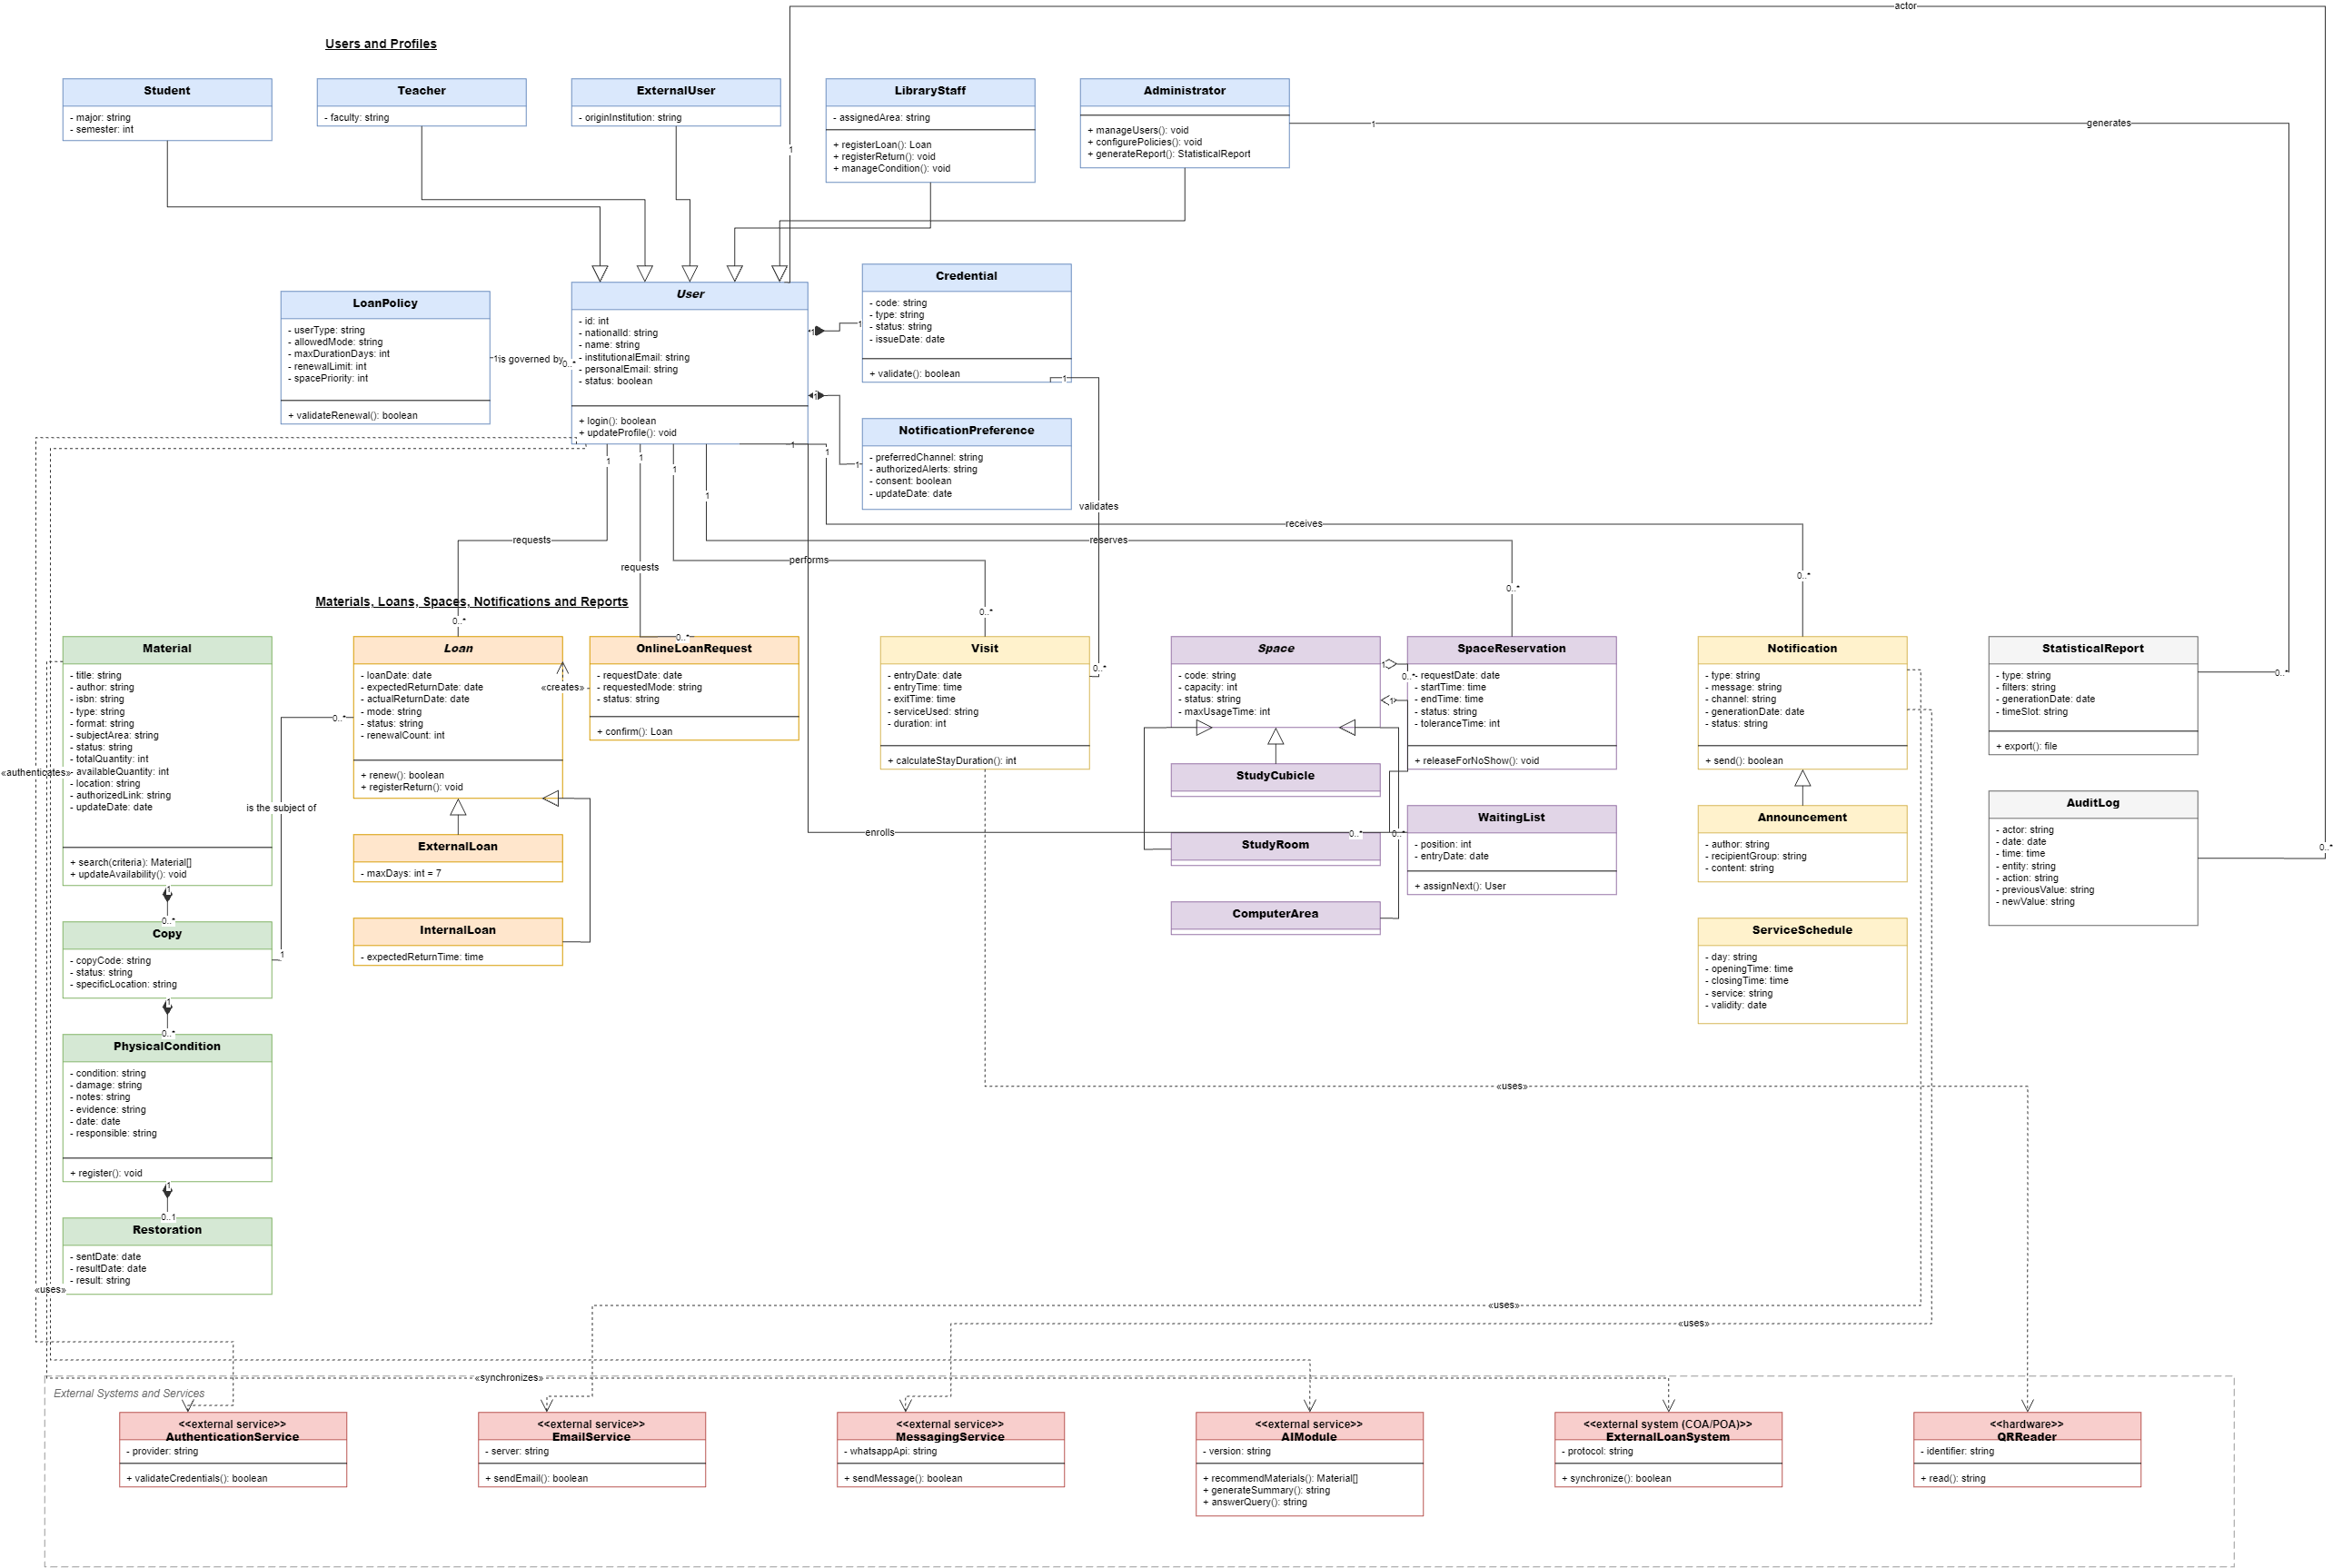
\includegraphics[height=0.78\textheight]{diagrama_clases_conceptual.png}
\caption{Diagrama de clases conceptual heredado de la Entrega 2 (1B).}
\end{figure}
\begin{figure}[H]\centering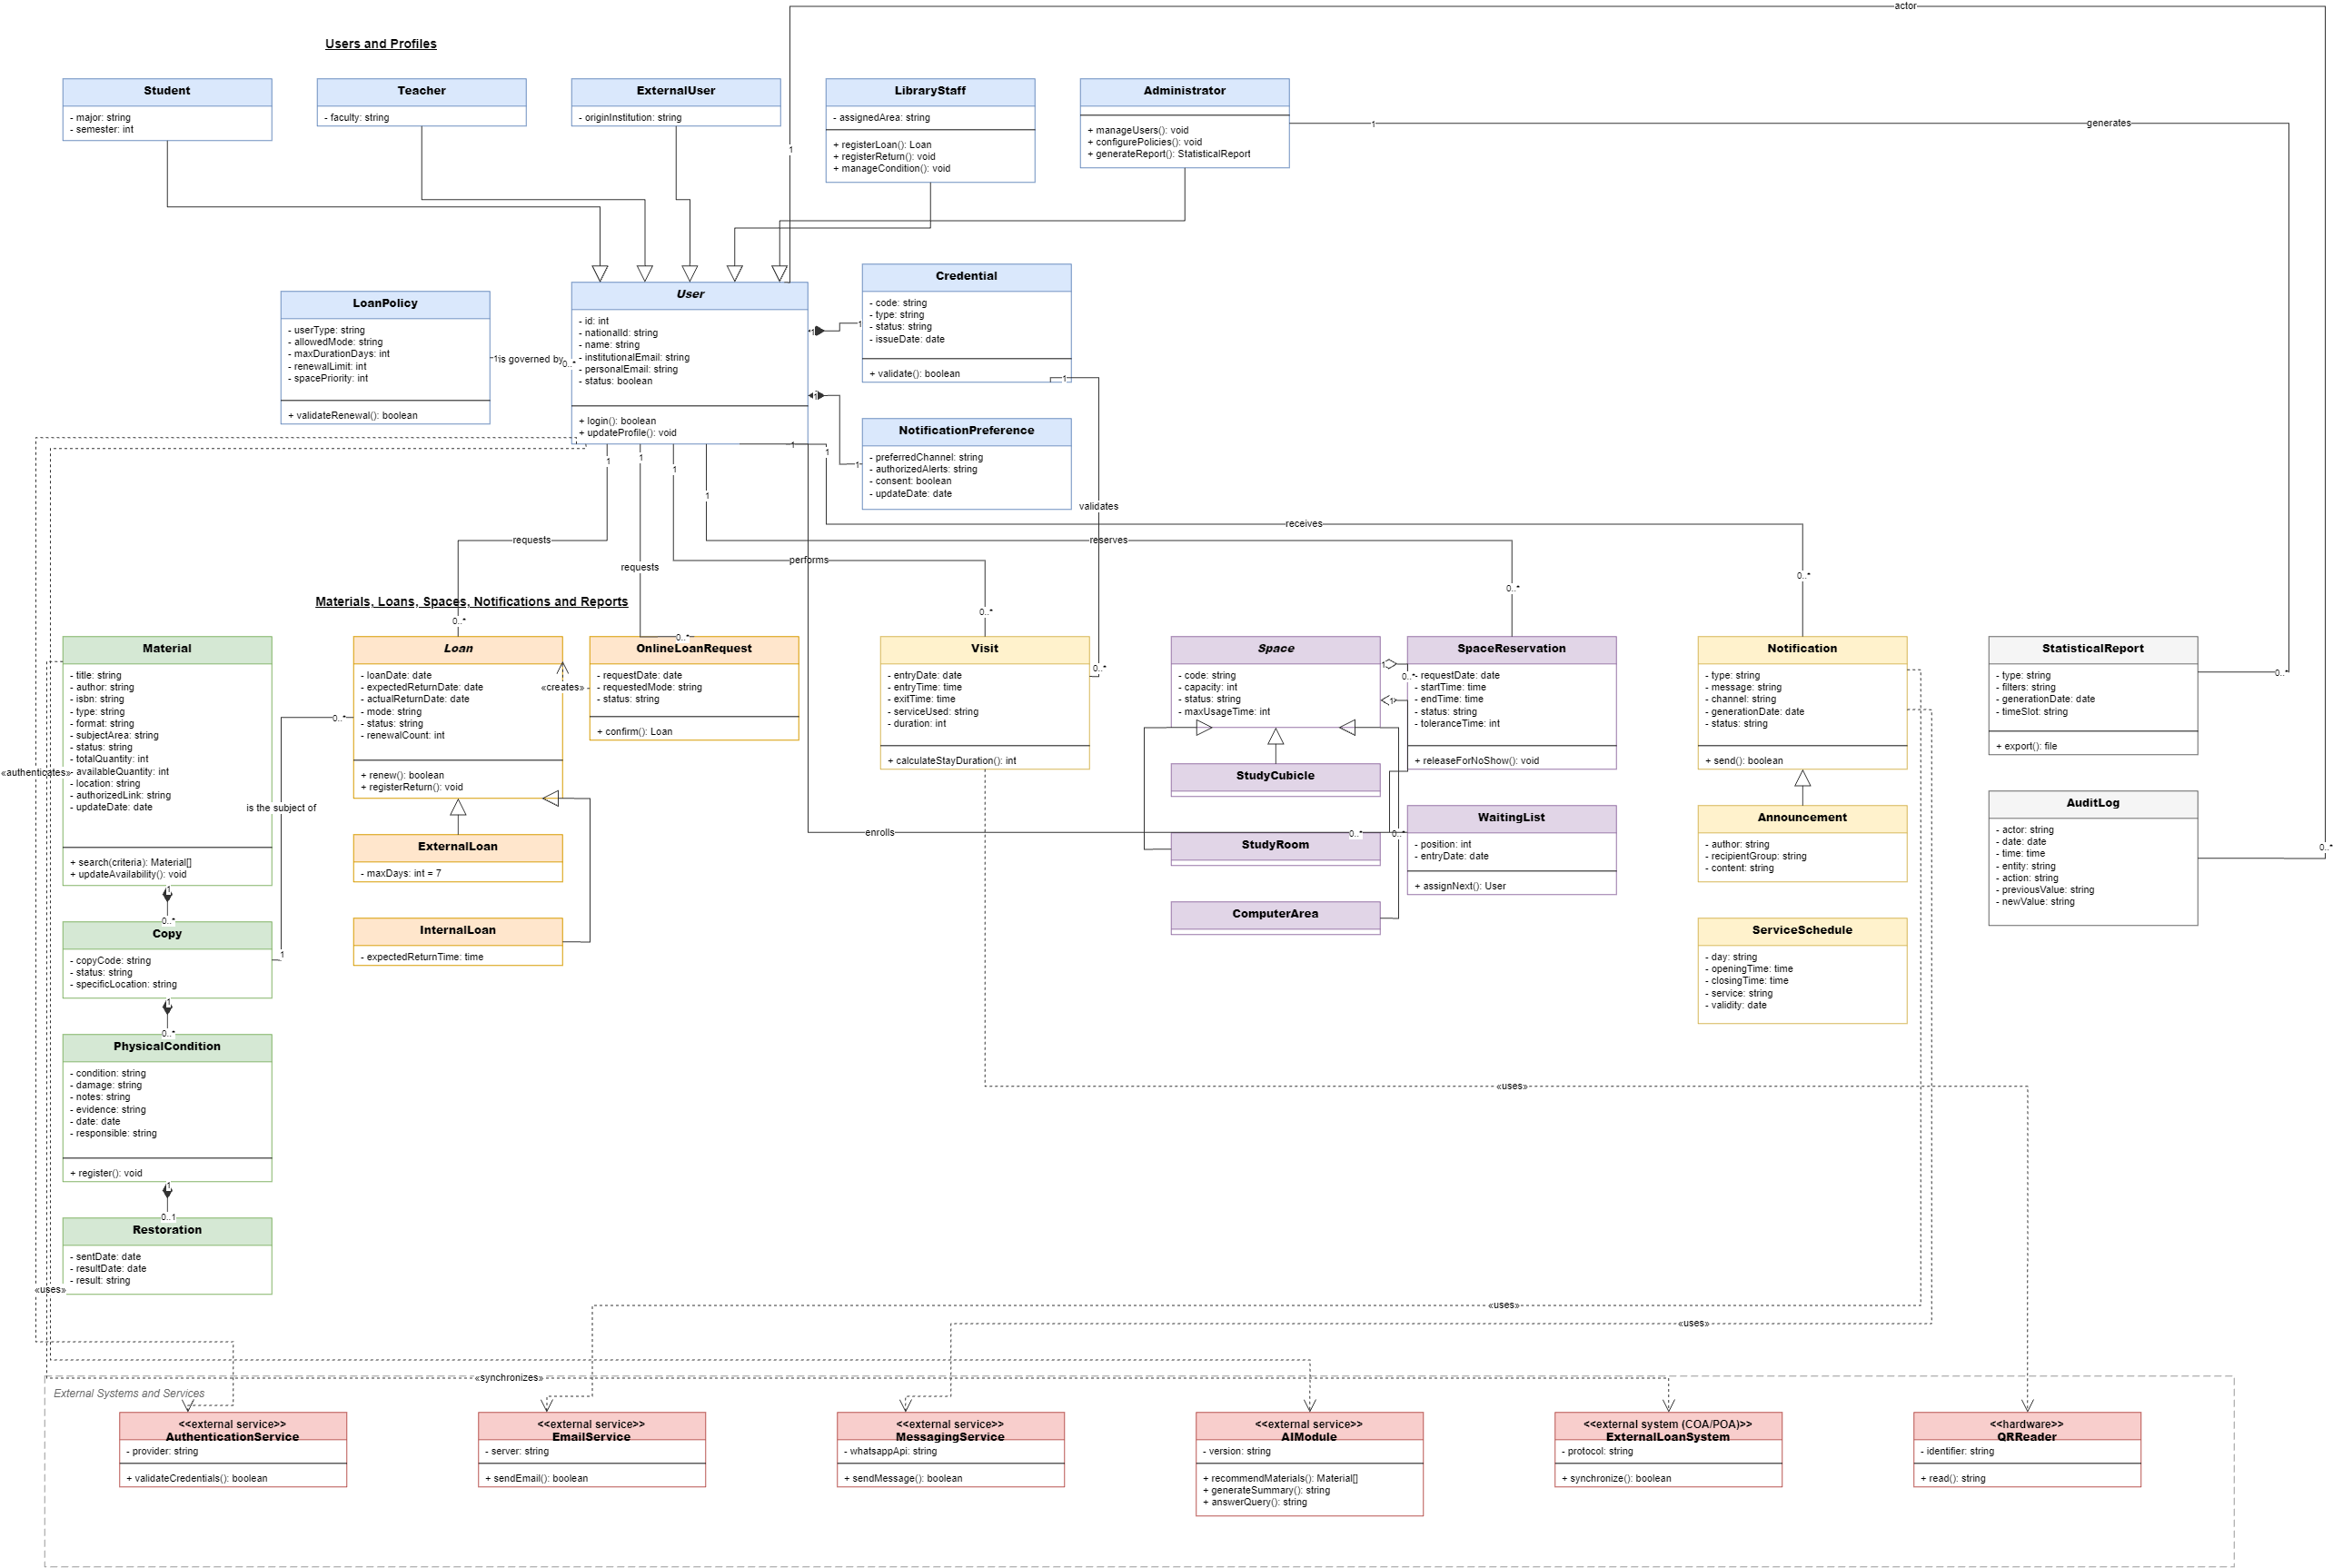
\includegraphics[width=0.95\textwidth]{diagrama_clases_conceptual.png}\caption{Diagrama de clases de SIGBUNI (atributos y relaciones; operaciones en servicios de secuencia).}\end{figure}

\subsection{Diagramas de secuencia para RF Must}
Los diagramas de secuencia de los RF Must se versionan en \path{Modelado/Diagramas_UML/secuencia/} (fuente PlantUML) y se incrustan a continuación.
\begin{longtable}{P{0.12\textwidth}P{0.20\textwidth}P{0.48\textwidth}P{0.13\textwidth}}\toprule
\textbf{ID} & \textbf{RF/CU} & \textbf{Archivo} & \textbf{Estado}\\\midrule\endfirsthead
\toprule\textbf{ID} & \textbf{RF/CU} & \textbf{Archivo} & \textbf{Estado}\\\midrule\endhead
DS-01 & RF-01 / CU-02 & \path{secuencia/DS-01_RF01_prestamo.puml} & Completo\\
DS-02 & RF-02 / CU-09 & \path{secuencia/DS-02_RF02_devolucion.puml} & Completo\\
DS-03 & RF-04 / CU-11 & \path{secuencia/DS-03_RF04_notificacion.puml} & Completo\\
DS-04 & RF-05 / CU-02 & \path{secuencia/DS-04_RF05_alerta_vencido.puml} & Completo\\
DS-05 & RF-06 / CU-01 & \path{secuencia/DS-05_RF06_catalogo.puml} & Completo\\
DS-06 & RF-07 / CU-01 & \path{secuencia/DS-06_RF07_filtros.puml} & Completo\\
DS-07 & RF-08 / CU-01 & \path{secuencia/DS-07_RF08_estado.puml} & Completo\\
DS-08 & RF-09 / CU-03 & \path{secuencia/DS-08_RF09_reserva.puml} & Completo\\
DS-09 & RF-10 / CU-03 & \path{secuencia/DS-09_RF10_disponibilidad.puml} & Completo\\
DS-10 & RF-12 / CU-04 & \path{secuencia/DS-10_RF12_ingreso.puml} & Completo\\
DS-11 & RF-13 / CU-04 & \path{secuencia/DS-11_RF13_salida.puml} & Completo\\
DS-12 & RF-17 / CU-07 & \path{secuencia/DS-12_RF17_usuarios.puml} & Completo\\
DS-13 & RF-18 / CU-06 & \path{secuencia/DS-13_RF18_reportes.puml} & Completo\\
\bottomrule\end{longtable}
\begin{figure}[H]\centering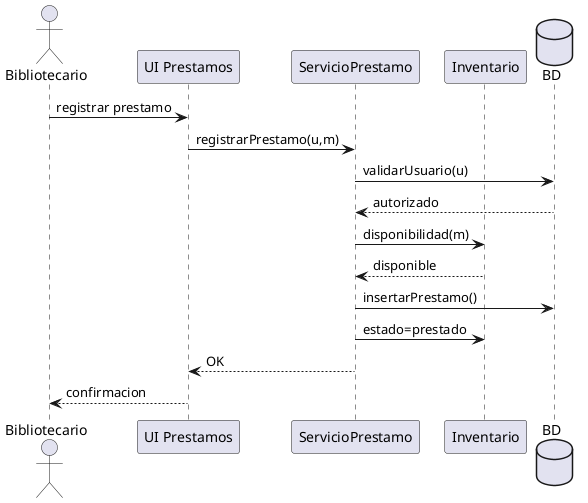
\includegraphics[width=0.88\textwidth]{DS-01_RF01_prestamo.png}\caption{DS-01: secuencia de registro de préstamo (RF-01).}\end{figure}
\begin{figure}[H]\centering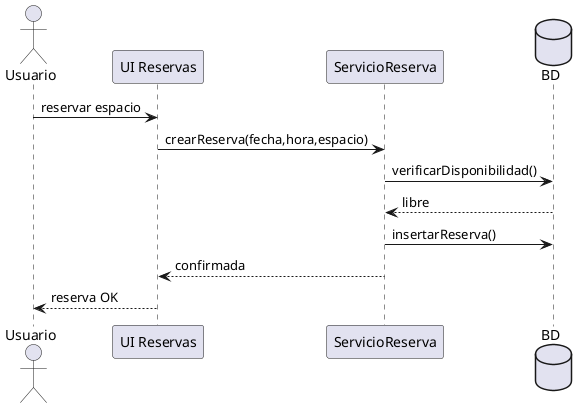
\includegraphics[width=0.88\textwidth]{DS-08_RF09_reserva.png}\caption{DS-08: secuencia de reserva de espacio (RF-09).}\end{figure}
\begin{figure}[H]\centering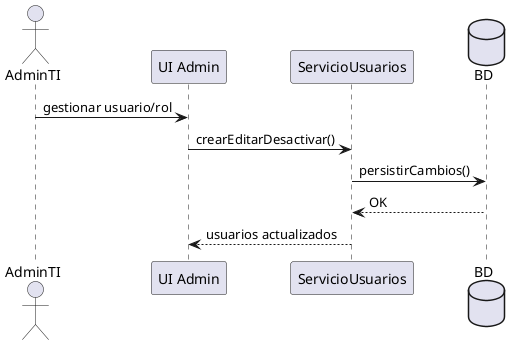
\includegraphics[width=0.88\textwidth]{DS-12_RF17_usuarios.png}\caption{DS-12: secuencia de gestión de usuarios (RF-17).}\end{figure}

\subsection{Diagramas de actividad para flujos principales}
Se documentan los flujos principales Must; el resto se deriva de los mismos patrones de control.
\begin{figure}[H]\centering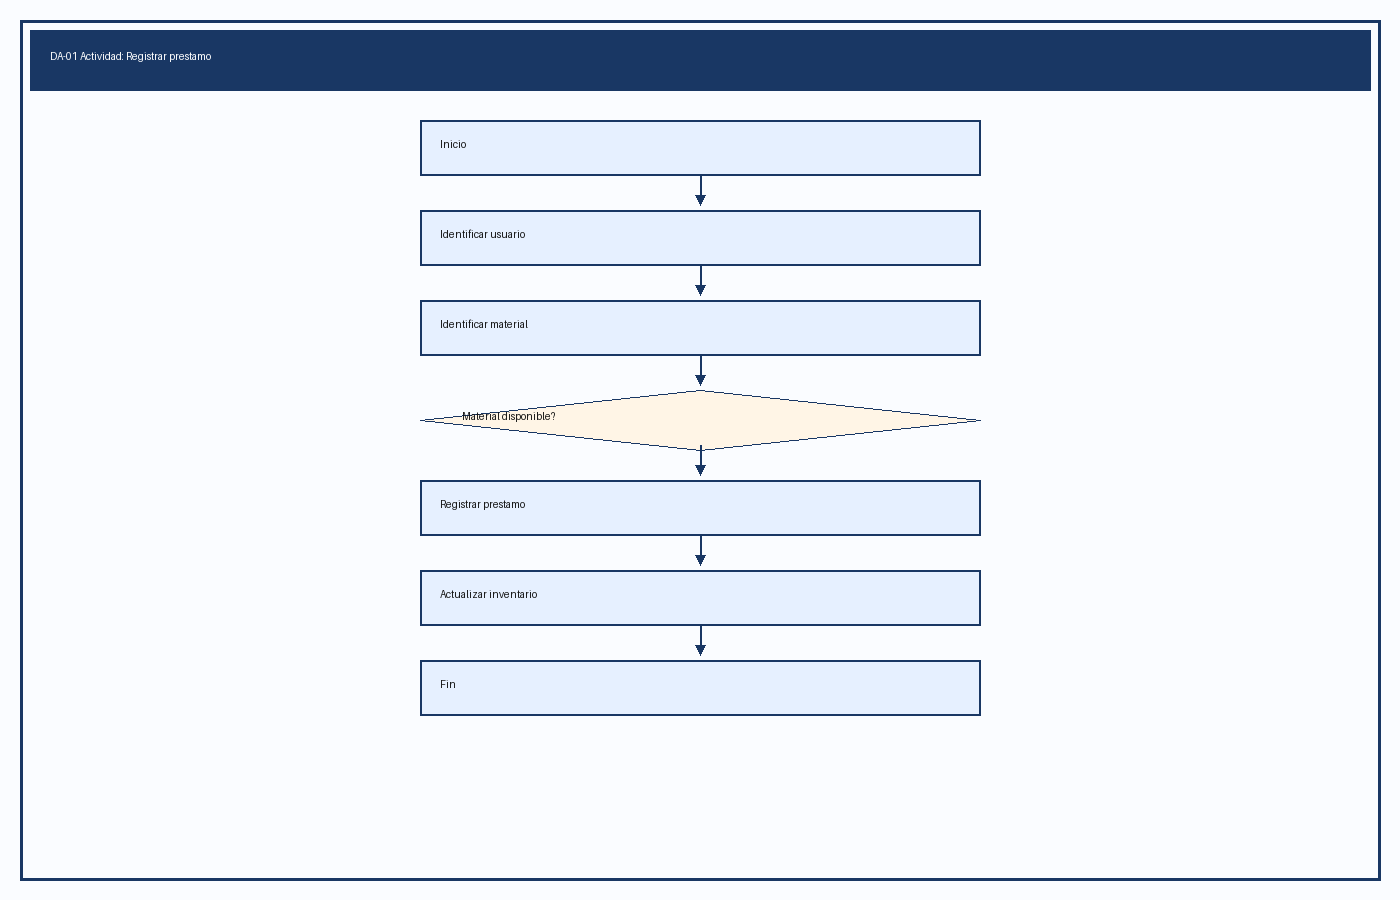
\includegraphics[width=0.85\textwidth]{DA-01_RF01_prestamo.png}\caption{DA-01: actividad de registro de préstamo.}\end{figure}
\begin{figure}[H]\centering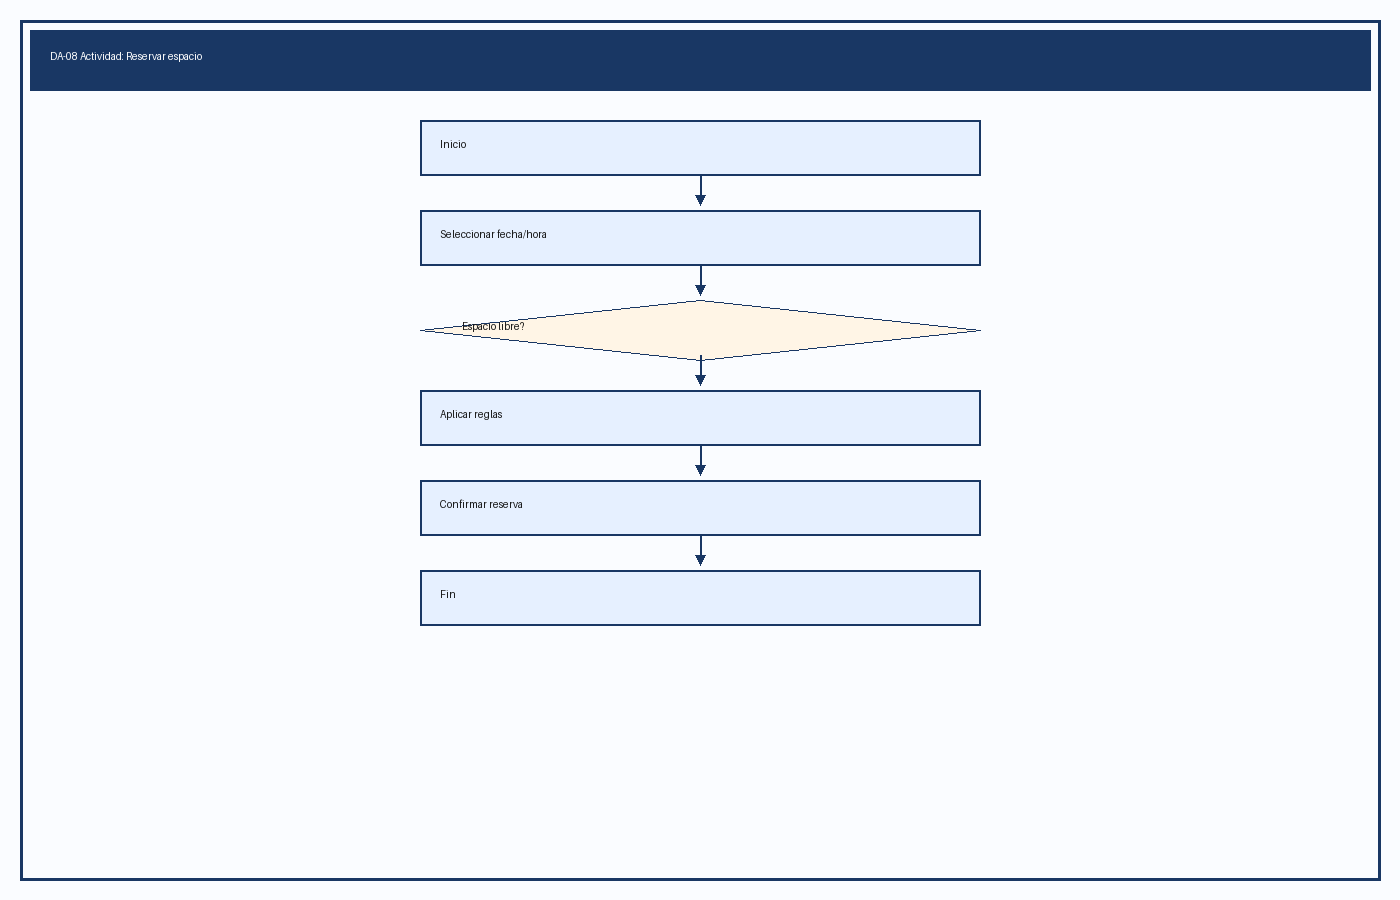
\includegraphics[width=0.85\textwidth]{DA-08_RF09_reserva.png}\caption{DA-08: actividad de reserva de espacio.}\end{figure}
\begin{figure}[H]\centering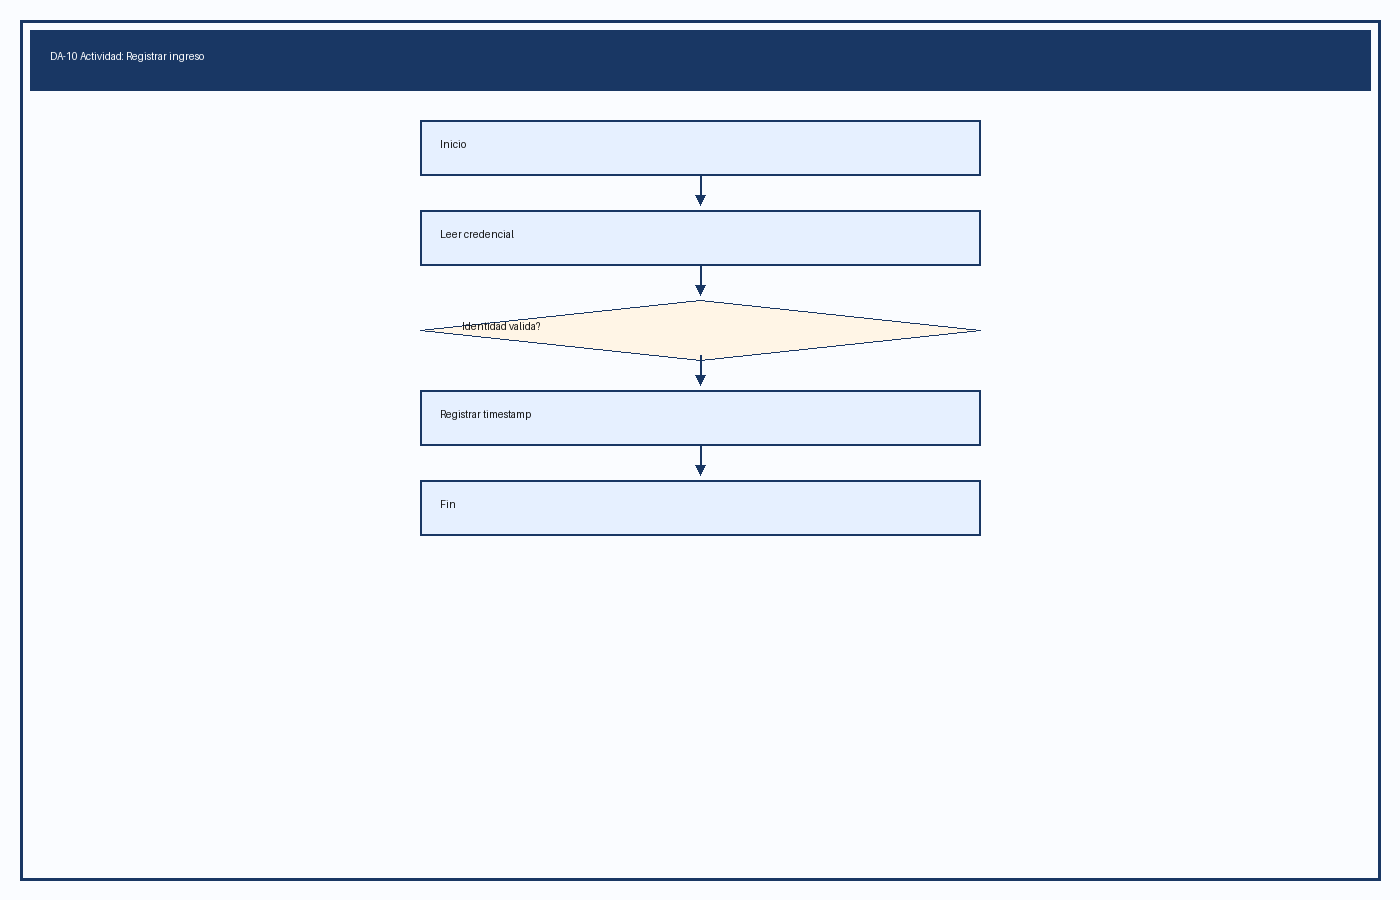
\includegraphics[width=0.85\textwidth]{DA-10_RF12_ingreso.png}\caption{DA-10: actividad de registro de ingreso.}\end{figure}
\begin{figure}[H]\centering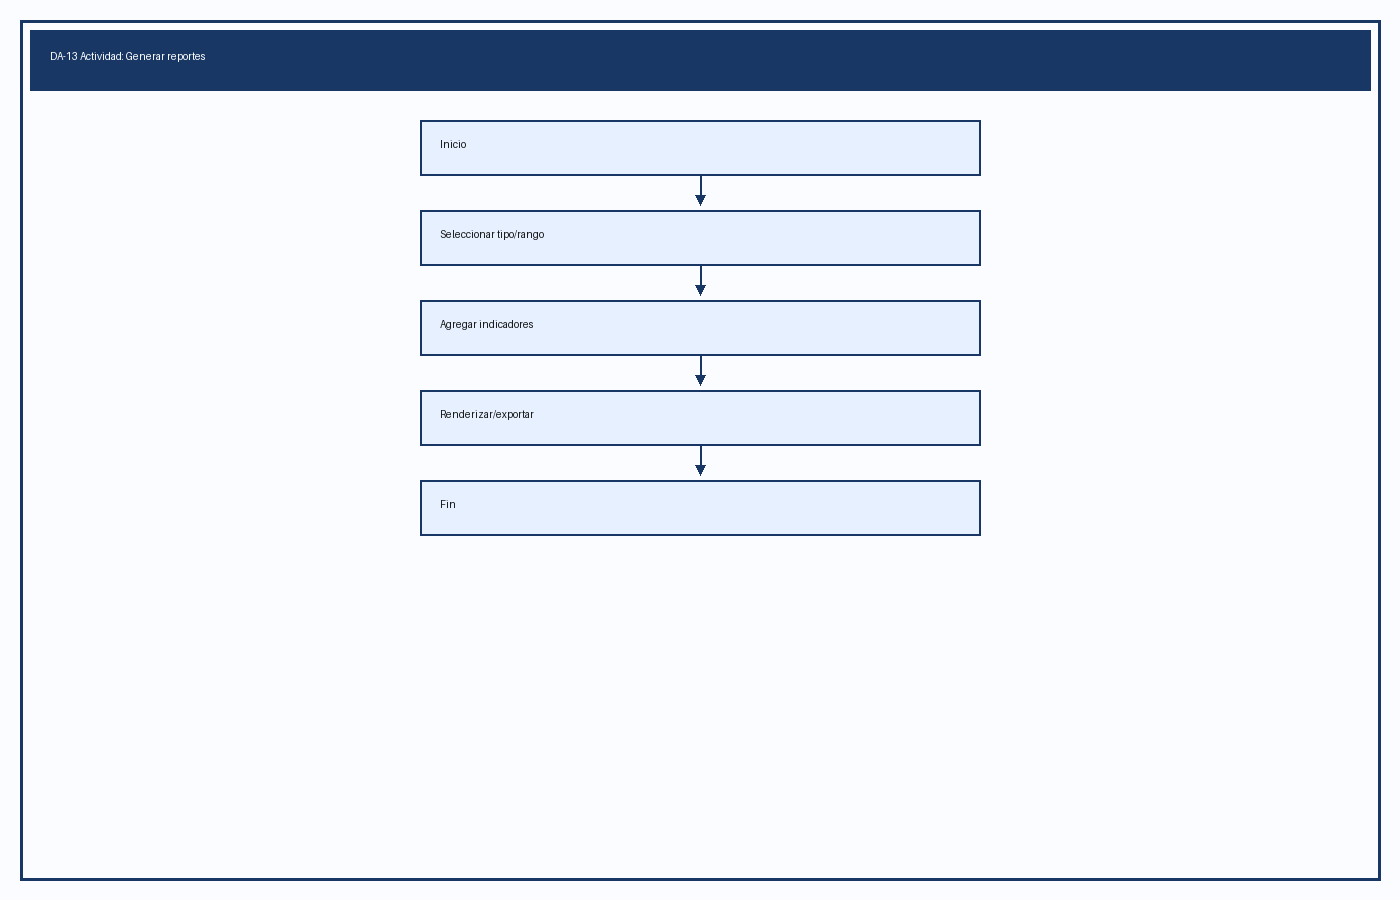
\includegraphics[width=0.85\textwidth]{DA-13_RF18_reportes.png}\caption{DA-13: actividad de generación de reportes.}\end{figure}

\subsection{Diagramas de estados}
\begin{figure}[H]\centering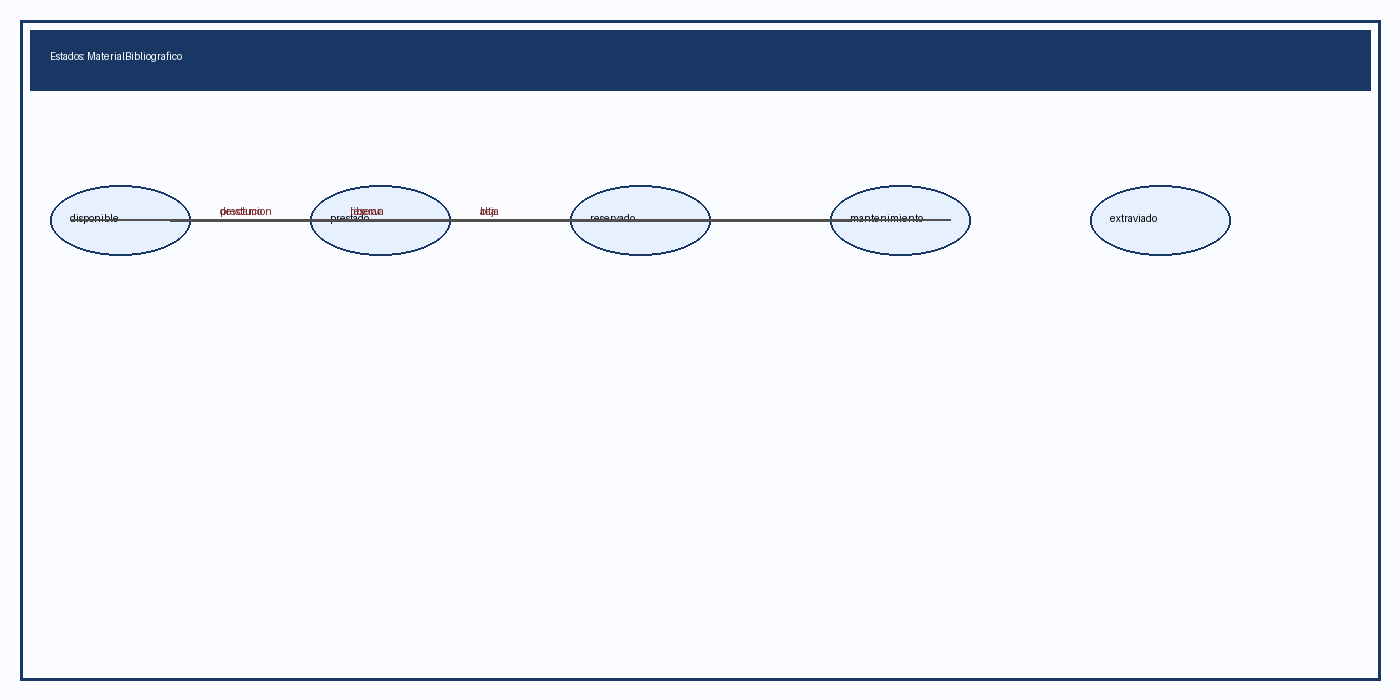
\includegraphics[width=0.92\textwidth]{EST-Material.png}\caption{Estados de MaterialBibliográfico.}\end{figure}
\begin{figure}[H]\centering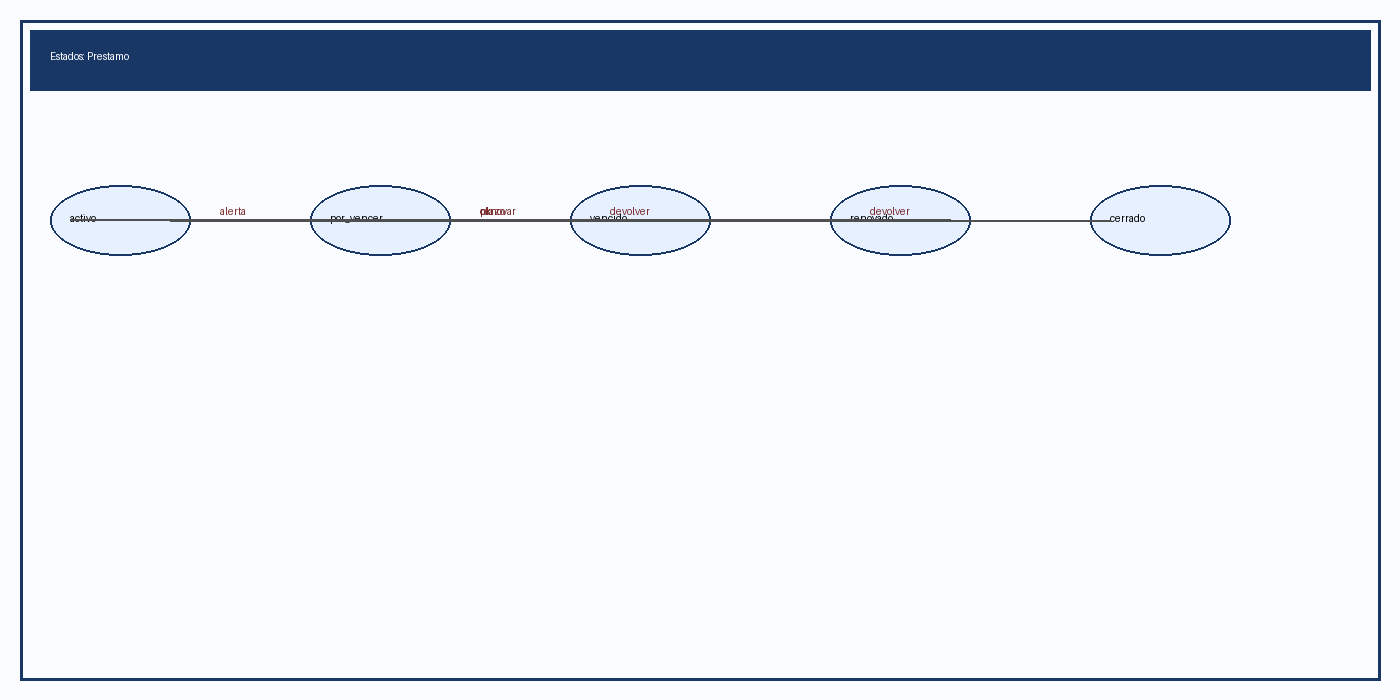
\includegraphics[width=0.92\textwidth]{EST-Prestamo.png}\caption{Estados de Préstamo.}\end{figure}
\begin{figure}[H]\centering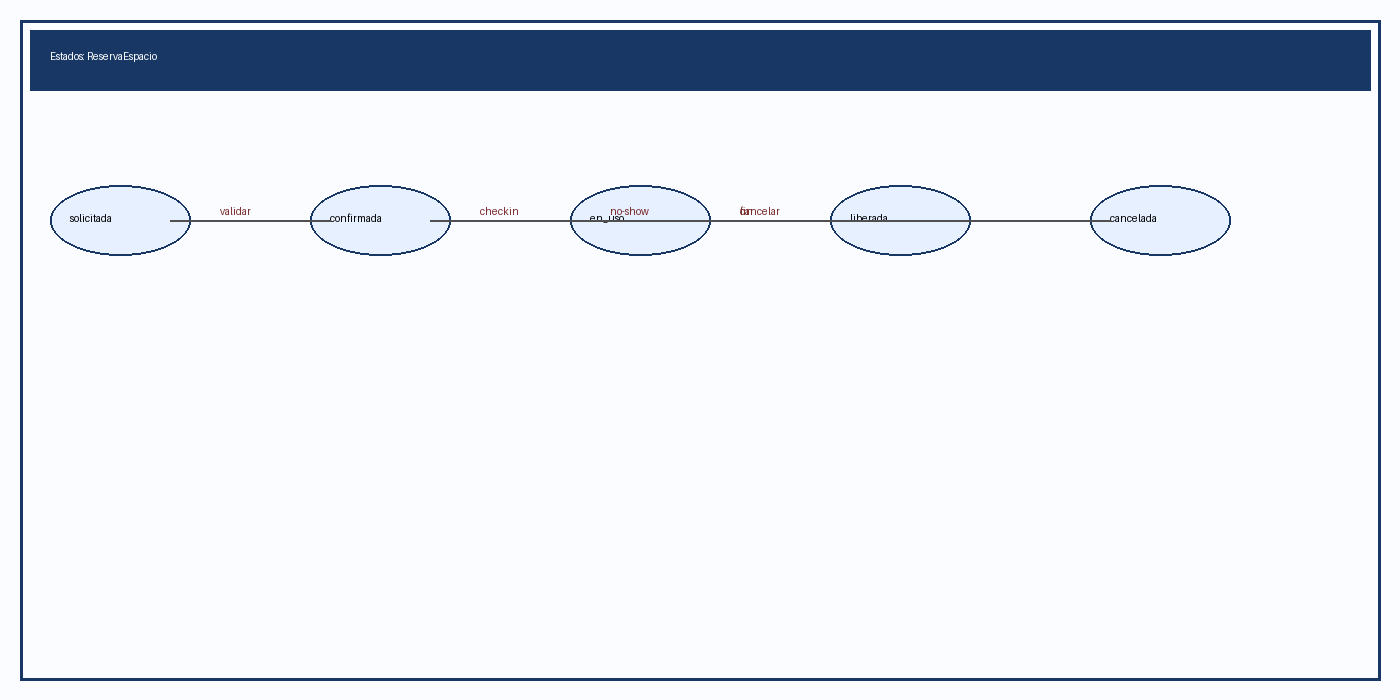
\includegraphics[width=0.92\textwidth]{EST-Reserva.png}\caption{Estados de ReservaEspacio.}\end{figure}

\subsection{Diagrama de componentes}
\begin{figure}[H]\centering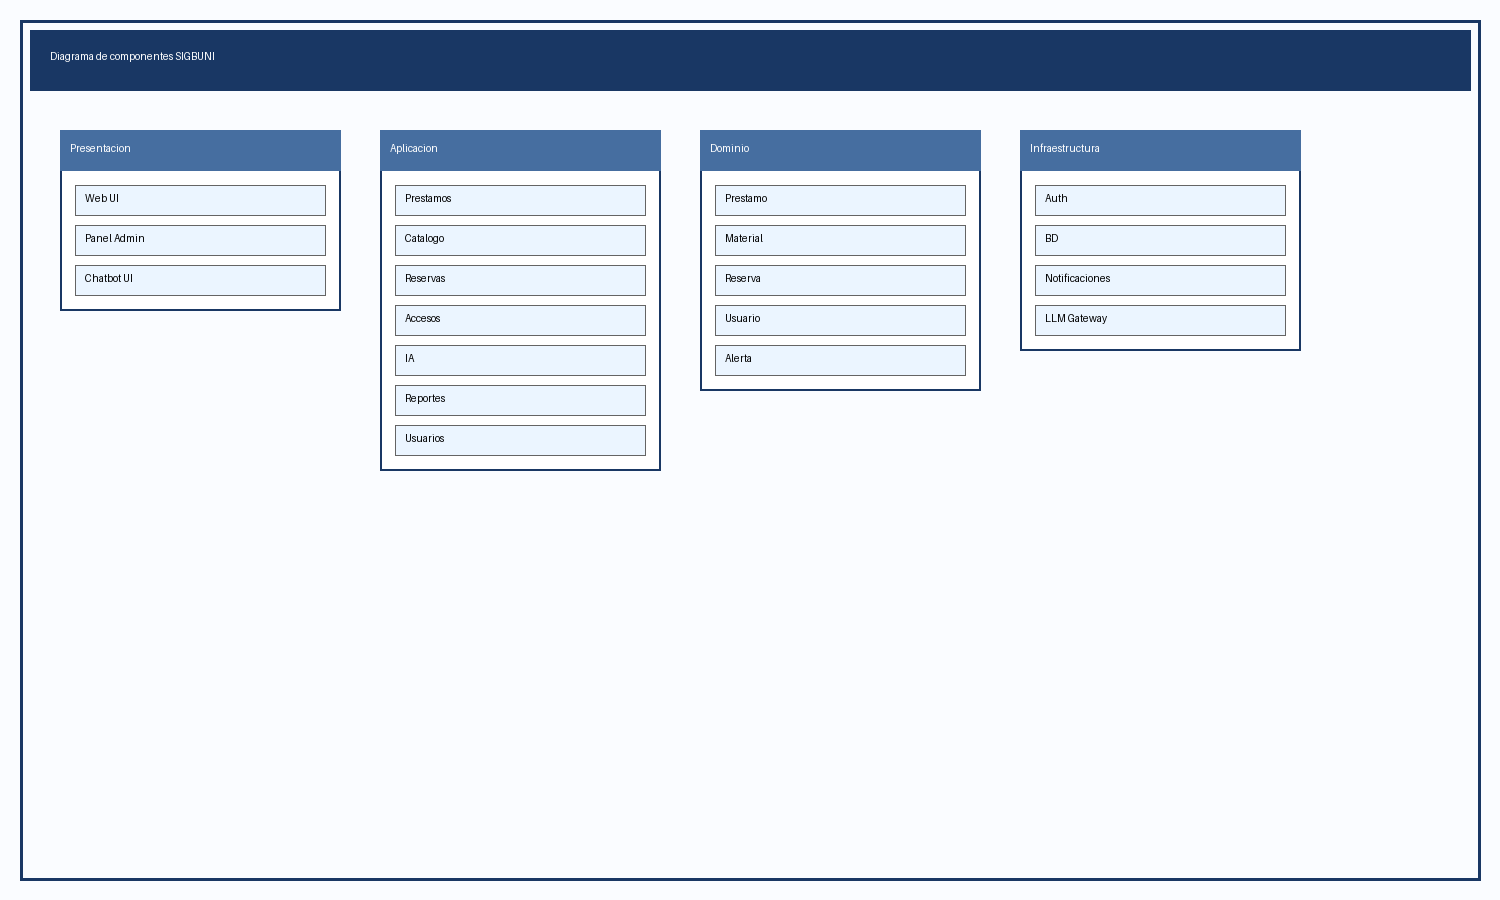
\includegraphics[width=0.95\textwidth]{CMP-componentes.png}\caption{Diagrama de componentes de SIGBUNI.}\end{figure}

\subsection{Diagrama de despliegue}
\begin{figure}[H]\centering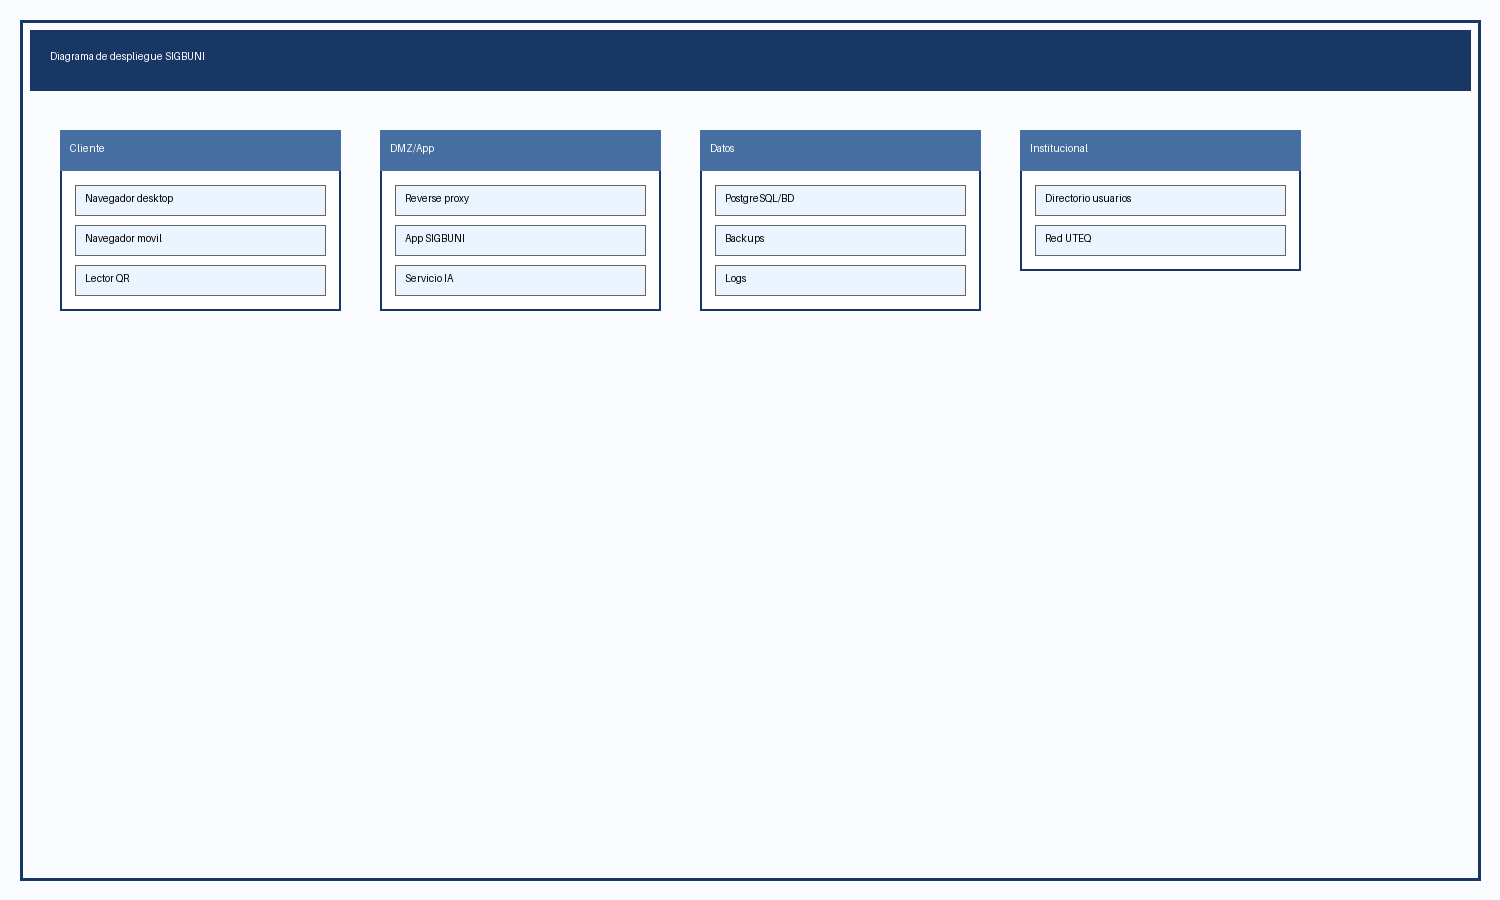
\includegraphics[width=0.95\textwidth]{DEP-despliegue.png}\caption{Diagrama de despliegue de SIGBUNI.}\end{figure}

\section{Priorización y trazabilidad extendida}
\subsection{Priorización MoSCoW, Kano y WSJF}
La clasificación MoSCoW proviene de la Entrega 2 (1B) y se extiende a RF-21--RF-25. Kano y WSJF se estiman analíticamente a partir del impacto operativo documentado en EV-01--EV-15 y de la criticidad MoSCoW; deben validarse en walkthrough. El detalle CSV está en \path{Trazabilidad/priorizacion_moscow_kano.csv}.

\begin{longtable}{P{0.10\textwidth}P{0.14\textwidth}P{0.14\textwidth}P{0.10\textwidth}P{0.42\textwidth}}\toprule
\textbf{RF} & \textbf{MoSCoW} & \textbf{Kano} & \textbf{WSJF} & \textbf{Justificación/evidencia}\\\midrule\endfirsthead
\toprule\textbf{RF} & \textbf{MoSCoW} & \textbf{Kano} & \textbf{WSJF} & \textbf{Justificación/evidencia}\\\midrule\endhead
RF-01 & Must & Basic & 4.8 & Operación crítica diaria de biblioteca (EV-01,EV-15)\\
RF-02 & Must & Basic & 5.75 & Cierra el ciclo del préstamo (EV-01)\\
RF-03 & Should & Performance & 5.0 & Reduce filas y mejora autoservicio (EV-10)\\
RF-04 & Must & Performance & 7.67 & Evita vencimientos y pérdida de material (EV-01,EV-08)\\
RF-05 & Must & Basic & 7.67 & Control operativo de morosidad (EV-01)\\
RF-06 & Must & Basic & 5.25 & Acceso al acervo es servicio base (EV-02,EV-13)\\
RF-07 & Must & Performance & 6.0 & Reduce tiempo de búsqueda (EV-02)\\
RF-08 & Must & Basic & 10.0 & Evita desplazamientos inútiles (EV-02)\\
RF-09 & Must & Performance & 4.0 & Alta demanda de espacios observada (EV-03,EV-15)\\
RF-10 & Must & Basic & 5.67 & Habilita decisión de reserva (EV-03)\\
RF-11 & Should & Performance & 4.75 & Libera espacios por inasistencia (EV-03)\\
RF-12 & Must & Basic & 5.75 & Control de aforo e ingreso (EV-04)\\
RF-13 & Must & Basic & 7.67 & Completa permanencia y aforo (EV-04)\\
RF-14 & Should & Attractive & 2.6 & Reduce carga de orientación (EV-05)\\
RF-15 & Should & Attractive & 2.5 & Apoyo académico con IA (EV-05)\\
RF-16 & Could & Attractive & 1.83 & Valor agregado, no crítico (EV-06)\\
RF-17 & Must & Basic & 5.0 & Seguridad y segregación de roles (EV-09)\\
RF-18 & Must & Performance & 4.0 & Decisiones de gestión (EV-07,EV-14)\\
RF-19 & Should & Performance & 4.0 & Comunicación masiva (EV-11)\\
RF-20 & Could & Attractive & 1.83 & Personalización dependiente de privacidad (EV-12)\\
RF-21 & Must & Basic & 6.0 & Consulta de préstamos propios (mockup MU-06) (EV-01,EV-08,EV-10)\\
RF-22 & Must & Basic & 9.33 & Puerta de autenticación institucional (EV-09)\\
RF-23 & Must & Basic & 5.0 & Inventario actualizado (panel bibliotecario) (EV-01,EV-02)\\
RF-24 & Should & Performance & 7.5 & Cancelación de reserva por usuario (EV-03)\\
RF-25 & Should & Performance & 4.75 & Aforo en horarios críticos (EV-07,EV-14)\\
\bottomrule\end{longtable}

\subsection{Matriz de trazabilidad extendida}
La matriz enlaza Ley $\rightarrow$ Objetivo $\rightarrow$ Stakeholder $\rightarrow$ EV $\rightarrow$ RF/RNF/RD $\rightarrow$ CU $\rightarrow$ HU $\rightarrow$ CA $\rightarrow$ Componente $\rightarrow$ Mockup. Se incluye el CSV reproducible en \path{Trazabilidad/matriz_trazabilidad.csv} (45 filas).

\begin{landscape}
\tiny
\begin{longtable}{P{0.9cm}P{1.5cm}P{0.8cm}P{0.8cm}P{1.3cm}P{0.9cm}P{0.7cm}P{0.8cm}P{0.8cm}P{0.8cm}P{1.1cm}P{0.9cm}P{1.0cm}}
\toprule
\textbf{ID} & \textbf{Ley/Art.} & \textbf{Obj.} & \textbf{Stake.} & \textbf{EV} & \textbf{Req.} & \textbf{Tipo} & \textbf{CU} & \textbf{HU} & \textbf{CA} & \textbf{Comp.} & \textbf{Mockup} & \textbf{Estado}\\\midrule\endfirsthead
\toprule
\textbf{ID} & \textbf{Ley/Art.} & \textbf{Obj.} & \textbf{Stake.} & \textbf{EV} & \textbf{Req.} & \textbf{Tipo} & \textbf{CU} & \textbf{HU} & \textbf{CA} & \textbf{Comp.} & \textbf{Mockup} & \textbf{Estado}\\\midrule\endhead
MT-001 & LOPDP Art.26 & OBJ-01 & S-03 & EV-01 & RF-01 & RF & CU-02 & HU-01 & CA-01 & CMP-PRE & MU-07 & Completo\\
MT-002 & LOPDP Art.26 & OBJ-01 & S-03 & EV-01 & RF-02 & RF & CU-09 & HU-02 & CA-02 & CMP-PRE & MU-07 & Completo\\
MT-003 & LOPDP Art.7 & OBJ-01 & S-01 & EV-10 & RF-03 & RF & CU-02 & HU-03 & CA-03 & CMP-PRE & MU-06 & Completo\\
MT-004 & LOPDP Art.26 & OBJ-01 & S-01 & EV-01/08 & RF-04 & RF & CU-02 & HU-04 & CA-04 & CMP-NOT & MU-06 & Completo\\
MT-005 & LOPDP Art.26 & OBJ-01 & S-03 & EV-01 & RF-05 & RF & CU-02 & HU-05 & CA-05 & CMP-NOT & MU-05 & Completo\\
MT-006 & LOPDP Art.14 & OBJ-04 & S-01 & EV-02/13 & RF-06 & RF & CU-01 & HU-06 & CA-06 & CMP-CAT & MU-02 & Completo\\
MT-007 & LOPDP Art.14 & OBJ-04 & S-01 & EV-02 & RF-07 & RF & CU-01 & HU-07 & CA-07 & CMP-CAT & MU-02 & Completo\\
MT-008 & LOPDP Art.14 & OBJ-04 & S-01 & EV-02 & RF-08 & RF & CU-01 & HU-08 & CA-08 & CMP-CAT & MU-02 & Completo\\
MT-009 & LOPDP Art.7 & OBJ-02 & S-01 & EV-03/15 & RF-09 & RF & CU-03 & HU-09 & CA-09 & CMP-RES & MU-03 & Completo\\
MT-010 & LOPDP Art.7 & OBJ-02 & S-01 & EV-03 & RF-10 & RF & CU-03 & HU-10 & CA-10 & CMP-RES & MU-03 & Completo\\
MT-011 & LOPDP Art.7 & OBJ-02 & S-03 & EV-03 & RF-11 & RF & CU-03 & HU-11 & CA-11 & CMP-RES & MU-03 & Completo\\
MT-012 & LOPDP Art.12 & OBJ-03 & S-03 & EV-04 & RF-12 & RF & CU-04 & HU-12 & CA-12 & CMP-ACC & MU-05 & Completo\\
MT-013 & LOPDP Art.12 & OBJ-03 & S-03 & EV-04 & RF-13 & RF & CU-04 & HU-13 & CA-13 & CMP-ACC & MU-05 & Completo\\
MT-014 & LOPDP Art.8 & OBJ-05 & S-01 & EV-05 & RF-14 & RF & CU-05 & HU-14 & CA-14 & CMP-IA & MU-04 & Completo\\
MT-015 & LOPDP Art.8 & OBJ-05 & S-01 & EV-05 & RF-15 & RF & CU-05 & HU-15 & CA-15 & CMP-IA & MU-04 & Completo\\
MT-016 & LOPDP Art.8 & OBJ-05 & S-01 & EV-06 & RF-16 & RF & CU-05 & HU-16 & CA-16 & CMP-IA & MU-04 & Completo\\
MT-017 & LOPDP Art.26 & OBJ-06 & S-05 & EV-09 & RF-17 & RF & CU-07 & HU-17 & CA-17 & CMP-ADM & MU-08 & Completo\\
MT-018 & LOPDP Art.14 & OBJ-06 & S-04 & EV-07/14 & RF-18 & RF & CU-06 & HU-18 & CA-18 & CMP-REP & MU-05 & Completo\\
MT-019 & LOPDP Art.7 & OBJ-06 & S-03 & EV-11 & RF-19 & RF & CU-08 & HU-19 & CA-19 & CMP-NOT & MU-05 & Completo\\
MT-020 & LOPDP Art.8 & OBJ-05 & S-01 & EV-12 & RF-20 & RF & CU-05 & HU-20 & CA-20 & CMP-IA & MU-04 & Completo\\
MT-021 & LOPDP Art.14 & OBJ-01 & S-01 & EV-01/08/10 & RF-21 & RF & CU-11 & HU-21 & CA-21 & CMP-PRE & MU-06 & Completo\\
MT-022 & LOPDP Art.26 & OBJ-06 & S-05 & EV-09 & RF-22 & RF & CU-12 & HU-22 & CA-22 & CMP-ADM & MU-01 & Completo\\
MT-023 & LOPDP Art.26 & OBJ-04 & S-03 & EV-01/02 & RF-23 & RF & CU-13 & HU-23 & CA-23 & CMP-CAT & MU-05 & Completo\\
MT-024 & LOPDP Art.7 & OBJ-02 & S-01 & EV-03 & RF-24 & RF & CU-03 & HU-24 & CA-24 & CMP-RES & MU-03 & Completo\\
MT-025 & LOPDP Art.12 & OBJ-03 & S-04 & EV-07/14 & RF-25 & RF & CU-06 & HU-25 & CA-25 & CMP-ACC & MU-05 & Completo\\
MT-026 & ISO25010 & OBJ-04 & S-01 & EV-02 & RNF-01 & RNF & CU-01 & HU-06 & CA-06 & CMP-CAT & MU-02 & Completo\\
MT-027 & ISO25010 & OBJ-06 & S-05 & EV-09 & RNF-02 & RNF & CU-12 & -- & -- & CMP-ADM & MU-01 & Completo\\
MT-028 & LOPDP Art.26 & OBJ-06 & S-05 & EV-09 & RNF-03 & RNF & CU-12 & HU-22 & CA-22 & CMP-ADM & MU-01 & Completo\\
MT-029 & ISO25010 & OBJ-02 & S-01 & EV-03 & RNF-04 & RNF & CU-03 & HU-09 & CA-09 & CMP-RES & MU-03 & Completo\\
MT-030 & ISO25010 & OBJ-04 & S-01 & EV-13 & RNF-05 & RNF & CU-01 & HU-06 & CA-06 & CMP-CAT & MU-02 & Completo\\
MT-031 & ISO25010 & OBJ-01 & S-03 & EV-01 & RNF-06 & RNF & CU-02 & HU-01 & CA-01 & CMP-PRE & MU-07 & Completo\\
MT-032 & ISO25010 & OBJ-06 & S-05 & EV-09 & RNF-07 & RNF & CU-07 & HU-17 & CA-17 & CMP-ADM & MU-09 & Completo\\
MT-033 & LOPDP Art.26 & OBJ-06 & S-05 & EV-09 & RNF-08 & RNF & CU-07 & HU-17 & CA-17 & CMP-ADM & MU-08 & Completo\\
MT-034 & ISO25010 & OBJ-01 & S-03 & EV-01 & RNF-09 & RNF & CU-02 & HU-01 & CA-01 & CMP-PRE & MU-07 & Completo\\
MT-035 & ISO25010 & OBJ-06 & S-05 & EV-09 & RNF-10 & RNF & CU-12 & -- & -- & CMP-ADM & MU-09 & Completo\\
MT-036 & ISO25010 & OBJ-06 & S-05 & EV-09 & RNF-11 & RNF & CU-07 & HU-17 & CA-17 & CMP-ADM & MU-09 & Completo\\
MT-037 & LOPDP Art.8 & OBJ-05 & S-01 & EV-05 & RNF-12 & RNF & CU-05 & HU-15 & CA-15 & CMP-IA & MU-04 & Completo\\
MT-038 & LOPDP Art.8 & OBJ-05 & S-01 & EV-06 & RNF-13 & RNF & CU-05 & HU-16 & CA-16 & CMP-IA & MU-04 & Completo\\
MT-039 & LOPDP Art.8 & OBJ-05 & S-01 & EV-05 & RNF-14 & RNF & CU-05 & HU-14 & CA-14 & CMP-IA & MU-04 & Completo\\
MT-040 & LOPDP Art.26 & OBJ-06 & S-05 & EV-09 & RNF-15 & RNF & CU-07 & HU-17 & CA-17 & CMP-ADM & MU-08 & Completo\\
MT-041 & RD & OBJ-06 & S-05 & EV-09 & RD-01 & RD & CU-12 & HU-22 & CA-22 & CMP-ADM & MU-01 & Completo\\
MT-042 & RD & OBJ-01 & S-03 & EV-01 & RD-02 & RD & CU-02 & HU-01 & CA-01 & CMP-PRE & MU-07 & Completo\\
MT-043 & RD & OBJ-04 & S-01 & EV-02 & RD-03 & RD & CU-01 & HU-06 & CA-06 & CMP-CAT & MU-02 & Completo\\
MT-044 & LOPDP Art.26 & OBJ-06 & S-05 & EV-09 & RD-04 & RD & CU-07 & HU-17 & CA-17 & CMP-ADM & MU-08 & Completo\\
MT-045 & RD & OBJ-03 & S-03 & EV-04 & RD-05 & RD & CU-04 & HU-12 & CA-12 & CMP-ACC & MU-05 & Completo\\
\bottomrule
\end{longtable}
\normalsize
\end{landscape}

\section{Producto Mínimo Viable funcional}
\subsection{Repositorio y alcance}
\textbf{Repositorio Git separado del MVP:} aún no publicado; documentar URL y commit evaluado en \path{MVP/README.md}.\\
\textbf{Tecnologías y arquitectura propuestas:} aplicación web responsiva, API modular, base de datos relacional y gateway de IA; stack concreto pendiente de fijar en el repo del MVP.\\
\textbf{README de despliegue:} plantilla en \path{MVP/README.md}; debe incluir \texttt{docker compose up} o equivalente antes del corte.

\subsection{Cobertura de RF Must}
\begin{longtable}{P{0.10\textwidth}P{0.36\textwidth}P{0.18\textwidth}P{0.28\textwidth}}\toprule
\textbf{RF} & \textbf{Funcionalidad} & \textbf{Implementado} & \textbf{Evidencia}\\\midrule\endfirsthead
\toprule\textbf{RF} & \textbf{Funcionalidad} & \textbf{Implementado} & \textbf{Evidencia}\\\midrule\endhead
RF-01 & Registrar préstamo bibliográfico & No & Pendiente MVP\\
RF-02 & Registrar devolución de material & No & Pendiente MVP\\
RF-04 & Enviar notificación de vencimiento & No & Pendiente MVP\\
RF-05 & Generar alerta por material vencido & No & Pendiente MVP\\
RF-06 & Consultar catálogo digital & No & Pendiente MVP\\
RF-07 & Buscar material por filtros & No & Pendiente MVP\\
RF-08 & Mostrar estado del material & No & Pendiente MVP\\
RF-09 & Reservar espacio bibliotecario & No & Pendiente MVP\\
RF-10 & Mostrar disponibilidad de espacios & No & Pendiente MVP\\
RF-12 & Registrar ingreso a biblioteca & No & Pendiente MVP\\
RF-13 & Registrar salida de biblioteca & No & Pendiente MVP\\
RF-17 & Gestionar usuarios, roles y permisos & No & Pendiente MVP\\
RF-18 & Generar reportes estadísticos & No & Pendiente MVP\\
RF-21 & Consultar mis préstamos & No & Pendiente MVP\\
RF-22 & Autenticar usuario institucional & No & Pendiente MVP\\
RF-23 & Registrar y actualizar inventario & No & Pendiente MVP\\
\bottomrule\end{longtable}
\textbf{Cobertura calculada:} $0/16 = 0\%$ de RF Must (se requiere $\geq 60\%$ en código ejecutable). El estado se declara honestamente para no disparar G4.

\subsection{Demostración funcional}
\textbf{Video $\leq$ 3 minutos:} pendiente en \path{MVP/video_demo.mp4}.\\
\textbf{Capturas:} se usarán capturas del MVP real; los mockups Visily no sustituyen la demostración ejecutable.

\section{Trabajo de campo extendido y validación}
\subsection{Inventario mínimo de evidencias}
\begin{longtable}{P{0.25\textwidth}P{0.18\textwidth}P{0.30\textwidth}P{0.20\textwidth}}\toprule
\textbf{Evidencia} & \textbf{Mínimo del corte} & \textbf{Ubicación} & \textbf{Estado verificado}\\\midrule\endfirsthead
\toprule\textbf{Evidencia} & \textbf{Mínimo del corte} & \textbf{Ubicación} & \textbf{Estado verificado}\\\midrule\endhead
Consentimientos firmados & $\geq 8$ para C7; avance hacia 16 & \path{Evidencias/Consentimiento/} & 10 PDF verificables (9 estudiantes + 1 bibliotecaria)\\
Videos de entrevistas & $\geq 6$ para C7; avance hacia 16 & \path{Evidencias/Video/} & 0 en repo (pendiente segunda ronda)\\
Audios redundantes & $\geq 6$ para C7; avance hacia 16 & \path{Evidencias/Audio/} & 1 audio H.264/MP3 ($\approx$7{,}5 min; personal biblioteca)\\
Fotos del entorno & $\geq 15$ para C7; meta extendida 20 & \path{Evidencias/Fotos_Entorno/} & Referencia EV-15 documental; faltan $\geq$15 fotos fechadas\\
Fotos de aplicación del cuestionario & $\geq 5$ & \path{Evidencias/Cuestionario/Fotos_Aplicacion/} & Pendiente espejo local\\
Respuestas del cuestionario & $n\geq 30$ para gatekeeper; meta $n\geq 60$ por perfil & \path{Evidencias/Cuestionario/Respuestas/} & PDF manuscrito presente; exportar CSV/XLSX\\
Documentos de la organización & $\geq 3$ para C7; meta 5 & \path{Evidencias/Documentos_Organizacion/} & Pendiente\\
Walkthrough de validación & $\geq 3$ para C7; meta 6 & \path{Evidencias/Validacion_Walkthrough/} & Pendiente\\
Codificación temática y saturación & Tabla completa + curva & \path{Evidencias/Codificacion_Tematica/} & Baseline documental EV-01--EV-15 + curva preliminar\\\bottomrule
\end{longtable}

\subsection{Evidencia heredada documentada}
Las Entregas previas muestran trabajo de campo y registran entrevistas, encuesta y fotografías. Estas imágenes se incluyen solo como referencia histórica; no sustituyen los nuevos consentimientos ni la segunda ronda requerida.
\begin{figure}[H]\centering
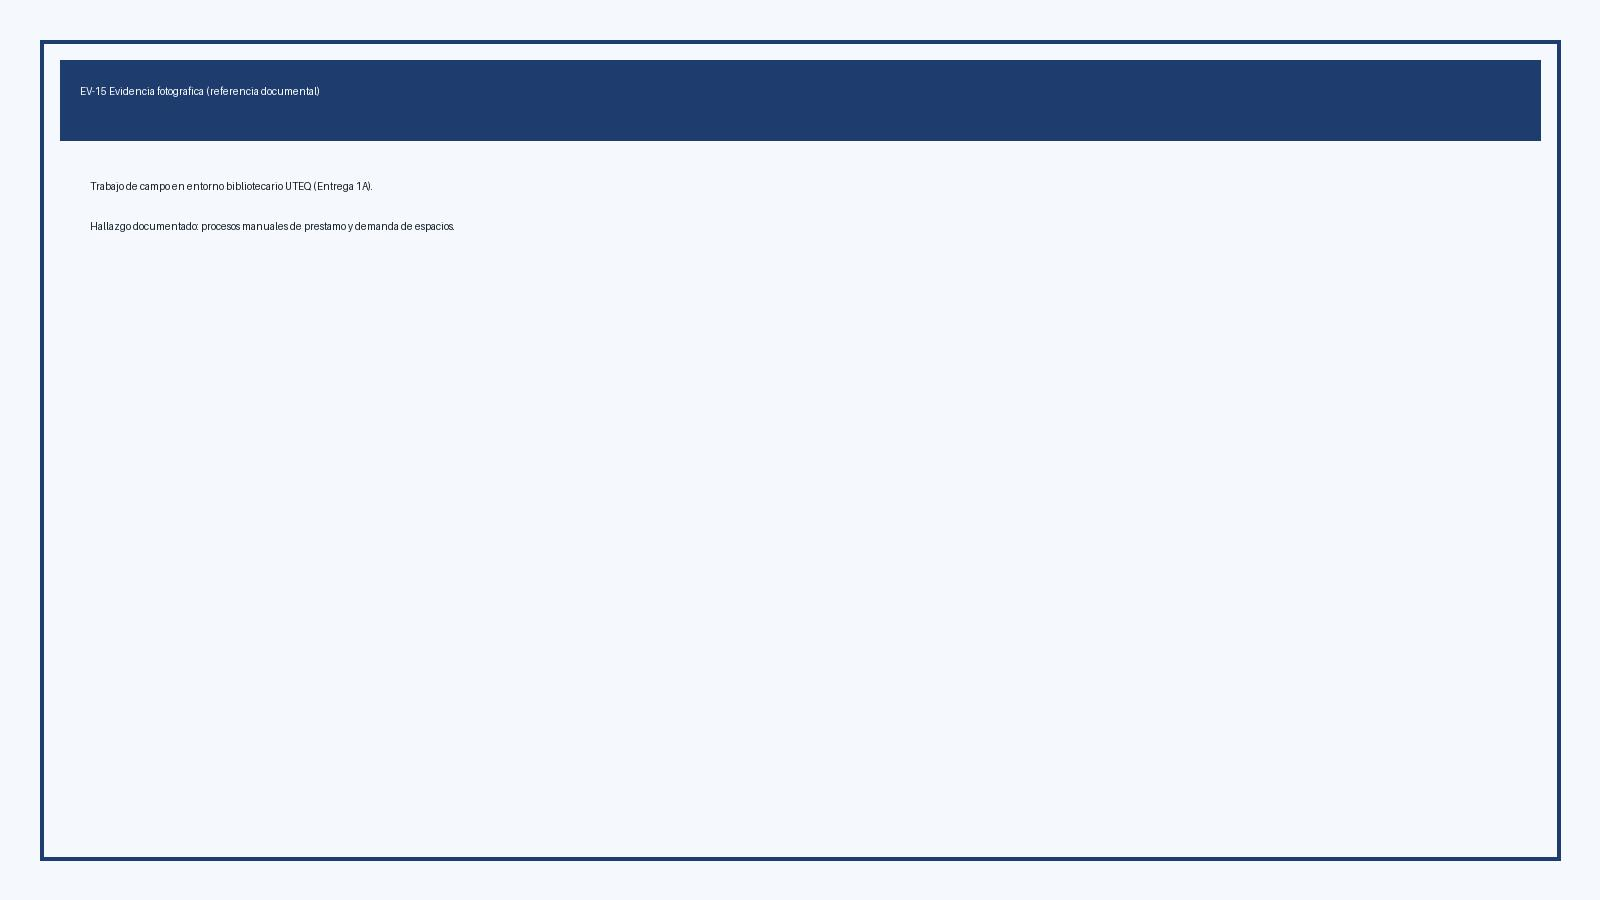
\includegraphics[height=0.42\textheight]{EV-15_trabajo_campo_01.jpg}\hfill
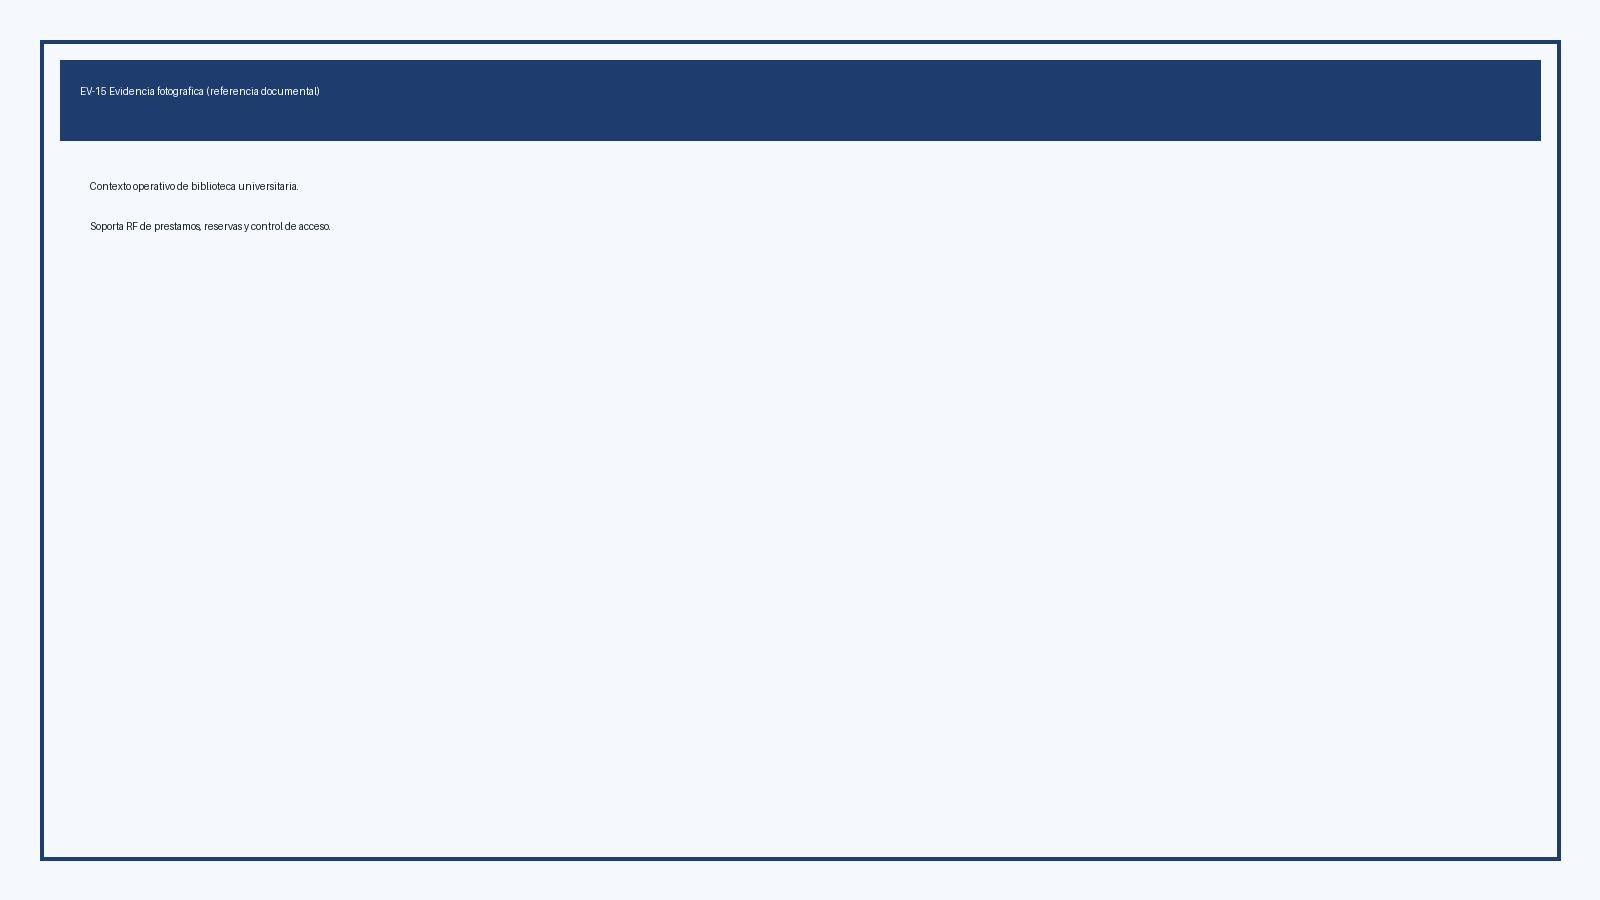
\includegraphics[height=0.42\textheight]{EV-15_trabajo_campo_02.jpg}
\caption{Evidencia fotográfica heredada de la Entrega 1A (EV-15).}
\end{figure}

\subsection{Segunda ronda de elicitación}
\textbf{Participantes y perfiles (línea base verificada):} 9 estudiantes (encuesta) + 1 personal bibliotecario (entrevista); faltan perfiles docentes, TI y directivos para alcanzar $\geq$16.\\
\textbf{Guion de entrevista v2.0:} plantilla en \path{Experimento/Instrumentos/} (ampliar con preguntas de explicabilidad IA).\\
\textbf{Cuestionario v2.0:} resultados manuscritos en \path{Evidencias/Cuestionario/Respuestas/}; se requiere exportación CSV/XLSX.\\
\textbf{Criterios de inclusión:} comunidad UTEQ usuaria o operadora de biblioteca; exclusión: menores de edad y personas sin consentimiento firmado.\\
\textbf{Consentimiento actualizado:} los consentimientos existentes cubren encuesta/entrevista; debe añadirse cláusula explícita de publicación anonimizada revisada por pares antes de OSF/Zenodo.

\subsection{Validación walkthrough}
Las sesiones VW-01--VW-06 están planificadas (3 técnicas + 3 no técnicas) y aún no tienen acta/video en el repositorio. Hasta registrarlas, no se declara cumplimiento de C7 en este subcriterio.
\begin{longtable}{P{0.12\textwidth}P{0.22\textwidth}P{0.18\textwidth}P{0.22\textwidth}P{0.18\textwidth}}\toprule
\textbf{Sesión} & \textbf{Perfil} & \textbf{Fecha} & \textbf{Requisitos previstos} & \textbf{Estado}\\\midrule\endfirsthead
\toprule\textbf{Sesión} & \textbf{Perfil} & \textbf{Fecha} & \textbf{Requisitos previstos} & \textbf{Estado}\\\midrule\endhead
VW-01 & Técnico (TI/biblioteca) & Por agendar & RF-01, RF-17, RF-22, RNF-08 & Pendiente\\
VW-02 & Técnico (biblioteca) & Por agendar & RF-02, RF-05, RF-23 & Pendiente\\
VW-03 & Técnico (reportes) & Por agendar & RF-18, RF-25, RNF-01 & Pendiente\\
VW-04 & No técnico (estudiante) & Por agendar & RF-06--RF-10, RF-21 & Pendiente\\
VW-05 & No técnico (estudiante) & Por agendar & RF-14, RF-15, RNF-12/14 & Pendiente\\
VW-06 & No técnico (docente) & Por agendar & RF-07, RF-09, RF-15 & Pendiente\\\bottomrule
\end{longtable}

\subsection{Codificación temática y curva de saturación}
\begin{table}[H]\centering
\caption{Codificación temática documental (baseline EV-01--EV-15)}
\begin{tabularx}{\textwidth}{P{0.28\textwidth}P{0.16\textwidth}P{0.16\textwidth}P{0.12\textwidth}P{0.10\textwidth}Y}\toprule
\textbf{Fragmento / hallazgo} & \textbf{Código} & \textbf{Categoría} & \textbf{Requisito} & \textbf{EV} & \textbf{Analista}\\\midrule
Préstamo manual y seguimiento reactivo & PRESTAMO\_MANUAL & Operación & RF-01, RF-02 & EV-01 & Equipo\\
Catálogo desactualizado / sin filtros & CATALOGO\_FILTROS & Información & RF-06--08 & EV-02 & Equipo\\
Reserva informal e inasistencia & RESERVA\_NOSHOW & Espacios & RF-09--11 & EV-03 & Equipo\\
Control de ingreso sin salida digital & ACCESO\_MANUAL & Aforo & RF-12, RF-13 & EV-04 & Equipo\\
Ayuda digital y orientación & AYUDA\_IA & IA & RF-14, RF-15 & EV-05 & Equipo\\
Dificultad con documentos extensos & RESUMEN\_IA & IA & RF-16, RNF-13 & EV-06 & Equipo\\
Necesidad de reportes y aforo & REPORTES\_AFORO & Gestión & RF-18, RF-25 & EV-07, EV-14 & Equipo\\
Alertas internas preferidas & ALERTAS & Notificaciones & RF-04, RF-05 & EV-08 & Equipo\\
Gestión de usuarios/roles & ROLES & Seguridad & RF-17, RF-22 & EV-09 & Equipo\\\bottomrule
\end{tabularx}
\end{table}
\begin{figure}[H]\centering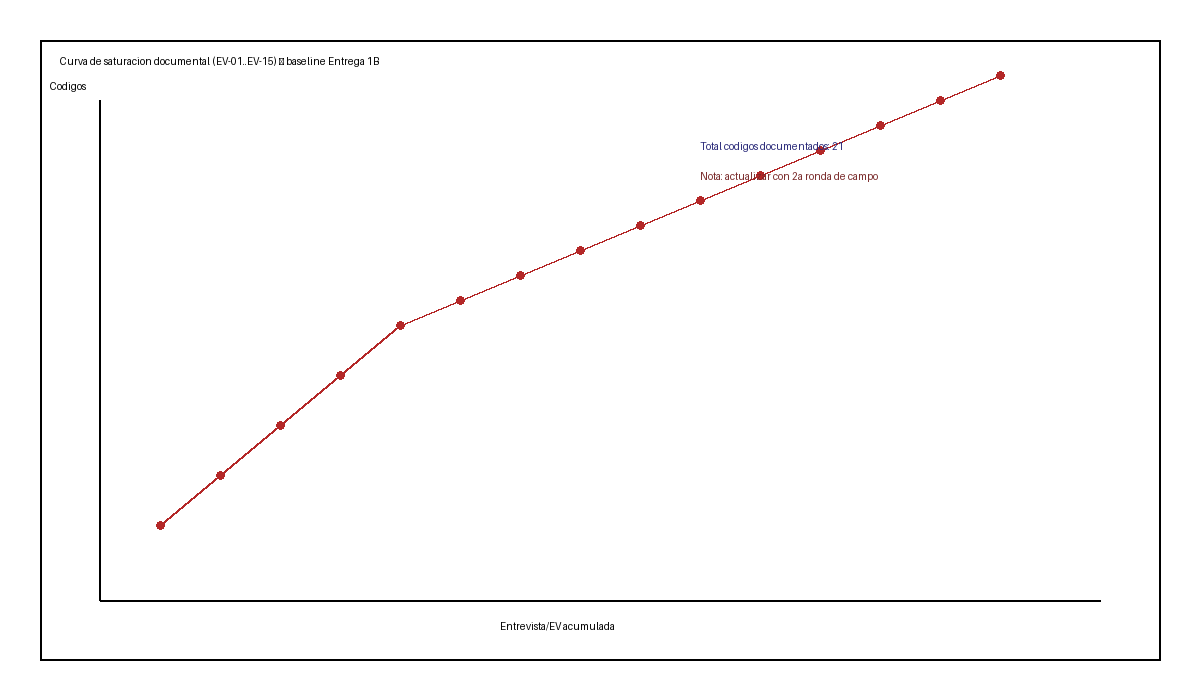
\includegraphics[width=0.88\textwidth]{curva_saturacion.png}\caption{Curva de saturación documental preliminar; actualizar tras la segunda ronda \cite{hennink2017saturation}.}\end{figure}

\section{Componente empírico: protocolo experimental}
\subsection{Selección del enfoque}
\textbf{Enfoque seleccionado:} Enfoque~1 --- comparar la calidad de RF elicitados por el equipo humano frente a RF generados por un LLM a partir del mismo material fuente \cite{cheng2026genai,vogelsang2024llm,montgomery2022quality}.\\
\textbf{Justificación:} el repositorio ya contempla \path{Experimento/Prompts_LLM/} y existe un corpus de hallazgos EV-01--EV-15 más transcripción/entrevista de personal bibliotecario; SIGBUNI además tiene componentes de IA, pero la pregunta empírica priorizada es la calidad de requisitos en elicitación asistida por LLM.\\
\textbf{URL y fecha del registro OSF previo:} \pendiente{registrar en \url{https://osf.io} \emph{antes} de ejecutar el experimento; adjuntar \path{Experimento/osf_registration.pdf}}.

\subsection{Preguntas de investigación mediante PICOC}
\begin{table}[H]\centering
\caption{Marco PICOC del experimento (Enfoque 1)}
\begin{tabularx}{\textwidth}{P{0.18\textwidth}Y}\toprule
Población & Conjuntos de RF sobre SIGBUNI (mínimo 50 RF por conjunto) evaluados por $\geq$3 expertos independientes.\\
Intervención & Generación de RF con LLM (modelo, temperatura, top-$p$ y semilla fijados) a partir de material fuente anonimizado.\\
Comparación & RF elicitados por el equipo humano a partir del mismo material fuente.\\
Resultado (Outcome) & Puntuaciones 1--5 en completitud, ausencia de ambigüedad, verificabilidad, corrección respecto de la fuente y consistencia interna; $\kappa$ interevaluador; tamaño del efecto.\\
Contexto & Biblioteca universitaria UTEQ / proyecto SIGBUNI (ISR401).\\\bottomrule
\end{tabularx}
\end{table}

\begin{enumerate}[label=RQ\arabic*:]
\item ¿En qué dimensiones de calidad difieren los RF humanos de los generados por un LLM a partir del mismo material fuente de SIGBUNI?
\item ¿Cuál es el acuerdo interevaluador ($\kappa$ de Cohen/Fleiss) al puntuar a ciegas ambos conjuntos?
\item ¿Qué amenazas a la validez limitan la generalización del resultado al dominio bibliotecario universitario?
\end{enumerate}

\subsection{Hipótesis o proposiciones}
\textbf{H0-1:} No existe diferencia significativa entre la puntuación media de calidad de RF humanos y RF generados por LLM.\\
\textbf{H1-1:} Existe diferencia significativa en al menos una dimensión de calidad (prueba $t$ apareada o Wilcoxon; $\alpha=0{,}05$).\\
\textbf{H0-2:} El acuerdo interevaluador no supera $\kappa=0{,}40$ (acuerdo pobre/moderado bajo).\\
\textbf{H1-2:} El acuerdo interevaluador alcanza al menos $\kappa\geq0{,}40$ tras calibración de la rúbrica.

\subsection{Variables}
\begin{longtable}{P{0.20\textwidth}P{0.25\textwidth}P{0.30\textwidth}P{0.18\textwidth}}\toprule
\textbf{Tipo} & \textbf{Variable} & \textbf{Operacionalización} & \textbf{Escala}\\\midrule\endfirsthead
\toprule\textbf{Tipo} & \textbf{Variable} & \textbf{Operacionalización} & \textbf{Escala}\\\midrule\endhead
Independiente & Origen del RF & Humano vs LLM & Nominal\\
Dependiente & Calidad del RF & Media de 5 dimensiones de la rúbrica & 1--5 ordinal/intervalo\\
Dependiente & Acuerdo & Cohen $\kappa$ / Fleiss $\kappa$ & $[-1,1]$\\
Control & Material fuente, prompt, modelo, temperatura, top-$p$, semilla, rúbrica & Fijos y versionados & ---\\\bottomrule
\end{longtable}

\subsection{Participantes, muestreo y ética}
\textbf{Población y muestra:} $\geq$3 evaluadores independientes (recomendado 5) del área de ingeniería de software/requisitos; conjuntos A/B con $\geq$50 RF cada uno.\\
\textbf{Potencia:} se fija $\alpha=0{,}05$, potencia $1-\beta=0{,}80$ y tamaño de efecto medio ($d=0{,}5$) según prácticas de \cite{molleri2020surveys,wohlin2012experimentation}; el tamaño final se reportará en el registro OSF.\\
\textbf{Reclutamiento:} estudiantes avanzados u otros docentes del paralelo, sin participación en la redacción del conjunto humano.\\
\textbf{Consentimiento y anonimización:} consentimiento específico del experimento; material fuente sin datos personales identificables.\\
\textbf{LOPDP:} tratamiento con finalidad de investigación y publicación de datos anonimizados \cite{lopdp2021}.

\subsection{Instrumentos y replicabilidad}
\begin{itemize}
\item Guion/material fuente anonimizado: entrevista bibliotecaria + hallazgos EV.
\item Rúbrica experta 1--5 (completitud, no ambigüedad, verificabilidad, corrección, consistencia).
\item Prompt LLM versionado en \path{Experimento/Prompts_LLM/} con modelo, temperatura, top-$p$, top-$k$ y semilla.
\item Plantilla de consentimiento del experimento en \path{Experimento/Instrumentos/}.
\end{itemize}

\subsection{Plan de análisis estadístico}
\begin{enumerate}
\item Limpieza y apareamiento de RF; cegamiento del origen para evaluadores.
\item Shapiro--Wilk sobre diferencias apareadas.
\item Prueba $t$ apareada o Wilcoxon según normalidad.
\item Tamaño del efecto Cohen $d$ o Cliff $\delta$.
\item Cohen $\kappa$ por pares y Fleiss $\kappa$ global \cite{cohen1960kappa,fleiss1971kappa}.
\item Corrección de Bonferroni si se contrastan las cinco dimensiones.
\item Scripts en \path{Experimento/Scripts_Analisis/} que regeneren tablas/figuras.
\end{enumerate}

\subsection{Resultados}
No se redactan resultados numéricos hasta ejecutar el protocolo \emph{después} del registro OSF y generar salidas desde scripts versionados.

\subsection{Amenazas a la validez}
\begin{tabularx}{\textwidth}{P{0.18\textwidth}Y Y}\toprule
\textbf{Categoría} & \textbf{Amenaza} & \textbf{Mitigación y limitación remanente}\\\midrule
Interna & Sesgo de evaluación si se conoce el origen del RF & Cegamiento A/B; calibración previa; limitación: fuga accidental de estilo.\\
Externa & Un solo dominio (biblioteca UTEQ) & Se reporta como estudio de caso contextual; no se generaliza a todo RE.\\
Constructo & La rúbrica puede no capturar toda la calidad & Cinco dimensiones alineadas a \cite{montgomery2022quality}; posible constructo incompleto.\\
Conclusión & Muestra pequeña de evaluadores & Potencia a priori; reportar ICs; limitación si $n<5$.\\\bottomrule
\end{tabularx}

\section{Preparación de publicación y datos FAIR}
\subsection{Paquete de datos}
El paquete para Zenodo debe incluir transcripciones anonimizadas en JSON, respuestas en CSV, corpus RF/RNF etiquetado, matriz de trazabilidad, prompts y respuestas de LLM cuando apliquen, scripts y un \path{README_dataset.md}. Los principios FAIR se documentarán siguiendo \cite{wilkinson2016fair}.

\begin{longtable}{P{0.30\textwidth}P{0.34\textwidth}P{0.28\textwidth}}\toprule
\textbf{Artefacto} & \textbf{Formato/ubicación} & \textbf{Estado}\\\midrule\endfirsthead
\toprule\textbf{Artefacto} & \textbf{Formato/ubicación} & \textbf{Estado}\\\midrule\endhead
Transcripciones anonimizadas & JSON / \path{Publicacion/DataSet_Zenodo/} & Estructura lista; faltan JSON anonimizados\\
Respuestas de cuestionario & CSV & Pendiente exportación desde PDF manuscrito\\
Corpus RF/RNF & JSON & Pendiente export desde este ERS\\
Matriz de trazabilidad & CSV & Disponible en \path{Trazabilidad/matriz_trazabilidad.csv}\\
Prompts y respuestas LLM & Markdown/JSON & Carpeta \path{Experimento/Prompts_LLM/} lista\\
Scripts de análisis & Python & Plantilla en \path{Experimento/Scripts_Analisis/}\\
Diccionario y citación & \path{README_dataset.md} & Borrador en dataset_zenodo\\
Licencia & CC BY 4.0 para datos/documento & Declarada en LICENSE raíz\\
DOI Zenodo & URL/DOI persistente & Pendiente depósito\\\bottomrule
\end{longtable}

\subsection{Borrador de manuscrito paralelo}
\textbf{Título preliminar:} Comparación empírica de la calidad de requisitos elicitados por humanos y por un LLM en un sistema bibliotecario universitario.\\
\textbf{Resumen preliminar (sin resultados):} \emph{Contexto:} la GenAI se usa cada vez más en RE, pero la evidencia empírica en dominios latinoamericanos es limitada \cite{cheng2026genai,arora2024llm}. \emph{Objetivo:} comparar RF humanos y RF de LLM sobre SIGBUNI. \emph{Método:} cuasi-experimento apareado con rúbrica de cinco dimensiones, $\geq$3 evaluadores ciegos y análisis de $\kappa$ y tamaño del efecto. \emph{Resultados/Conclusiones:} se completarán tras el registro OSF y la ejecución.\\
\textbf{Palabras clave:} Ingeniería de Requerimientos; Modelos Grandes de Lenguaje; Calidad de requisitos; Estudio empírico; Biblioteca universitaria.

\subsubsection{Introducción del manuscrito}
SIGBUNI digitaliza préstamos, catálogo, reservas, acceso e IA en la biblioteca UTEQ. La literatura reciente muestra adopción de LLM en RE, pero con vacíos en validación empírica y en contextos latinoamericanos \cite{cheng2026genai,vogelsang2024llm}. Contribuciones previstas: (1) dataset apareado humano--LLM de RF; (2) medición multidimensional de calidad con acuerdo interevaluador; (3) amenazas a la validez explícitas. Las RQ se detallan en la Sección del protocolo.

\subsubsection{Trabajo relacionado}
\textbf{Cadena de búsqueda:} (\texttt{"requirements engineering"} OR \texttt{"software requirements"}) AND (\texttt{"large language model"} OR ChatGPT OR Claude) AND (elicitation OR quality).\\
\textbf{Bases:} Scopus y Google Scholar (últimos tres años).\\
\textbf{Inclusión:} peer-reviewed con datos empíricos en RE; \textbf{exclusión:} editoriales, short papers $<$4 páginas, estudios sin datos.\\
\textbf{Cuadro comparativo:} se construirá con 10--15 trabajos cercanos (p.~ej. \cite{cheng2026genai,montgomery2022quality,ferrari2016ambiguity,fischbach2023acceptance}) tras ejecutar la búsqueda y registrar conteos.

\subsubsection{Metodología}
Idéntica al protocolo Enfoque~1 (PICOC, hipótesis, variables, instrumentos y plan estadístico). Se sigue la plantilla de reporte experimental de \cite{jedlitschka2008reporting,wohlin2012experimentation}.

\subsubsection{Resultados, discusión y conclusiones}
Se completan exclusivamente después de ejecutar el estudio y analizar los datos con scripts versionados.

\subsection{Análisis de revistas objetivo}
Candidatas mixtas (APC y suscripción/híbrida). Indicadores a revalidar en las herramientas oficiales al momento del envío.

\small
\begin{longtable}{P{0.09\textwidth}P{0.22\textwidth}P{0.10\textwidth}P{0.07\textwidth}P{0.10\textwidth}P{0.10\textwidth}P{0.16\textwidth}}\toprule
\textbf{Editorial} & \textbf{Revista} & \textbf{JCR/Q} & \textbf{IF} & \textbf{Modelo} & \textbf{APC} & \textbf{Ajuste}\\\midrule\endfirsthead
\toprule\textbf{Editorial} & \textbf{Revista} & \textbf{JCR/Q} & \textbf{IF} & \textbf{Modelo} & \textbf{APC} & \textbf{Ajuste}\\\midrule\endhead
Springer & Requirements Engineering & Q2 & 3{,}3 & Híbrida & OA opcional & Ajuste alto al tema RE\\
Springer & Empirical Software Engineering & Q1/Q2 & Verificar & Híbrida & OA opcional & Métodos empíricos\\
Elsevier & Inf. and Software Technology & Verificar & Verificar & Híbrida & OA opcional & RE/SE empírico\\
Elsevier & J. Systems and Software & Verificar & Verificar & Híbrida & OA opcional & Calidad software\\
IEEE & IEEE Access & Q2 (típ.) & Verificar & OA (APC) & Sí (APC) & Difusión rápida\\
IEEE & IEEE Trans. Software Eng. & Q1 & Verificar & Híbrida & OA opcional & Alto impacto; mayor exigencia\\\bottomrule
\end{longtable}
\normalsize
Detalle operativo en \path{Publicacion/analisis_revistas.md}.

\subsection{Disponibilidad de datos y materiales}
\textbf{DOI de Zenodo:} pendiente de depósito al envío.\\
\textbf{Registro OSF:} pendiente (obligatorio antes del experimento).\\
\textbf{Licencia del dataset:} CC BY 4.0.\\
\textbf{Citación:} conforme a \cite{smith2016software,druskat2021cff} vía \path{CITATION.cff}.

\section{Estructura y verificación del repositorio}
\subsection{Árbol obligatorio}
\begin{Verbatim}[fontsize=\small]
SIGBUNI_ISR401/
  README.md
  LICENSE
  CITATION.cff
  CHANGELOG.md
  .gitignore
  checksums.sha256
  01_ERS/
    ERS_SRS_2A_v1.0.pdf
    ERS_SRS_2A_v1.0.tex
    referencias.bib
  02_Evidencias/
    Consentimientos/ Video/ Audio/ Fotos_Entorno/
    Cuestionario/Fotos_Aplicacion/ Cuestionario/Respuestas/
    Documentos_Organizacion/ Validacion_Walkthrough/
    Codificacion_Tematica/
  03_Modelado/Diagramas_UML/  03_Modelado/Mockups/
  04_Trazabilidad/
    matriz_trazabilidad.csv
    priorizacion_moscow_kano.csv
  05_MVP/README.md  05_MVP/video_demo.mp4
  06_Experimento/
    protocolo.pdf  osf_registration.pdf  instrumentos/
    prompts_llm/ resultados/ scripts_analisis/
  07_Publicacion/
    manuscrito_borrador.pdf  dataset_zenodo/
\end{Verbatim}

\subsection{Archivos raíz obligatorios}
\begin{tabularx}{\textwidth}{P{0.22\textwidth}Y P{0.14\textwidth}}\toprule
\textbf{Archivo} & \textbf{Contenido mínimo} & \textbf{Estado}\\\midrule
README.md & Sistema, integrantes/roles, enlaces, reproducción y TOC. & Actualizado\\
LICENSE & MIT (código MVP) + CC BY 4.0 (datos/documento). & Actualizado\\
CITATION.cff & Autores, título, versión y fecha (ORCID/DOI pendientes). & Actualizado\\
CHANGELOG.md & Historial desde 1A hasta 1.1. & Actualizado\\
checksums.sha256 & Hashes de multimedia verificable. & Actualizado\\\bottomrule
\end{tabularx}

\subsection{Checklist de aceptación y gatekeepers}
\begin{longtable}{P{0.06\textwidth}P{0.78\textwidth}P{0.10\textwidth}}\toprule
\textbf{ID} & \textbf{Comprobación} & \textbf{Estado}\\\midrule\endfirsthead
\toprule\textbf{ID} & \textbf{Comprobación} & \textbf{Estado}\\\midrule\endhead
CK-01 & Estructura de carpetas alineada (ERS/Evidencias/Modelado/...). & Parcial (falta renombrar a 01\_--07\_)\\
CK-02 & Cinco archivos raíz completos. & Cumple\\
CK-03 & PDF unificado desde LaTeX, historial y enlace GitHub. & Fuente lista; compilar PDF\\
CK-04 & Nomenclatura estándar de multimedia. & Parcial\\
CK-05 & Audio válido con ffprobe ($>$0\,s). & 1 audio OK; videos faltan\\
CK-06 & Consentimientos legibles y firmados. & 10 OK\\
CK-07 & Cuestionario con fotos y $n\geq30$. & PDF presente; falta CSV/fotos\\
CK-08 & Protocolo OSF registrado antes de ejecutar. & Pendiente\\
CK-09 & Prompts con parámetros reproducibles. & Plantilla lista\\
CK-10 & Scripts reproducen tablas y figuras. & Plantilla lista\\
CK-11 & Hashes SHA-256 coinciden. & Generado\\
CK-12 & Matriz $\geq$40 filas y columnas obligatorias. & 45 filas OK\\
CK-13 & Toda evidencia declarada existe y es verificable. & Parcial (inventario honesto)\\
CK-14 & 25 RF, 15 RNF, $\geq$10 CU y explicabilidad IA. & Cumple\\
CK-15 & MVP ejecutable con $\geq$60\% RF Must. & No cumple aún\\\bottomrule
\end{longtable}

\section{Conclusiones y trabajo pendiente}
Este ERS/SRS consolida SIGBUNI para la Entrega 3 (2A) con \textbf{25 RF}, \textbf{15 RNF} (incluidas explicabilidades de IA), mapeo LOPDP, historias Connextra/Gherkin para RF Must, \textbf{13 CU} detallados, UML (secuencia, actividad, estados, componentes, despliegue e i*), priorización MoSCoW+Kano+WSJF, matriz de trazabilidad con \textbf{45 filas}, mockups Visily trazados y protocolo empírico Enfoque~1.

\textbf{Pendiente crítico para gatekeepers/C7--C10:} videos de la segunda ronda, audios adicionales, fotos fechadas, walkthroughs con acta, exportación CSV del cuestionario ($n\geq30$), registro OSF previo, MVP ejecutable con $\geq$60\% RF Must, video demo y depósito FAIR/Zenodo. No se fabrican resultados experimentales ni evidencias multimedia ausentes del repositorio.

\section{Cierre terminal de la Entrega 4 (2B)}
\label{sec:cierre2b}

La Entrega 4 (2B) constituye el cierre del Proyecto Fin de Curso de SIGBUNI. 
En esta versión se consolida la ERS/SRS v2.0, se cierra el componente empírico,
se prepara el paquete de replicación FAIR y se documentan los materiales de
publicación y defensa. Todo resultado cuantitativo o cualitativo reportado en
esta sección debe ser reproducible a partir de los datos y scripts versionados
en el repositorio; no se incorporan cifras hipotéticas ni evidencias no
verificadas.

\subsection{Estado de la línea base de la ERS/SRS v2.0}

La línea base terminal debe publicarse como \texttt{ERS\_SRS\_2B\_v2.0.tex} y
\texttt{ERS\_SRS\_2B\_v2.0.pdf}. La versión 2.0 debe integrar las correcciones
docentes acumuladas, eliminar secciones pendientes que ya cuenten con evidencia,
mantener un único documento coherente y enlazar los artefactos de modelado,
trazabilidad, MVP y evidencia empírica.

\begin{table}[H]
\centering
\caption{Control terminal de la ERS/SRS para la Entrega 4 (2B)}
\begin{tabularx}{\textwidth}{P{0.28\textwidth}Y P{0.18\textwidth}}
\toprule
\textbf{Elemento} & \textbf{Criterio terminal} & \textbf{Estado} \\
\midrule
Versión documental & ERS/SRS unificada y versionada como v2.0 & \pendiente{verificar versión final} \\
Observaciones docentes & Todas las observaciones de 2A resueltas & \pendiente{cerrar observaciones} \\
Trazabilidad & Al menos 60 filas cerradas y consistentes & \pendiente{ampliar y validar matriz} \\
UML & Diagramas consistentes con el MVP final & \pendiente{verificar contra código} \\
MVP & Cobertura mínima del 80\% de RF Must have & \pendiente{medir cobertura real} \\
\bottomrule
\end{tabularx}
\end{table}

\subsection{Trazabilidad terminal}
\label{subsec:trazabilidad_terminal}

La matriz terminal debe conectar, como mínimo, la fuente o evidencia,
objetivo, stakeholder, requisito, caso de uso, criterio de aceptación,
componente, modelo, mockup o interfaz y evidencia de prueba. Para esta entrega,
la matriz debe contener al menos 60 filas cerradas. Las filas nuevas deben
corresponder a trazas reales; no se añaden enlaces únicamente para alcanzar
el mínimo numérico.

La matriz vigente de la Entrega 3 contiene 45 filas documentadas. Por tanto,
antes del cierre se requiere revisar los artefactos actuales y añadir las
trazas faltantes que realmente existan, especialmente las asociadas al MVP,
pruebas, componentes de IA, datos y escenarios de demostración. Las nuevas
filas deben conservar identificadores únicos y permitir trazabilidad
bidireccional.

\subsection{Cobertura terminal del MVP}
\label{subsec:mvp_terminal}

La cobertura del MVP se recalcula sobre el conjunto definitivo de RF
clasificados como \emph{Must have}. Si se mantiene la línea base actual de
16 RF Must, el umbral del 80\% exige al menos 13 RF Must implementados y
demostrables. El valor final debe calcularse con la fórmula:

\[
\text{Cobertura MVP} =
\frac{\#\text{RF Must implementados y verificables}}
{\#\text{RF Must totales}}
\times 100.
\]

\noindent
\textbf{Cobertura final verificada:}
\pendiente{insertar numerador, denominador, porcentaje y evidencia del MVP real}.

La demostración debe utilizar un entorno estable y cubrir dos escenarios
seleccionados previamente desde la matriz de trazabilidad. Las credenciales
utilizadas durante la defensa deben ser exclusivamente credenciales de
demostración.

\section{Trabajo de campo terminal, evidencia y privacidad}
\label{sec:campo_terminal}

\subsection{Mínimos empíricos de cierre}

La Entrega 4 eleva los mínimos de evidencia respecto de la Entrega 3. El
inventario final debe verificarse contra los archivos reales del repositorio,
sus metadatos y, cuando corresponda, sus hashes SHA-256.

\begin{longtable}{P{0.28\textwidth}P{0.25\textwidth}P{0.37\textwidth}}
\toprule
\textbf{Evidencia} & \textbf{Mínimo terminal} & \textbf{Ubicación esperada} \\
\midrule
\endfirsthead
\toprule
\textbf{Evidencia} & \textbf{Mínimo terminal} & \textbf{Ubicación esperada} \\
\midrule
\endhead
Consentimientos & $\geq 16$ participantes distintos acumulados; 24 recomendado & \path{02_Evidencias/Consentimientos/} (copia pública enmascarada) y original en zona restringida \\
Videos de entrevistas & $\geq 16$ archivos y duración total $\geq 240$ minutos & Contenedor cifrado de \path{02_Evidencias/00_Restringido/} + ficha técnica pública \\
Audios de entrevistas & $\geq 16$ archivos, redundantes con los videos & Contenedor cifrado + ficha técnica pública \\
Transcripciones & Una transcripción anonimizada por entrevista & \path{02_Evidencias/Transcripciones/} \\
Cuestionario & $n \geq 60$ por perfil dominante o cálculo de potencia explícito & \path{02_Evidencias/Cuestionario/Respuestas/} \\
Documentos organización & $\geq 5$ documentos de tipos distintos & \path{02_Evidencias/Documentos_Organizacion/} \\
Walkthrough & $\geq 6$ sesiones: 3 técnicas + 3 no técnicas & \path{02_Evidencias/Validacion_Walkthrough/} \\
Member checking & 1 sesión con $\geq 3$ participantes previos & \path{02_Evidencias/Member_Checking/} \\
Codificación temática & Tabla cerrada + curva de saturación, cuando aplique & \path{02_Evidencias/Codificacion_Tematica/} \\
\bottomrule
\end{longtable}

\subsection{Zonas pública y restringida}

La evidencia se divide en dos zonas. La zona pública [P] contiene únicamente
material anonimizado o enmascarado. La zona restringida [R] contiene material
identificable y debe almacenarse cifrada con AES-256 en
\path{02_Evidencias/00_Restringido/}. La contraseña no se guarda en GitHub.

Los consentimientos originales, grabaciones sin anonimizar, firmas, cédulas,
rostros, voces y otros identificadores directos pertenecen exclusivamente a la
zona restringida. En la zona pública se utilizan códigos de participante y
copias enmascaradas. El archivo \texttt{fichas\_tecnicas.csv} debe permitir
contrastar los archivos audiovisuales y \texttt{checksums.sha256} debe
contener los hashes verificables.

\subsection{Sesión de miembro-verificación}

Al cierre del análisis se realizará una sesión de \emph{member checking} con
al menos tres participantes que hayan formado parte del estudio. El objetivo
es contrastar la interpretación de los hallazgos con quienes aportaron
información al estudio. El acta pública debe estar enmascarada y la grabación,
si existe, debe permanecer en la zona restringida.

\textbf{Fecha y participantes codificados:}
\pendiente{registrar únicamente después de ejecutar la sesión}.

\section{Componente empírico final: Enfoque 1, humano frente a LLM}
\label{sec:experimento_final}

\subsection{Pregunta de investigación principal}

Para SIGBUNI se mantiene el Enfoque 1 (LLM frente a humano), alineado con el
dominio de biblioteca universitaria. La pregunta principal se formula como:

\begin{quote}
\textbf{RQ1.} ¿En qué medida un LLM puede replicar la elicitación de requisitos
funcionales de un sistema bibliotecario a partir de documentos y transcripciones
anonimizadas, comparado con analistas humanos?
\end{quote}

Como pregunta complementaria se conserva la evaluación de las dimensiones de
calidad de los RF:

\begin{quote}
\textbf{RQ2.} ¿En qué dimensiones de calidad difieren los RF elicitados por
analistas humanos y los RF generados por un LLM a partir del mismo material
fuente anonimizado?
\end{quote}

Las dimensiones de evaluación son completitud, ausencia de ambigüedad,
verificabilidad, corrección respecto de la fuente y consistencia interna.

\subsection{Diseño y variables}

El estudio utiliza un diseño apareado: el conjunto humano y el conjunto LLM se
construyen a partir del mismo material fuente anonimizado. Los evaluadores
califican los requisitos sin conocer el origen de cada conjunto cuando el
procedimiento de cegamiento sea viable.

\begin{longtable}{P{0.21\textwidth}P{0.26\textwidth}P{0.43\textwidth}}
\toprule
\textbf{Tipo} & \textbf{Variable} & \textbf{Operacionalización} \\
\midrule
\endfirsthead
\toprule
\textbf{Tipo} & \textbf{Variable} & \textbf{Operacionalización} \\
\midrule
\endhead
Independiente & Origen del requisito & Humano / LLM \\
Dependiente & Calidad del requisito & Puntuación por las cinco dimensiones definidas \\
Dependiente & Acuerdo entre evaluadores & $\kappa$ de Cohen por pares y $\kappa$ de Fleiss para tres o más evaluadores \\
Control & Material fuente & Mismo corpus anonimizado para ambos conjuntos \\
Control & Configuración del LLM & Modelo, versión, temperatura, top-$p$, semilla y fecha/hora documentados \\
Control & Instrumento de evaluación & Misma rúbrica y procedimiento para ambos conjuntos \\
\bottomrule
\end{longtable}

\subsection{Plan de análisis estadístico reproducible}

Todo el análisis debe ejecutarse mediante scripts versionados en
\path{06_Experimento/scripts_analisis/}. El procedimiento terminal incluye:

\begin{enumerate}
    \item Importación y validación de los datos crudos.
    \item Limpieza documentada y generación de los datos procesados.
    \item Estadísticos descriptivos por grupo y dimensión: media, mediana,
          desviación estándar, mínimo, máximo e intervalo intercuartílico.
    \item Prueba de Shapiro--Wilk para evaluar normalidad de las diferencias
          apareadas.
    \item Prueba de Levene cuando corresponda comprobar homogeneidad de
          varianzas.
    \item Comparación apareada mediante prueba $t$ para muestras apareadas si
          se satisfacen los supuestos; en caso contrario, prueba de Wilcoxon
          de rangos con signo.
    \item Corrección de Holm--Bonferroni cuando se realicen múltiples
          comparaciones entre dimensiones.
    \item Tamaño del efecto mediante $d$ de Cohen para el análisis paramétrico
          o $\delta$ de Cliff para el análisis no paramétrico.
    \item Intervalos de confianza del 95\% mediante \emph{bootstrap} de
          10\,000 réplicas para los tamaños del efecto cuando aplique.
    \item Acuerdo interevaluador mediante $\kappa$ de Cohen por pares y
          $\kappa$ de Fleiss cuando participen tres o más evaluadores.
    \item Generación automática de todas las tablas y figuras utilizadas en
          el manuscrito.
\end{enumerate}

Cada prueba reportada debe incluir el nombre exacto, el estadístico calculado,
el valor $p$ con al menos tres decimales, el tamaño del efecto y su intervalo
de confianza del 95\%. Las desviaciones respecto del protocolo registrado
previamente deben declararse tanto en el manuscrito como en
\texttt{osf\_deviations.pdf}.

\subsection{Resultados por pregunta de investigación}

Esta subsección se completa exclusivamente después de ejecutar los scripts
sobre los datos reales.

\subsubsection{Resultados de RQ1}
\pendiente{insertar tablas, figuras y estadísticos generados por scripts; no escribir resultados hipotéticos}.

\subsubsection{Resultados de RQ2}
\pendiente{insertar tablas, figuras y estadísticos generados por scripts; no escribir resultados hipotéticos}.

\section{Discusión}
\label{sec:discusion2b}

La discusión final se organiza en tres bloques: implicaciones para la
investigación, implicaciones para la práctica y hallazgos sorprendentes o
contraintuitivos. Cada afirmación debe rastrearse a un resultado reproducible o
a una referencia bibliográfica. Las conclusiones se restringen al dominio,
muestra y diseño de SIGBUNI y no se generalizan a todos los proyectos de
ingeniería de requisitos.

\subsection{Implicaciones para la investigación}
\pendiente{redactar a partir de RQ1/RQ2 y referencias verificadas}.

\subsection{Implicaciones para la práctica}
\pendiente{redactar a partir de hallazgos observados en SIGBUNI}.

\subsection{Hallazgos sorprendentes o contraintuitivos}
\pendiente{incluir únicamente si aparecen en los resultados reales}.

\section{Amenazas a la validez}
\label{sec:amenazas2b}

Las amenazas se organizan en las cuatro categorías exigidas para estudios
empíricos en ingeniería de software. Se documentan al menos dos amenazas por
categoría y la mitigación aplicada.

\begin{longtable}{P{0.16\textwidth}P{0.33\textwidth}P{0.41\textwidth}}
\toprule
\textbf{Validez} & \textbf{Amenaza} & \textbf{Mitigación y limitación remanente} \\
\midrule
\endfirsthead
\toprule
\textbf{Validez} & \textbf{Amenaza} & \textbf{Mitigación y limitación remanente} \\
\midrule
\endhead
Interna & Los evaluadores podrían inferir si un RF fue escrito por humanos o por un LLM a partir del estilo. & Usar identificadores neutrales, mezclar el orden y aplicar cegamiento cuando sea viable; el estilo puede seguir actuando como pista residual. \\
Interna & Diferencias en el material fuente o en el preprocesamiento podrían favorecer a un grupo. & Usar el mismo corpus anonimizado y documentar cualquier transformación; persiste el riesgo de pérdidas durante la anonimización. \\
Externa & El estudio se realiza en un único sistema bibliotecario universitario ecuatoriano. & Delimitar explícitamente el alcance y publicar el paquete de replicación para facilitar estudios en otros dominios. \\
Externa & La composición de participantes y evaluadores puede no representar a todas las universidades. & Describir perfiles, criterios de inclusión y contexto; evitar generalizaciones poblacionales no sustentadas. \\
Constructo & Una rúbrica de cinco dimensiones puede no capturar toda la calidad de un requisito. & Justificar las dimensiones con literatura de calidad de requisitos y reportar el instrumento completo. \\
Constructo & La puntuación de calidad depende del juicio humano de los evaluadores. & Calibrar la rúbrica y cuantificar el acuerdo con $\kappa$ de Cohen/Fleiss. \\
Conclusión & Un tamaño muestral insuficiente puede reducir la potencia estadística. & Ejecutar el cálculo de potencia o justificar el tamaño muestral, reportar intervalos de confianza y tamaños del efecto. \\
Conclusión & Comparaciones múltiples aumentan el riesgo de falsos positivos. & Aplicar Holm--Bonferroni y declarar todas las comparaciones planificadas previamente. \\
\bottomrule
\end{longtable}

\section{Manuscrito final y estrategia de publicación}
\label{sec:publicacion2b}

\subsection{Revista o conferencia objetivo}

Antes de cerrar el manuscrito, el equipo debe mantener una única revista o
conferencia primaria previamente declarada al docente. El manuscrito final debe
usar exclusivamente la plantilla oficial de esa sede. Si la revista objetivo
es \emph{Requirements Engineering} de Springer Nature, debe migrarse a la
plantilla oficial correspondiente; el formato IEEEtran utilizado en la ERS no
sustituye la plantilla editorial del manuscrito.

\subsection{Estructura obligatoria del manuscrito}

El manuscrito final separado debe contener:

\begin{enumerate}
    \item Título específico de 10 a 15 palabras.
    \item Autoría, filiación, correos institucionales y ORCID.
    \item Resumen estructurado de 200 a 250 palabras:
          Contexto--Objetivo--Método--Resultados--Conclusiones.
    \item Entre tres y cinco palabras clave.
    \item Introducción.
    \item Trabajo relacionado con búsqueda sistemática cerrada y comparación
          de 10 a 15 estudios cercanos.
    \item Metodología replicable con PICOC, hipótesis, variables, diseño,
          participantes, instrumentos, análisis y desviaciones del protocolo.
    \item Resultados organizados por RQ.
    \item Discusión.
    \item Amenazas a la validez.
    \item Conclusiones y trabajo futuro.
    \item \emph{Data and materials availability}.
    \item Declaración de tecnologías de IA asistida y agradecimientos.
    \item Referencias verificadas según el estilo de la revista o conferencia.
\end{enumerate}

El archivo se versiona en \path{07_Publicacion/manuscrito_final.tex} y su PDF
en \path{07_Publicacion/manuscrito_final.pdf}. Los datos, tablas y figuras del
manuscrito deben poder regenerarse mediante los scripts de análisis.

\subsection{Trabajo relacionado y referencias}

La revisión abreviada se cierra con 10 a 15 trabajos directamente relacionados.
El cuadro comparativo debe incluir referencia, año, tipo de estudio, población,
intervención, resultados principales y diferencia con SIGBUNI.

La bibliografía final debe contener al menos 40 entradas verificadas. Cada DOI
debe resolver a la publicación citada cuando exista. Las entradas marcadas
como provisionales o con metadatos por verificar deben corregirse o retirarse
antes del cierre.

\section{Disponibilidad de datos, FAIR y ciencia abierta}
\label{sec:fair2b}

\subsection{Zenodo}

El paquete de replicación se construye desde
\path{07_Publicacion/dataset_zenodo/} y se deposita en Zenodo. El DOI final se
incorpora al README, al archivo \texttt{CITATION.cff} y a la sección de
disponibilidad de datos del manuscrito.

\textbf{DOI de Zenodo:}
\pendiente{insertar DOI real después del depósito}.

\subsection{OSF}

El registro OSF debe conservar el protocolo pre-registrado y documentar
explícitamente las desviaciones mediante
\path{06_Experimento/osf_deviations.pdf}.

\textbf{Registro OSF:}
\pendiente{insertar URL real del registro}.

\subsection{Software Heritage}

El repositorio final debe archivarse en Software Heritage mediante
\emph{Save code now}. El SWHID resultante se incorpora en el README y en
\texttt{CITATION.cff}.

\textbf{SWHID:}
\pendiente{insertar identificador real después del archivado}.

\subsection{Autoevaluación FAIR}

Antes del corte final se ejecuta una autoevaluación FAIR mediante F-UJI o el
modelo FAIR Data Maturity. El reporte se guarda como
\texttt{fair\_assessment.pdf} en la raíz del repositorio. El objetivo de
aceptación es un puntaje agregado igual o superior al 60\%.

\textbf{Puntaje FAIR:}
\pendiente{insertar puntaje real y herramienta utilizada}.

\subsection{Contenido mínimo del paquete de replicación}

El paquete abierto debe contener, como corresponda al estudio, transcripciones
anonimizadas, respuestas de cuestionario sin identificadores directos, corpus
RF/RNF etiquetado, matriz de trazabilidad en CSV, prompts y respuestas del LLM
con parámetros de ejecución, scripts reproducibles,
\texttt{README\_dataset.md}, \texttt{ANONYMIZATION.md} y \texttt{ETHICS.md}.

\section{Ética, anonimización y uso de IA}
\label{sec:etica_ia_2b}

\subsection{Documentación ética}

La documentación ética vigente se concentra en \path{08_Etica/}. Debe incluir
el paquete base A.1--A.13, la documentación específica de la categoría de
riesgo aplicable, el aval institucional, la adenda de segunda ronda y un
README de la carpeta. La documentación identificable no debe exponerse en la
zona pública del repositorio.

\subsection{Declaración de tecnologías de IA asistida}

El uso de herramientas de IA en la preparación del manuscrito debe declararse
de forma transparente. La declaración final debe indicar modelo, versión,
parámetros relevantes cuando se conozcan y uso concreto. La IA puede utilizarse
para apoyo de redacción o revisión sobre contenido producido y verificado por
el equipo; no se utiliza para inventar resultados, cifras, tablas, evidencias
ni conclusiones empíricas.

\begin{quote}
\textbf{Declaración a completar:}
\pendiente{indicar herramienta/modelo, versión, uso concreto y método de validación humana}.
\end{quote}

\section{Estructura obligatoria del repositorio para 2B}
\label{sec:repo2b}

El repositorio terminal debe reorganizarse para coincidir con el siguiente
árbol:

\begin{Verbatim}[fontsize=\small]
SIGBUNI_ISR401/
  README.md
  LICENSE
  CITATION.cff
  CHANGELOG.md
  .gitignore
  checksums.sha256
  fair_assessment.pdf
  01_ERS/
    ERS_SRS_2B_v2.0.pdf
    ERS_SRS_2B_v2.0.tex
    referencias.bib
  02_Evidencias/
    00_Restringido/
      evidencias_restringidas.7z
    fichas_tecnicas.csv
    Consentimientos/
    Transcripciones/
    Fotos_Entorno/
    Cuestionario/
      Fotos_Aplicacion/
      Respuestas/
    Documentos_Organizacion/
    Validacion_Walkthrough/
    Member_Checking/
    Codificacion_Tematica/
  03_Modelado/
  04_Trazabilidad/
  05_MVP/
  06_Experimento/
    protocolo.pdf
    osf_registration.pdf
    osf_deviations.pdf
    instrumentos/
    prompts_llm/
    datos_crudos/
    datos_procesados/
    resultados/
    scripts_analisis/
  07_Publicacion/
    manuscrito_final.pdf
    manuscrito_final.tex
    referencias.bib
    figuras/
    tablas/
    dataset_zenodo/
      ANONYMIZATION.md
      ETHICS.md
      README_dataset.md
  08_Etica/
    A01_Protocolo_Investigacion.pdf
    ...
    A13_...
    Categoria_A/
    Categoria_B/
    Categoria_C/
    Aval_Institucional.pdf
    Adenda_Segunda_Ronda.pdf
    README_Etica.md
  09_Defensa/
    presentacion.pdf
    presentacion.pptx
    guion.pdf
    video_defensa.mp4
    folleto_una_hoja.pdf
\end{Verbatim}

\subsection{Archivos raíz}

El README debe identificar el sistema, integrantes, roles y ORCID; enlazar la
ERS/SRS v2.0, el manuscrito final, Zenodo, OSF y Software Heritage; incluir la
cita recomendada y las instrucciones para reproducir el análisis. El archivo
\texttt{CITATION.cff} debe declarar la versión 2.0, autoría, ORCID, fecha de
liberación, DOI de Zenodo y SWHID. \texttt{CHANGELOG.md} debe cubrir la
evolución desde 1A hasta 2B.

\section{Defensa final}
\label{sec:defensa2b}

La defensa dispone de 25 minutos de presentación y 10 minutos de preguntas.
Todos los integrantes participan con al menos cuatro minutos de intervención.
La secuencia recomendada es:

\begin{enumerate}
    \item Problema y contribuciones: 3 minutos.
    \item Sistema y stakeholders: 3 minutos.
    \item Metodología empírica: 4 minutos.
    \item Resultados: 6 minutos.
    \item Discusión y amenazas a la validez: 4 minutos.
    \item Conclusiones y trabajo futuro: 3 minutos.
    \item Demostración corta del prototipo: 2 minutos.
\end{enumerate}

En \path{09_Defensa/} se depositan la presentación PDF, el editable cuando se
disponga, el guion con tiempos, el video de la defensa y el folleto de una
hoja. La demostración debe cubrir dos escenarios trazados y no utilizar
credenciales reales.

\section{Checklist terminal de SIGBUNI}
\label{sec:checklist2b}

\begin{longtable}{P{0.08\textwidth}P{0.72\textwidth}P{0.13\textwidth}}
\toprule
\textbf{ID} & \textbf{Comprobación} & \textbf{Estado} \\
\midrule
\endfirsthead
\toprule
\textbf{ID} & \textbf{Comprobación} & \textbf{Estado} \\
\midrule
\endhead
2B-01 & ERS/SRS v2.0 unificada y sin fragmentos pendientes de entregas anteriores. & \pendiente{verificar} \\
2B-02 & Matriz de trazabilidad con al menos 60 filas cerradas. & \pendiente{verificar} \\
2B-03 & UML final consistente con el MVP. & \pendiente{verificar} \\
2B-04 & MVP cubre al menos 80\% de los RF Must have. & \pendiente{verificar} \\
2B-05 & Mínimos terminales de entrevistas, audio, video, cuestionario y validación cumplidos. & \pendiente{verificar} \\
2B-06 & Zona restringida AES-256, fichas técnicas y checksums verificados. & \pendiente{verificar} \\
2B-07 & Scripts reproducen todas las tablas y figuras del manuscrito. & \pendiente{verificar} \\
2B-08 & Curva de saturación o cálculo de potencia documentado. & \pendiente{verificar} \\
2B-09 & Manuscrito final en plantilla oficial y con resultados reales. & \pendiente{verificar} \\
2B-10 & Bibliografía con al menos 40 entradas verificadas y DOI válido cuando exista. & \pendiente{verificar} \\
2B-11 & Zenodo con DOI, OSF actualizado, SWHID y FAIR $\geq 60\%$. & \pendiente{verificar} \\
2B-12 & Documentación ética A.1--A.13, aval y adenda vigente en \path{08_Etica/}. & \pendiente{verificar} \\
2B-13 & Materiales completos de defensa en \path{09_Defensa/}. & \pendiente{verificar} \\
2B-14 & No existen datos identificables en la zona pública. & \pendiente{verificar antes de publicar} \\
\bottomrule
\end{longtable}

\section{Conclusiones y trabajo futuro de la Entrega 4 (2B)}
\label{sec:conclusiones2b}

Las conclusiones finales se redactan una vez concluido el análisis y deben
responder explícitamente a las preguntas de investigación, recuperar las
contribuciones prometidas en la introducción y delimitar el alcance de los
hallazgos. El trabajo futuro debe incluir al menos tres líneas concretas que
puedan retomarse utilizando el paquete de datos publicado.

\pendiente{redactar conclusiones únicamente con base en los resultados finales reproducibles}.

\appendices
\section{Catálogo inicial de evidencias}
\begin{longtable}{P{0.12\textwidth}P{0.23\textwidth}P{0.45\textwidth}P{0.13\textwidth}}\toprule
\textbf{EV} & \textbf{Técnica/fuente} & \textbf{Hallazgo documentado} & \textbf{Estado}\\\midrule\endfirsthead
\toprule\textbf{EV} & \textbf{Técnica/fuente} & \textbf{Hallazgo documentado} & \textbf{Estado}\\\midrule\endhead
EV-01 & Entrevista & Préstamo manual, devoluciones y vencimientos con seguimiento reactivo. & Verificar archivo.\\
EV-02 & Encuesta & Necesidad de catálogo actualizado, filtros y estado del material. & Verificar archivo.\\
EV-03 & Observación & Reserva informal, alta demanda e inasistencia. & Verificar archivo.\\
EV-04 & Entrevista & Control manual de ingreso y falta de salida digital. & Verificar archivo.\\
EV-05 & Encuesta & Ayuda digital y orientación personalizada. & Verificar archivo.\\
EV-06 & Análisis de problemática & Dificultad para valorar documentos extensos. & Verificar respaldo.\\
EV-07 & Entrevista & Necesidad de reportes de uso. & Verificar archivo.\\
EV-08 & Encuesta & Preferencia por alertas internas. & Verificar archivo.\\
EV-09 & Observación & Necesidad de gestión de usuarios y roles. & Verificar archivo.\\
EV-10 & Encuesta & Preferencia por préstamo digital o mixto. & Verificar archivo.\\
EV-11 & Entrevista & Necesidad de comunicados masivos. & Verificar archivo.\\
EV-12 & Análisis de problemática & Recomendaciones por historial y carrera. & Verificar respaldo.\\
EV-13 & Acta de encuesta & Importancia del acceso desde casa. & Verificar archivo.\\
EV-14 & Acta de entrevista & Control de aforo en horarios críticos. & Verificar archivo.\\
EV-15 & Evidencia fotográfica & Trabajo de campo en entorno bibliotecario. & Incluida como imagen histórica.\\\bottomrule
\end{longtable}



\nocite{*}
\bibliographystyle{IEEEtran}
\bibliography{referencias}
\end{document}
